\documentclass{dcthesis}

\usepackage[export]{adjustbox} % in preambl
\usepackage[normalem]{ulem}
\usepackage{circuitikz}
\usepackage{subcaption}
\usepackage{graphicx}
\usepackage{setspace}
\usepackage{amssymb,amsthm,amsmath,amstext}
\usepackage{mathrsfs}  % allows nice script font for sheaves
% \usepackage{bm}        % allows bold italic letters in math mode
% \usepackage{mathtools} % allows more extendible arrows
\usepackage{stmaryrd}  % additional nice fonts
\usepackage{mathtools}
\usepackage{geometry}
\usepackage{xy}
\usepackage{algorithm}
\usepackage{algpseudocode}
\usepackage{lipsum}
\usepackage{caption}
\usepackage{circuitikz}
\usepackage{tikz-cd}
\usepackage{bbm}
\usepackage{hyperref}
\usepackage{enumerate}% http://ctan.org/pkg/enumerate
\usepackage{tikz}
\usepackage{tikz-cd}
\usepackage{dirtytalk}
\usetikzlibrary{calc}
\usetikzlibrary{positioning, shapes, shapes.geometric, fit}
\hypersetup{
  colorlinks=true,
  linkcolor=blue,
  filecolor=magenta,
  urlcolor=cyan,
  pdftitle={Overleaf Example},
  pdfpagemode=FullScreen,
}

\makeatletter
\renewcommand{\@chapapp}{}% Not necessary...
\newenvironment{chapquote}[2][2em]
{\setlength{\@tempdima}{#1}%
  \def\chapquote@author{#2}%
  \parshape 1 \@tempdima \dimexpr\textwidth-2\@tempdima\relax%
\itshape}
{\par\normalfont\hfill--\ \chapquote@author\hspace*{\@tempdima}\par\bigskip}
\makeatother

\DeclareCaptionFormat{algor}{%
  \hrulefill\par\offinterlineskip\vskip1pt%
\textbf{#1#2}#3\offinterlineskip\hrulefill}
\DeclareCaptionStyle{algori}{singlelinecheck=off,format=algor,labelsep=space}
\captionsetup[algorithm]{style=algori}

%This version of the thesis template has been updated for the
% February 2017 thesis guidelines provided by the School of Graduate
% and Advanced Studies by David Freund and Daryl DeFord.

%  Some good options are draft and singlespacing, for drafts, and *final*,
%for the final cut, and noheadings, for a printout without headings.
%You can also use the copyright option to add a copyright.  Note:
%final will enforce a bunch of different options, like oneside, 12pt
%and doublespacing, as well as make the margins correct.   Draft, has
%larger margins and is appropriate for twosided printing.

%%%%%%%%%%%%%%%%%%%%%%%%%%%
%%%%    IMPORTANT     %%%%%
%%%%%%%%%%%%%%%%%%%%%%%%%%%
%
%  Because dvips doesn't know/care about the page size of the dvi file
%  its working on, and because its so important that the margins of
%  your thesis are correct you have to make sure that you are using
%  the command dvi -t letter *thesisnamehere*
%
%  If you are using a terminal this is straightforward, but if you are
%  using a tex editing program it make take a little bit of searching
%  before you figure out how to make this work.
%
%  Alternatively, you might consider compiling using pdflatex, which
%  compiles straight to a PDF and doesn't have this problem.

%%%%%%%%%%%%%%%%%%%%%%%%%%%%%%%%%%%%%%%%%%%%%%%%%%
% Additional Packages (add as desired)
%%%%%%%%%%%%%%%%%%%%%%%%%%%%%%%%%%%%%%%%%%%%%%%%%%
\usepackage{amsmath,amssymb,amsthm}

%\usepackage{mkindex} %Uncomment if you would like to have an index.
% Compiling with an index takes more work than compiling without one.
% You will have to look up how to use the index package.

%%%%%%%%%%%%%%%%%%%%%%%%%%%%%%%%%%%%%%%%%%%%%%%%%%
%Formatting
%%%%%%%%%%%%%%%%%%%%%%%%%%%%%%%%%%%%%%%%%%%%%%%%%%
%  Change or add to as desired.
%  These two commands make the first enumerations look like (a)
%  And the second level like (i).
\renewcommand{\labelenumi}{(\alph{enumi})}
\renewcommand{\labelenumii}{(\roman{enumii})}
%  These commands make the section headings Boldface and not all
%  caps. It also removes the chapter numbers
\renewcommand{\chaptermark}[1]{\markboth{{\sc #1}}{{\sc #1}}}
\renewcommand{\sectionmark}[1]{\markright{{\sc \thesection\ #1}}}
%  These commands have lowercase headings with chapter numbers.
%\renewcommand{\chaptermark}[1]{markboth{#1}{}}
%\renewcommand{\sectionmark}[1]{\markright{\thesection\ #1}}

%%%%%%%%%%%%%%%%%%%%%%%%%%%%%%%%%%%%%%%%%%%%%%%%%%
% Theorem Declarations
%%%%%%%%%%%%%%%%%%%%%%%%%%%%%%%%%%%%%%%%%%%%%%%%%%
% A basic set of theorem declarations.  Add or remove as desired.
\newtheorem{prop}{Proposition}[chapter]
\newtheorem{theorem}[prop]{Theorem}
\newtheorem{lemma}[prop]{Lemma}
\newtheorem{corr}[prop]{Corollary}
\theoremstyle{definition}
\newtheorem{definition}[prop]{Definition}
\theoremstyle{remark}
\newtheorem{remark}[prop]{Remark}
\newtheorem{example}[prop]{Example}
\newcommand\dunderline[3][-1pt]{{%
  \sbox0{#3}%
  \ooalign{\copy0\cr\rule[\dimexpr#1-#2\relax]{\wd0}{#2}}}}

%%%%%%%%%%%%%%%%%%%%%%%%%%%%%%%%%%%%%%%%%%%%%%%%%%
%Indicies
%%%%%%%%%%%%%%%%%%%%%%%%%%%%%%%%%%%%%%%%%%%%%%%%%%
%This is for an index.  More work is neede for a notation index
%\makeindex

%%%%%%%%%%%%%%%%%%%%%%%%%%%%%%%%%%%%%%%%%%%%%%%%%%
% Macros
%%%%%%%%%%%%%%%%%%%%%%%%%%%%%%%%%%%%%%%%%%%%%%%%%%
% Add your math macros here

%%%%%%%%%%%%%%%%%%%%%%%%%%%%%%%%%%%%%%%%%%%%%%%%%%
% Title Page Information
%%%%%%%%%%%%%%%%%%%%%%%%%%%%%%%%%%%%%%%%%%%%%%%%%%
%  Your personal info goes here!
\title{Building a Bombe}
\subtitle{The Mathematics and Circuitry that Bested German Encryption}
\author{Jonah Weinbaum}

\begin{document}

%%%%%%%%%%%%%%%%%%%%%%%%%%%%%%%%%%%%%%%%%%%%%%%%%%
%Front end of thesis
%%%%%%%%%%%%%%%%%%%%%%%%%%%%%%%%%%%%%%%%%%%%%%%%%%
\frontmatter

\newgeometry{left=1.5in,top=1in,bottom=1in,right=1in}
\maketitle
\restoregeometry

%%%%%%%%%%%%%%%%%%%%%%%%%%%%%%%%%%%%%%%%%%%%%%%%%%
%Abstract
%%%%%%%%%%%%%%%%%%%%%%%%%%%%%%%%%%%%%%%%%%%%%%%%%%

%%%%%%%%%%%%%%%%%%%%%%%%%%%%%%%%%%%%%%%%%%%%%%%%%%
%Table of Contents
%%%%%%%%%%%%%%%%%%%%%%%%%%%%%%%%%%%%%%%%%%%%%%%%%%
\tableofcontents

%Add a list of tables
%\listoftables

%Add a list of figures
%\listoffigures

%%%%%%%%%%%%%%%%%%%%%%%%%%%%%%%%%%%%%%%%%%%%%%%%%%
%Main Portion of Thesis
%%%%%%%%%%%%%%%%%%%%%%%%%%%%%%%%%%%%%%%%%%%%%%%%%%
\mainmatter

%%%%%%%%%%%%%%%%%%%%%%%%%
%%  YOUR THESIS HERE!  %%
%%%%%%%%%%%%%%%%%%%%%%%%%

\chapter{The Enigma}

% \begin{chapquote}{Gordon Welchman, \textit{The Hut Six Story Page 52}}
%   The Enigma, though simple in principle and primitive in many ways,
%   presented the cryptanalyst with a dazzling number of possibilities.
% \end{chapquote}

The Enigma machine was used extensively by the Germans to encipher
communications prior to and throughout World War II. German
stratagems like the \emph{blitzkrieg} required quick radio
%% See the Code Book Singh page 196 %%
communication, so to ensure that the allied powers did not intercept
signals, they encoded all radio signals using the Enigma machine.
Breaking the Enigma would allow the allied powers to freely intercept
all naval, air force, and military command -- offering them time to
counter, defend, and retaliate appropriately. 
% Thus, while millions
% participated in a war of arms and power, a select group of academics
% at Bletchley Park engaged in a battle of minds to crack a puzzle
% whose solution could save millions of lives.

\section{The Machine}
Throughout this paper, the model \texttt{I} Enigma is chosen to
represent our canonical machine as these were the most common version
used during World War II with over 20000 being produced. Further, it
was used by both the \emph{Heer} (Army), \emph{Luftwaffe} (Air
Force), and the \emph{Kriegsmarine} (Navy), making this a prime target
for attack by cryptanalysts. Many models existed, each with varying
layouts, key spaces, and use-cases; however, the central ideas that
are discussed in this paper can generally be adapted to work on other models.
\\\\At its most basic function, the Enigma (once set up) is a
keyboard whose letters, when depressed, illuminate bulbs of a
corresponding keyboard layout. The operator presses keys of the
desired plain-text and copies the output of the illuminated bulbs to
obtain the enciphered text. The actual mechanism of this encipherment
requires several mechanical components in a complex arrangement.

\subsection{The Plugboard}

% \begin{figure}[htbp]
%   \begin{center}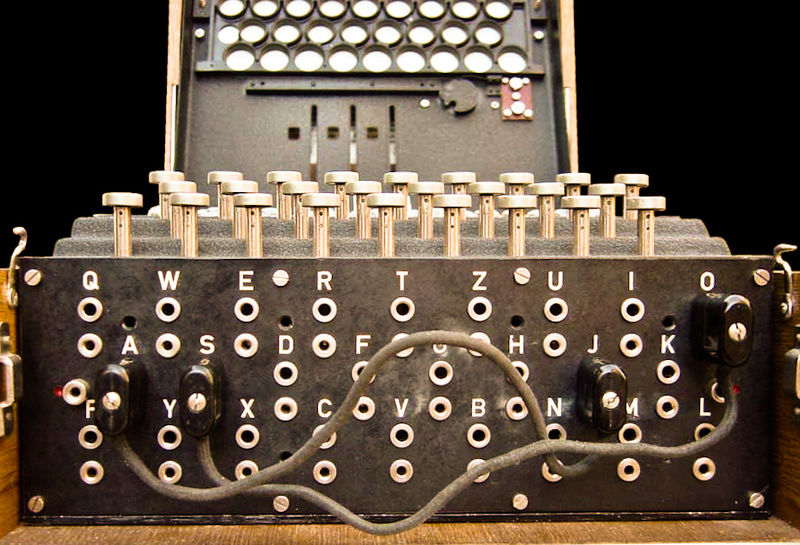
\includegraphics[scale=0.9]{images/plugboard.jpg}
%   \end{center}
%   \label{ref:plugboard}
%   \caption{Enigma \texttt{I} Plugboard}
% \end{figure}

Upon a key press, the electrical current corresponding to this letter
is sent to a mechanism known as the {\bf{plugboard}}. From an operator's
perspective, the plugboard was a series of ports, one for each
letter, along with 10 cables which could connect these ports. When
two letters are connected via a cable (e.g. A and Z), the plugboard
will send current corresponding to a letter to the opposite letter
(e.g. A goes to Z and vice versa). If no cable is plugged in to a
letter (e.g. D has no cable), then the plugboard simply will return a
current corresponding to this same letter (e.g. D). When a letter is connected to another 
through the plugboard, we will say that the letters are {\bf{steckered}} to one another. Assuming all 10
cables are used, this means that the plugboard can be represented as a
permutation on 26 letters with $2^{10}1^6$ cycle type\footnote{We
  will denote cycle types in this paper in the format
  $\lambda_1^{m_1}\dots\lambda_k^{m_k}$ where $\lambda_i$ is the length
of a cycle and $m_i$ is the multiplicity of this cycle length. We will often write the full notation $1^{m_1}\dots n^{m_n}$ in which $m_i$ may be $0$.}. One such
permutation could be
\begin{center}
  (\texttt{HR})(\texttt{AT})(\texttt{IW})(\texttt{SK})(\texttt{UY})(\texttt{DF})(\texttt{GV})(\texttt{LJ})(\texttt{BQ})(\texttt{MX})(\texttt{C})(\texttt{E})(\texttt{N})(\texttt{O})(\texttt{P})(\texttt{Z}).
\end{center}
In general, we will denote the permutation corresponding to a plugboard as $S$.

\subsection{The Rotors}
% \begin{figure}[htpb]
%   \centering
%   \begin{subfigure}{0.3\textwidth}
%     \includegraphics[width=\linewidth]{images/rotor_v_front.jpg}
%     \caption{Entry-side}
%     \label{fig:rotor_v_front}
%   \end{subfigure}
%   \hspace{0.02\textwidth}
%   \begin{subfigure}{0.3\textwidth}
%     \includegraphics[width=\linewidth]{images/rotor_v_back.jpg}
%     \caption{Exit-side}
%     \label{fig:rotor_v_back}
%   \end{subfigure}
%   \caption{Rotor \texttt{V}}
%   \label{fig:rotor_v}
% \end{figure}

The Enigma model \texttt{I} used three rotors, selected from a larger
set of rotors, the number of which changed depending on the military
branch we examine. At a minimum, all three branches of the military
had access to five rotors labeled by their roman numeral equivalents (i.e. $\texttt{I},\dots,\texttt{V}$).
Each rotor encoded a unique permutation from 26 input contacts to 26
output contacts by simply connecting between each input/output pair
in the permutation with a wire. The contacts represent the letters
in alphabetical order moving in a clockwise manner relative to the
entry side of the rotor. The input contacts of the rotor were often marked
with a white dot indicating which contact corresponded to \texttt{A},
but in general is found by looking at the contact immediately above
the numeral indicator.
\\\\On their own, these rotors would prove to be very poor
cryptographic devices, as they are just substitution ciphers, which are
vulnerable to frequency analysis and, if found by the enemy, would
serve no purpose whatsoever. Therefore, these rotors were designed to
rotate, which served to change the substitution at each stage of encryption.
\\\\Because these rotors rotate, it is best to differentiate between
contact letters and contact positions. When we give the permutation
corresponding to a rotor as in figure \ref{fig:rotor_v_wiring} we are
referring to the \texttt{A} contact as the specific contact denoted
by the marker dot and the \texttt{B} contact as its next contact
turning clockwise. When referred to in this context, we will use the
word ``contact''. On the other hand, when we say that an electrical
current corresponding to \texttt{A} enters a rotor, we mean
that the current enters the contact at the topmost \emph{position} of
the rotor, even if the rotor has rotated now so that that contact
is not the contact with the marker dot. When referred to in this
context we will use the word ``position'' so as to disambiguate from
the prior context. That is to say, a contact and a position need not
be the same. For example, contact \texttt{A} can be in position
\texttt{B}. This occurs when the pin with the marker dot adjacent to
it is one pin away from being at the top of the rotor.

\subsubsection{Turnover}
Each rotor had on its entry-side a notch next to each contact. A pawl
attempted to engage
the notch and move the rotor forward by one contact each key press.
On the exit-side, each
rotor was equipped with a smooth ring with only a single notch
breaking it. This is known as the {\bf{turnover notch}}. Assuming the
rotor functions in isolation the pawl will engage the entry notches
during each key press thus moving the rotor forward by one until,
after 26 presses, the rotor returns to its original position.
However, if we have two rotors, say rotor M and N, such that rotor M
has its entry contacts placed adjacent to the exit contacts of rotor
N; then, the smooth ring of the rotor N will occlude the notches of
rotor M thus preventing the pawl from engaging. That is, except at
the location where the turnover notch is located. The pawl will then
only be able to rotate rotor M if it aligns with the turnover notch of rotor N.
\\\\Now consider three rotors, rotors L, M, and N, arranged left to
right from an operator's perspective. Then electrical current first
enters rotor N, followed by rotor M, and finally rotor L. Rotor N
will have no rotor's smooth ring occluding its notches so the pawl is
free to engage rotor N at every key press. Thus rotor N will always
turn at each press of the key. Rotor M, however, will only turn at
the position at which rotor N's turnover notch aligns with the pawl
(save for a case we will shortly discuss),
meaning that for each full rotation of rotor N, rotor M will move
by one contact. Finally, rotor L will only move when rotor M's
turnover notch is aligned with the pawl, meaning that rotor N must make 26 full rotations before rotor L will move by one contact.

%% https://www.cryptomuseum.com/crypto/enigma/m3/index.htm %%
\begin{center}
  \begin{figure}[h]
    \[
      \left(
        \begin{array}{llllllllllllllllllllllllll}
          \texttt{A} & \texttt{B} & \texttt{C} & \texttt{D} &
          \texttt{E} & \texttt{F} & \texttt{G} & \texttt{H} &
          \texttt{I} & \texttt{J} & \texttt{K} & \texttt{L} &
          \texttt{M} & \texttt{N} & \texttt{O} & \texttt{P} &
          \texttt{Q} & \texttt{R} & \texttt{S} & \texttt{T} &
          \texttt{U} & \texttt{V} & \texttt{W} & \texttt{X} &
          \texttt{Y} & \texttt{Z}                             \\
          \texttt{V} & \texttt{Z} & \texttt{B} & \texttt{R} &
          \texttt{G} & \texttt{I} & \texttt{T} & \texttt{Y} &
          \texttt{U} & \texttt{P} & \texttt{S} & \texttt{D} &
          \texttt{N} & \texttt{H} & \texttt{L} & \texttt{X} &
          \texttt{A} & \texttt{W} & \texttt{M} & \texttt{J} &
          \texttt{Q} & \texttt{O} & \texttt{F} & \texttt{E} &
          \texttt{C} & \texttt{K}
        \end{array}
      \right)
    \]
    \caption{Rotor \texttt{V} permutation}
    \label{fig:rotor_v_wiring}
  \end{figure}
\end{center}

\subsubsection{Double Stepping}\label{double_step}
Arguably the most confusing aspect of the mechanics of the Enigma
machine is that of the {\bf{double step}}. We just said that the each
of the left two rotors ($M$ and $L$) can \emph{only} be moved when
the turnover notch of its right-hand adjacent rotor ($N$ and $M$
respectively) is aligned with the pawl. For $L$ this is true.
However, for rotor $M$, we must consider that even if rotor $N$'s
turnover notch is \emph{not} aligned with the pawl, rotor $M$'s own
turnover notch \emph{may} be aligned with the pawl. In this case, the
pawl will engage and move $L$; however, the turnover notch is still
connected to rotor $M$, so when the pawl engages $M$'s turnover notch
it will not only move $L$, but it will also move $M$ (just from the opposite side that we might expect).
\\\\We will illustrate this effect by example. Suppose our rotors
$N$, $M$, and $L$ had only three positions ($1$, $2$, and $3$). They
will each have a turnover notch aligned with a pawl when at position
$1$. We will walk through a full cycle of turnover of the leftmost
rotor $L$ step-by-step. We have
\begin{itemize}
  \item (Step $0$) $L = 2$, $M = 2$, $N = 3$ -- This represents our
    initial position
  \item (Step $1$) $L = 2$, $M = 2$, $N = 1$ -- Pawl engages $N$ and
    steps it forward
  \item (Step $2$) $L = 2$, $M = 3$, $N = 2$ -- Pawl engages $N$ and
    $N$'s turnover notch engages $M$.
  \item (Step $3$) $L = 2$, $M = 3$, $N = 3$ -- Pawl engages $N$ and
    steps it forward
  \item (Step $4$) $L = 2$, $M = 3$, $N = 1$ -- Pawl engages $N$ and
    steps it forward
  \item (Step $5$) $L = 2$, $M = 1$, $N = 2$ -- Pawl engages $N$ and
    $N$'s turnover notch engages $M$.
  \item (Step $6$) $L = 3$, $M = 2$, $N = 3$ -- Pawl engages $N$.
    $M$'s turnover notch engages $L$ but this also has the effect of
    rotating $M$ as well, even though $N$'s turnover notch is
    \emph{not} aligned. Observe that $M$ has now moved twice in two
    steps, hence the name ``double step''.
\end{itemize}
From this example, we note that on an Enigma with 26 letters, the leftmost rotor $L$
moves every $26\cdot25$ steps. We might expect this to occur every $26\cdot26$ steps, but
because of double stepping the period is shortened. 
\subsubsection{Rotation}

Consider the effect of a rotor turn on rotor \texttt{V}, whose
internal wiring is described in figure \ref{fig:rotor_v_wiring}.
In a default position in which contact \texttt{A} is at position
\texttt{A}. After pressing a key, the rotor
will turn resulting in contact \texttt{B} now being in position
\texttt{A}. This means that an input current
entering at position \texttt{A} will go into contact \texttt{B}, be
routed through the permutation and exit at contact
\texttt{Z} which now is at position \texttt{Y} due to the rotation.
This is to say that rotating the rotor has the effect
of shifting an input letter forward by 1 (mod 26) and the output
letter back by 1 (mod 26).
\\\\To encode the effect of rotation as a permutation consider
\begin{definition}
  The \emph{Caesar permutation} (denoted $P$) is the permutation
  taking a letter to the next letter in alphabetical order (mod 26).
  Its two-line permutation notation is
  \[
    \left(
      \begin{array}{llllllllllllllllllllllllll}
        \texttt{A} & \texttt{B} & \texttt{C} & \texttt{D} &
        \texttt{E} & \texttt{F} & \texttt{G} & \texttt{H} &
        \texttt{I} & \texttt{J} & \texttt{K} & \texttt{L} &
        \texttt{M} & \texttt{N} & \texttt{O} & \texttt{P} &
        \texttt{Q} & \texttt{R} & \texttt{S} & \texttt{T} &
        \texttt{U} & \texttt{V} & \texttt{W} & \texttt{X} &
        \texttt{Y} & \texttt{Z}                             \\
        \texttt{B} & \texttt{C} & \texttt{D} &
        \texttt{E} & \texttt{F} & \texttt{G} & \texttt{H} &
        \texttt{I} & \texttt{J} & \texttt{K} & \texttt{L} &
        \texttt{M} & \texttt{N} & \texttt{O} & \texttt{P} &
        \texttt{Q} & \texttt{R} & \texttt{S} & \texttt{T} &
        \texttt{U} & \texttt{V} & \texttt{W} & \texttt{X} &
        \texttt{Y} & \texttt{Z} & \texttt{A}
      \end{array}
    \right).
  \]
\end{definition}
If we denote the permutation corresponding to rotor \texttt{V} in
default position as $\eta$. Then after $r$ rotations, to get
our new permutation we must first shift each input letter forward by
$r$ and each output letter backwards by $r$. This can be encoded via
the Caesar permutation as follows
\[
  {P^{-r}}\eta{P^{r}}.
\]
\noindent It should be noted that current will only flow through the
machine \emph{after} the rotation has taken place. Thus encrypting a
letter with the window indicating \texttt{AAA} is really going to
send current through the rotors with the window indication
\texttt{AAB} since the rightmost rotor will turn before the encryption happens.
\subsubsection{Outer Ring}

The rotors were additionally equipped with an outer ring with
letters \texttt{A} to \texttt{Z} moving clockwise relative to the
entry-side of the rotor. Alternately some rings had numerical values
ranging from \texttt{01} to \texttt{26}. The outer ring was not fixed to the underlying rotor and could be moved. Most importantly, this outer ring is what contained the turnover notch. Thus by moving the outer ring we change where turnover occurs relative to the internal wiring of the rotor.
\\\\To consider the effect of this ring,
consider if an operator were instructed to place the ring such that
the outer ring's \texttt{02} label was placed over contact \texttt{A}. Once
the rotor is closed inside the machine
the operator can now only see the letters indicated by the outer ring
appearing in a small window. If he moves the ring's label \texttt{01}
to be in the window, then contact \texttt{Z} is now in position
\texttt{A}. This means that an input current
entering at position \texttt{A} will go into contact \texttt{Z}, be
routed through the permutation and exit
at contact \texttt{K} which now is at position \texttt{L} due to the
ring setting. This is to say that the moving the ring
setting has the effect of shifting an input letter back by 1 (mod 26)
and the output letter forward by 1 (mod 26).
As in the prior discussion on rotor rotation, if we denote the
permutation corresponding to rotor \texttt{V} in default position as
$\eta$. Then shifting the ring by $r$ letters, we get a new
permutation by first shifting each input letter backwards by $r$ and
each output letter forwards by $r$. This can be encoded via the
Caesar permutation as follows
\[
  {P^{r}}\eta{P^{-r}}.
\]
In this sense, we can think of rotor rotations and ring adjustments
as having inverse effects. In fact, if we ignore turnover, setting
the ring forward by $r$ letters and then rotating the rotor forward by $r$
letters is equivalent to having left the ring setting and rotor in
its default position. That is to say, for cases where turnover does
not occur, the ring setting (\emph{Ringstellung}) and which letter
we decide to show in our window (\emph{Grundstellung}) really
represent one singular component of our key space since we can always
consider our ring setting as being at \texttt{A} by just shifting
which letter we display in our window.
However, consider that changing the ring
setting also changes where the turnover occurs relative to the
internal wiring of a rotor. This means that for rotors $M$ and $L$
which are affected by turnover, the ring setting does add to
the key space since it has effects which are independent from the
window setting.

%% NOTE HAPPENES AFTER PAWL %%

% In default position the effect of this ring is just that it conveys
% which contact corresponds to which letter and, when the rotors are
% locked inside the Enigma machine, displays to the operator which
% letter is at the top of the rotor through a small window for each
% rotor. However, the ring itself was disconnected from the rotor and
% could be rotated freely. Further, the turnover notch moved along with
% the ring and thus changing the ring setting would also change the
% relative turnover point for each rotor.
% This has two effects.
% \begin{itemize}
%   \item If the operator is instructed to use rotor \texttt{V} and to
%         have \texttt{A} showing through the window on their machine then
%         if the ring setting is such that \texttt{A} on the ring
%         corresponds to contact letter \texttt{A} (the contact next to the
%         marker dot), then a current entering at the position
%         correpsonding to \texttt{A} will exit at the position
%         corresponding to \texttt{E}; however, if the ring setting is such
%         that \texttt{A} on the ring corresponds to contact letter
%         \texttt{B}, then a current entering at the position corresponding
%         to \texttt{A} will exit at the position corresponding to
%         \texttt{K} . In this sense the, ring setting has an inverse
%         relationship to how much the rotor has turned. If the rotor has
%         turned by one contact, but the ring setting has been turned by
%         one letter from the default position, then, as a permutation, it
%         is as if the rotor has a default ring setting and has not moved.
% \end{itemize}

\subsection{The Reflector}
After the current travels through all three rotors, it ends up at the
reflector which we will denote $R$. The reflector is specially
designed so that its permutation consists only of disjoint
transpositions, that is it has a $2^{13}$ cycle type. This means that
reflector simply swaps letters in a set of $13$ pairs.
\\\\Rather than having an entry and an exit side each with their own
contacts, the reflector has one side of contacts. Current enters at a
particular contact and is routed through the permutation back out
this same side at a different contact. The reason for this is that
the reflector's job is to send current through the exact inverse of
the process we have described up to this point. That is, after
exiting the reflector, current travels back through the rotors (now
entering at the exit contacts of the leftmost rotor), travels back
through the plugboard, and now ends up at a lamp light indicating the
enciphered letter.

\section{Key Size}

\subsubsection{\emph{Plugboard Setting (}Steckerverbindungen\emph{)}}
10 plugboard wires are selected in total. The first wire must connect
2 out of 26 letters giving us ${26\choose2}$ locations this wire can
be placed. We now select a wire for the next two letters giving us
${24\choose2}$ remaining locations. We continue in this fashion until
having placed 9 wires leaving us ${8\choose2}$ remaining choices. In
total, we have found
\begin{align*}
  & {26\choose2}{24\choose2}\dots{8\choose2}                                  \\
  & =\frac{26!}{2!\cdot 24!}\frac{24!}{2!\cdot 22!}\dots\frac{8!}{2!\cdot 6!} \\
  & =\frac{26!}{2^{10}\cdot6!}
\end{align*}
possible wire arrangements. Of course, the order in which we select
the 10 wires does not matter so we have over-counted and must
therefore divide this value by $10!$ wire orderings. Therefore, we have
\[
  \frac{26!}{2^{10}\cdot 10! \cdot 6!}
\]
plugboard settings.

\subsubsection{\emph{Rotor Selection (}Walzenlage\emph{)}}
From the 5 rotors in circulation, 3 rotors in some order were needed
to operate the Enigma machine. There are thus ${5}\choose{3}$ total
selections of 3 rotors each of which can be ordered in $3!$ ways,
giving us ${5\choose3}\cdot{3!}$ possibilities.

\subsubsection{\emph{Ring Setting (}Ringstellung\emph{)}}
Recall that the only rotors for which the ring setting actually adds
to the keyspace is the 2 rightmost rotors since this setting changes
where turnover occurs and only the 2 leftmost rotors are affected by
turnover. Since each ring can be setting corresponds a letter from
the 26 letter alphabet, this gives us $26^2$ possibilities.

\subsubsection{\emph{Window Setting (}Grundstellung\emph{)}}
A window setting specified 3 letters from the 26 letter alphabet
giving us $26^3$ possibilities.

\subsubsection{\emph{Reflector Selection}}
While there are multiple reflectors each of which saw varying levels
of usage during World War II, most machines generally stuck to a
fixed reflector known as \texttt{UKW-B}. Therefore, this does not
factor into our key space but is worth noting if other reflectors are
being considered.

\subsubsection{Total Key Size}
Putting together all these components of an Enigma's key settings we
derive the following expression for the total number of keys
\[
  \frac{26!}{2^{10}\cdot 10! \cdot 6!}\cdot{5\choose 3}\cdot3!\cdot
  26^2\cdot 26^3 \approx 1.07 \cdot 10^{23} \approx 2^{77}
\]
resulting in a roughly $77$-bit key space.
\\\\With such a large key space, it seemed to the Germans that Enigma
was unbreakable. This was an era before computers could churn through
massive key spaces in a matter of hours. Any attempt to break Enigma
was going to require an attack more intelligent than brute-forcing.
\\\\In Chapter 2, we will see how Polish cryptanalyst made use of a
flaw in the Enigma protocol, along with some clever mathematics, to
construct one of the earliest attempts at breaking the cipher. To
provide the requisite background, we will examine the protocol by
which German Enigma operators sent messages, as well as provide a
mathematical formalism for the machine.

\section{The Enigma Protocol}\label{protocol}
%% https://bletchleypark.org.uk/our-story/enigmas-of-bletchley-park/%%
%% https://www.cryptomuseum.com/crypto/enigma/i/index.htm%%
%% https://www.cryptomuseum.com/crypto/enigma/files/schluessel_m.pdf%^

%% FOR THE DATE GET
% chrome-extension://efaidnbmnnnibpcajpcglclefindmkaj/https://www.math.ias.edu/files/wam/rejewski.pdf
% $$
Suppose Alice and Bob are two radio operators (prior to September 15,
1938) who want to communicate securely. Each are supplied an Enigma
machine along with a key sheet indicating the keys for a given day.
The key sheet contains the following information:
\begin{itemize}
  \item the choice and order of rotors, known as the \emph{Walzenlage} -- at this point only three
      rotors \texttt{I}, \texttt{II}, and \texttt{III} were in
    production,
  \item the ring setting, known as the \emph{Ringstellung},
    %% See rejwinski for this %%
  \item the plugboard settings, known as the \emph{Steckerverbindungen} -- at this point only 3 jacks were used
    
  \item the window setting, known as the \emph{Grundstellung}.
\end{itemize}
A key sheet at this time may have looked along these lines.

\begin{figure}[H]
  \begin{center}
    \resizebox{0.98\textwidth}{!}{
      \begin{tabular}{|c|c|c|c|c|}
        \hline
        \textbf{\emph{\texttt{Datum}}}               &
        \textbf{\emph{\texttt{Walzenlage}}}          &
        \textbf{\emph{\texttt{Ringstellung}}}        &
        \textbf{\emph{\texttt{Steckerverbindungen}}} &
        \textbf{\emph{\texttt{Grundstellung}}}
        \\
        \hline
        \texttt{31.}                                 & \texttt{I II
        III}                                         & \texttt{10 14
        02}                                          & \texttt{BF SD
        AY}                                          & \texttt{VAR}
        \\
        \texttt{30.}                                 & \texttt{I II
        III}                                         & \texttt{04 25
        01}                                          & \texttt{UE PL
        AY}                                          & \texttt{PAQ}
        \\
        \texttt{29.}                                 & \texttt{I II
        III}                                         & \texttt{13 11
        06}                                          & \texttt{WJ VD
        PO}                                          & \texttt{ZJB}
        \\
        $\vdots$                                     & $\vdots$
        & $\vdots$      & $\vdots$ & $\vdots$ \\
        \hline
    \end{tabular}}
  \end{center}
  \caption{Mock Enigma Key Sheet pre-1938}
  \label{fig:keysheet_early}
\end{figure}

\noindent Alice wants to encrypt the message \texttt{HELLO WORLD} on
the 31st of the month using the key sheet in figure
\ref{fig:keysheet_early}. She opens the machine and places the rotors in
the machine from left to right as \texttt{I}, \texttt{II},
\texttt{III}\footnote{Prior to January 1, 1936, the sequence of
rotors was only changed once a quarter}. She then aligns the
\texttt{10} indicator on the
leftmost drum to be inline with the \texttt{A} contact, and similarly
for the remaining ring settings. Alice now closes the machine and
rotates the rotors so that they display \texttt{VAR} (or in numerals \texttt{22} \texttt{01} \texttt{18}) in the window of
each rotor. Finally, Alice connects \texttt{B} and \texttt{F} in the
plugboard and similarly for the remaining plugboard settings. Alice
now choose a random message key, this is a three letter trigram
called the \emph{Spruchschlüssel}. Alice chooses her message key as
\texttt{LSG} and is now ready to encrypt her message.
\\\\First, Alice will encrypt her message key \texttt{LSG} twice,
producing the hexagram
\begin{center}
  \texttt{KUW ACQ}
\end{center}
\noindent Alice now sets her window setting to her message key
\texttt{LSG} and begins enciphering her message \texttt{HELLO WORLD} to produce
\begin{center}
  \texttt{WQMYV HWGAB}
\end{center}
Alice now sends the following message to Bob
\begin{center}
  \texttt{KUW ACQ WQMYV HWGAB}
\end{center}
\noindent Bob recieves this message. He gets his key sheet and sets
up his machine as the key sheet describes for that day. He now types
in the first six letters of the message to get back Alice's message
key, which will look like
\begin{center}
  \texttt{LSG LSG}
\end{center}
We can now see why we doubly encoded the message key. If Bob did not
see the same trigram repeated twice he would know that either he or
Alice set up their machines incorrectly, or that Alice incorrectly typed in
her message key. Bob could then tell Alice to correct the message.
Now equipped with Alice's message key, Bob sets his machine window to
\texttt{LSG} and begins typing in the remainder of the message to
recover the plaintext
\begin{center}
  \texttt{HELLO WORLD}
\end{center}
\noindent It should be noted, the procedure described here is a
facsimile of the actual procedure meant to only convey the components
that are cryptographically significant. In practice, additional
information was sent alongside the message such as time of
transmission and radio station of origin. Further the message itself
was to be encoded with particular rules, for example, spaces would be
denoted with \texttt{X}. As we discuss changes to Enigma protocol
throughout this paper we will leave such details out.
%% https://www.ilord.com/enigma-manuals %%
%% REAL DECRYPT FOR EXAMPLE OH WAIT THESE MIGHT JUST BE TUNNY
% DECRYPTS
% https://web.archive.org/web/20160406042455/http://www.ilord.com/bp-decrypts.html
% %%
% Further, each have a copy of the ``\emph{Gebrauchsanleitung für die
% Chiffriermaschine Enigma}'' -- a book entailing all the protocols
% necessary for Alice
% and Bob to communicate securely. The manual explains
% \\\\\texttt{III. Setting the Key. }
% \\\texttt{10. The codebook issued with the machine determines the
% following 4 settings of the device:}
% \\\texttt{1. Order of the encryption rotors (III/IV, 12) (\emph{Walzenlage}),}
% \\\texttt{2. Setting of the number or letter rings( III/IV, 13) on
% the 3 encryption rotors (\emph{Ringstellung}),}
% \\\texttt{3. Setting of the numbers or letters visible in the
% windows (I/II, 16) (\emph{Grundstellung}),}
% \\\texttt{4. Establishment of the connections using the patchcords
% (II, 30) on the plug board (II, 15) (\emph{Steckerverbindungen}).}

%% FOR PROTOCOL NOTE FROM CODE BOOK TAHT CERTAIN SCRAMBLER POSITIONS
% WERE DISALLOWED YAY OR CERTAIN PLUGBOARD SETTINGS %%

\section{Enigma as a Permutation}

Recall that from the keyboard, current will enter the plugboard
($S$), followed by the rigtmost rotor ($N$), middle
rotor ($M$), leftmost rotor ($L$), and the reflector ($R$), only to
return through each of these components. Then at default position the
Enigma machine can be represented as a permutation
\[
  \sigma_0 \coloneq S^{-1}N^{-1}M^{-1}L^{-1}RLMNS
\]

\noindent Additionally recall that if we ignore turnover the ring setting and
window setting effectively represent one singular setting.
Then, by proper adjustment of permutations ($L$, $M$, and $N$) we can
consider any Enigma setting as beginning in such a state as described
by $\sigma_0$. Further, each subsequent key-press will bring us to a new
state with a new permutation given by
\[
  \sigma_i \coloneq S^{-1}P^{i}N^{-1}P^{-i}M^{-1}L^{-1}RLMP^{-i}NP^{i}S
\]
where $i$ describes the number of times we have depressed the
keyboard. Of course, turnover does exist and does matter; however, if
we are examining only the first few letters (say $l$) of a message
being encrypted, we have a $\frac{25}{26}$ chance of no turnover
occurring at each step and so we have a $(\frac{25}{26})^l$ chance of
no turnover occurring during our initial stages on encryption. For
small $l$ this is a reasonably high probability. We will see that the
first Enigma codebreakers made use of this
fact to simplify their model of the machine to the above permutation $\sigma_i$.

\subsection{Cycle Type}
Consider the structure of the permutation $\sigma_i$. We have
\begin{align*}
  \sigma_i & = S^{-1}P^{i}N^{-1}P^{-i}M^{-1}L^{-1}RLMP^{-i}NP^{i}S \\
  & = (LMP^{-i}NP^{i}S)^{-1}R(LMP^{-i}NP^{i}S).
\end{align*}
That is, $\sigma_i$ is simply the reflector permutation $R$
pre-composed and post-composed with a permutation and its inverse
respectively. This leads us to the following definition,

\begin{definition}
  Let $G$ be a group. We say two elements $a,b\in{G}$ are
  {\bf{conjugate}} if $\exists\text{ }g\in{G}$ s.t. $a=gbg^{-1}$.
\end{definition}
\text{}\\In this way, we can shorten our above observation to say that
$\forall\text{ }i\in\mathbb{N}$ we have that $\sigma_i$ and $R$ are
conjugate permutations. This point is true regardless of turnover since the permutations being pre-composed and post-composed with $R$ are always inverse permutations. Now consider the following lemma,\\
\begin{lemma}
  Suppose $\rho=(a_0\dots a_{k-1})\in S_n$ is a $k$-cycle. Then
  $\forall\text{ }\tau\in S_n$ we have
  $\tau\rho\tau^{-1}$ is a $k$-cycle.
  \label{conjugate_cycle}
\end{lemma}
\begin{proof}
  Since $\tau\in S_n$ is a bijection, to show how $\tau\rho\tau^{-1}$
  acts on $\{1,\dots, n\}$ it suffices to show how it acts on
  $\{\tau(1), \dots, \tau(n)\}$.
  We consider how $\tau\rho\tau^{-1}$ acts on elements of the form
  $\tau(a_i)$ for a fixed $i\in\{0,\dots,k-1\}$.
  \begin{align*}
    \tau(a_0\dots a_{k-1})\tau^{-1}(\tau(a_i)) & = \tau(a_0\dots
    a_{k-1})(a_i)
    \\
    & = \tau(a_{(i+1)\text{ mod }k}) \\
  \end{align*}
  Then we know $\tau\rho\tau^{-1}$ contains the cycle
  $(\tau(a_0)\dots \tau(a_{k-1}))$.
  Further, if $\tau\rho\tau^{-1}$ acts on the remaining elements
  $\tau(x)$ where $x\in\mathbb{N}_N - \{a_0,\dots,a_{k-1}\}$.
  Then we have
  \begin{align*}
    \tau(a_0\dots a_{k-1})\tau^{-1}(\tau(x)) & = \tau(a_0\dots a_{k-1})(x) \\
    & = \tau(x)                   \\
  \end{align*}
  Meaning $\tau\rho\tau^{-1}$ acts as the identity on $\tau(x)$. From
  this we can deduce that
  $\tau\rho\tau^{-1}$'s cycle decomposition consists of a single
  cycle of length $k$.
\end{proof}

\noindent This lemma leads us to the following theorem that will be of deep
relevance for the remainder of the paper.

\begin{theorem}
  \label{conjugate_cycle_type}
  $\forall\text{ }\alpha, \beta \in S_n$ we have
  \begin{center}
    $\alpha$ and $\beta$ are conjugates $\iff$ $\alpha$ and $\beta$
    have the same cycle type.
  \end{center}
\end{theorem}
\begin{proof}
\text{}\\$\Rightarrow$) Suppose $\exists\text{ }\tau\in S_n$ s.t.
$\alpha = \tau\beta\tau^{-1}$. $\beta$ has some cycle type
$1^{m_1}\dots n^{m_n}$. We can decompose
$\beta$ into disjoint cycles $\beta_{i,j}$ for $i\in\mathbb{N}_n$ and $j\in\mathbb{N}_{m_i}$. That is, there are $m_i$ cycles $\beta_{i,j}$ of length $i$. We then have,
\begin{align*}
  \alpha & = \tau\beta\tau^{-1}
  \\
  & = \tau\bigl(\beta_{1,1}\dots\beta_{1,m_1}\dots\beta_{n,1}\dots\beta_{n,m_n}\bigr)\tau^{-1}  \\
  & = \tau\beta_{1,1}(\tau^{-1}\tau)\dots(\tau^{-1}\tau)\beta_{1,m_1}(\tau^{-1}\tau)\dots(\tau^{-1}\tau)\beta_{n,1}(\tau^{-1}\tau)\dots(\tau^{-1}\tau)\beta_{n,m_n}\tau^{-1}  \\
    & = (\tau\beta_{1,1}\tau^{-1})\dots(\tau\beta_{1,m_1}\tau^{-1})\dots(\tau\beta_{n,1}\tau^{-1})\dots(\tau\beta_{n,m_n}\tau^{-1})  \\
\end{align*}
$\forall\text{ }i \in \mathbb{N}_n$ and $j \in \mathbb{N}_{m_i}$ we
have that $\beta_{i,j}$ is a cycle of length $i$ so
by Lemma \ref{conjugate_cycle} we have that $\tau\beta_{i, j}\tau^{-1}$ is an $i$ cycle.
\\\\Then to show $\alpha$ has cycle type
$1^{m_1}\dots n^{m_n}$ we need only show that each
$\tau\beta_{r, x}\tau^{-1}$ and $\tau\beta_{s,
y}\tau^{-1}$ are disjoint $\forall\text{ }r,s\in\mathbb{N}_n$ and
$x\in\mathbb{N}_{m_r}$, $y\in\mathbb{N}_{m_s}$ with $(r,x) \ne (s,y)$. Suppose not, that is
$\tau\beta_{r, x}\tau^{-1}$ and $\tau\beta_{s,
y}\tau^{-1}$ act non-fixedly on the same element. We write
$\beta_{r,x}$ as $(a_0\dots a_{r-1})$ and
$\beta_{s,y}$ as $(b_0\dots b_{s-1})$. These two
cycles are disjoint as they are independent cycles in the disjoint
cycle decomposition. Then $\forall\text{
}p\in\{0,\dots,r-1\}$ and $q\in\{0,\dots,s-1\}$ we
have that $a_p \ne b_q$.
We have from Lemma \ref{conjugate_cycle} that
\begin{align*}
  \tau\beta_{r, x}\tau^{-1} & = (\tau(a_0)\dots\tau(a_{r-1})) \\
  \tau\beta_{r, y}\tau^{-1} & = (\tau(b_0)\dots\tau(b_{s-1}))
\end{align*}
By supposition there must $\exists\text{ }\tau(a_p) = \tau(b_q)$;
However, we know $a_p \ne b_q$ and $\tau$ is an injection resulting in a
contradiction. Then $\alpha$ has cycle type
$1^{m_1}\dots n^{m_n}$.

\text{}\\$\Leftarrow$) Suppose $\alpha$ and $\beta$ both have cycle
type $1^{m_1}\dots n^{m_n}$. Then we can write $\alpha$ and $\beta$ as cycle decompositions into $m_i$ cycles of length $i$ as,
\begin{align*}
\alpha & = \prod_{i=1}^{n}\prod_{j=1}^{m_i}\alpha_{i,j}\\
\beta  & = \prod_{i=1}^{n}\prod_{j=1}^{m_i}\beta_{i,j}
\end{align*}
For $i\in\mathbb{N}_n$ and $j\in\mathbb{N}_{m_i}$, we can denote 
\begin{align*}
\alpha_{i,j} & = (a^{(i,j)}_0\dots a^{(i,j)}_{i-1})\\
\beta_{i,j}  & = (b^{(i,j)}_0\dots b^{(i,j)}_{i-1})
\end{align*}
Then we define $\tau:\mathbb{N}_n\to\mathbb{N}_n$ by 
\[
    \tau(b^{(i,j)}_k) = a^{(i,j)}_k
\] 
for any valid indices $i\in\mathbb{N}_n$, $j\in\mathbb{N}_{m_i}$, and $k\in\{0,\dots, i-1\}$.
We claim that $\alpha = \tau\beta\tau^{-1}$. We consider
$\tau\beta\tau^{-1}$'s action on some $a^{(i,j)}_k\in\mathbb{N}_n$.
Note that $a^{(i,j)}_k$ lies in some cycle of length $i$ and by
construction $b^{(i,j)}_k$ also lies in a cycle of length $i$.
\begin{align*}
\tau\beta\tau^{-1}(a^{(i,j)}_k) & = \tau\beta\tau^{-1}(\tau(b^{(i,j)}_k))        \\
& = \tau\beta(b^{(i,j)}_k)                       \\
& = \tau(b^{(i,j)}_{(k+1)\text{ mod }i}) \\
& = a^{(i,j)}_{(k+1)\text{ mod }i}      \\
& = \alpha(a^{(i,j)}_k)
\end{align*}
Since this is true for all $a^{(i,j)}_k$ and this covers all of $\mathbb{N}_n$, then we have $\alpha = \tau\beta\tau^{-1}$ and $\alpha$ and $\beta$ are conjugates.
\end{proof}
\begin{corr}\label{possible_conjugates}
Given $\alpha$ and $\beta$ of the same cycle type
$1^{m_1}\dots n^{m_n}$, there are
\[
\prod_{i=1}^{n}i^{m_i}m_i!
\]
permutations which conjugate $\alpha$ to $\beta$.
\end{corr}
\begin{proof}
We have seen via the above proof that permutations with conjugate
$\alpha$ to $\beta$ consist of mappings between the cycles of $\alpha$
and $\beta$ when cycles of the same length are written one over the
other. Of course, we can reorder the cycles of length $i$ in
$m_i!$ ways. Further, for each $i$ cycle (of which there are
$m_i$) we can shift each element up to $i$ times to get the
same permutation. This gives $i^{m_i}$ possible shifts of all $i$ cycles.
\end{proof}
\noindent This further gives us that, 
\begin{corr}\label{cycle_count}
    There are 
    \[
    \frac{n!}{\prod_{i=1}^n{i^{m_i}m_i!}}
    \]
    permutations with the cycle type $1^{m_1}\dots n^{m_n}$.
\end{corr}
\begin{proof}
Let $\alpha$ be any fixed permutation with cycle type $1^{m_1} \dots n^{m_n}$. Every permutation with this cycle type is a conjugate of $\alpha$. So, the number of such permutations is equal to the number of distinct conjugates of $\alpha$.
\\\\Every permutation $\pi \in S_n$ gives a conjugate $\pi \alpha \pi^{-1}$. However, different $\pi$ can produce the same permutation after conjugation. For two permutations $\pi$ and $\rho$ to produce the same permutation after conjugating $\alpha$ we must have 
\begin{align*}
&\pi\alpha\pi^{-1} = \rho\alpha\rho^{-1}\\
\Rightarrow\text{ }&\alpha = \pi^{-1}\rho\alpha\rho^{-1}\pi
\end{align*}
In other words, $\rho^{-1}\pi$ must conjugate $\alpha$ to $\alpha$
\\\\From the previous corollary, we know there are
\[
\prod_{i=1}^{n} i^{m_i} m_i!
\]
permutations conjugating $\alpha$ to $\alpha$.  
\\\\Then number of distinct conjugates of $\alpha$ — and therefore the number of permutations with the same cycle type — is
\[
\frac{n!}{\prod_{i=1}^n i^{m_i} m_i!}.
\]
\end{proof}
\noindent Returning to the Enigma, recall that at any fixed position of the Enigma machine, the
permutation describing this position $\sigma_i$ is just a conjugate
of the reflector permutation $R$. As the reflector permutation $R$ has a cycle type
of $2^{13}$ it must then be the case by Theorem
\ref{conjugate_cycle_type} that at any given position the Enigma
machine is simply a $2^{13}$ cycle. This gives two key properties at
any given fixed position:
\begin{itemize}
\item[(1)] The Enigma is an involution, meaning that $\sigma_i(\sigma_i(x))
= x$. This is actually a desired and arguably necessary property for
the Enigma to work since we need to ensure that, when two
machines are at the same position, a cipher letter $\sigma_i(x)$ will
decrypt to its plain-text counterpart $x$.
\item[(2)] The Enigma has no fixed points. Since $\sigma_i$ is composed of
13 disjoint transpositions, we can never have a letter $x$ for which
$\sigma_i(x) = x$. Therefore, we will never see a letter encrypted to
itself. This means that for \emph{any} setting, repeatedly pressing a letter (e.g. $\texttt{A}$) on an Enigma machine
 will \emph{never} produce the same letter
(e.g. $\texttt{A}$) on the output bulbs.
\end{itemize}
% \\\begin{figure}[h]
%   \begin{center}
%     \resizebox{0.98\textwidth}{!}{
% \begin{tabular}{|c|c|c|c|c|}
% \hline
% \textbf{\emph{\texttt{Datum}}} &
% \textbf{\emph{\texttt{Walzenlage}}} &
% \textbf{\emph{\texttt{Ringstellung}}} &
% \textbf{\emph{\texttt{Steckerverbindungen}}} &
% \textbf{\emph{\texttt{Grundstellung}}} \\
% \hline
% \texttt{31.} & \texttt{IV II I} & \texttt{F T R} & \texttt{HR AT IW
% SK UY DF GV LJ BQ MX}   & \texttt{sfy azy zkq bqi} \\
% \texttt{30.} & \texttt{III V II} & \texttt{Y V P} & \texttt{OR KI
% JV }   & \texttt{iuy swz omo myj} \\
% \texttt{29.} & \texttt{V IV I} & \texttt{O H R} & \texttt{WJ VD PO
% MQ FX ZR NE LG UO BK}   & \texttt{rui kao fqi rwu} \\
%   $\vdots$ & $\vdots$ & $\vdots$ & $\vdots$ & $\vdots$ \\

% \hline
% \end{tabular}}
% \end{center}
%   \caption{Example Enigma Key Sheet (September 1938)}
%   \label{fig:enigma_key_sheet}
% \end{figure}
%% https://www.researchgate.net/figure/Enigma-key-book-Photo-from-authentic-German-codebook-From-before-September-1938-as-it_fig2_339932418
% %%

% \\\begin{figure}[h]
%   \begin{center}
%     \resizebox{0.98\textwidth}{!}{
% \begin{tabular}{|c|c|c|c|c|}
% \hline
% \textbf{\emph{\texttt{Datum}}} &
% \textbf{\emph{\texttt{Walzenlage}}} &
% \textbf{\emph{\texttt{Ringstellung}}} &
% \textbf{\emph{\texttt{Steckerverbindungen}}} &
% \textbf{\emph{\texttt{Kenngruppen}}} \\
% \hline
% \texttt{31.} & \texttt{V II IV} & \texttt{17 09 02} & \texttt{KT AJ
% IV UR NY HZ GD XF PB CQ}   & \texttt{sfy azy zkq bqi} \\
% \texttt{30.} & \texttt{I III V} & \texttt{22 12 10} & \texttt{UE PL
% AY TB ZH WM OJ DC KN SI}   & \texttt{iuy swz omo myj} \\
% \texttt{29.} & \texttt{V IV II} & \texttt{04 01 25} & \texttt{WJ VD
% PO MQ FX ZR NE LG UO BK}   & \texttt{rui kao fqi rwu} \\
% \texttt{28.} & \texttt{II III IV}  & \texttt{05 03 12} & \texttt{HR
% TJ LD IO CN GX QK PZ WS AF}   & \texttt{ioy kjv yko fpz} \\
% $\vdots$ & $\vdots$ & $\vdots$ & $\vdots$ & $\vdots$ \\
% \hline
% \end{tabular}}
% \end{center}
%   \caption{Mock Enigma Key Sheet for April 1943.}
%   \label{fig:enigma_key_sheet}
% \end{figure}

% LocalWords:  plugboard

\chapter{The Polish Bomba}
%% https://www.cryptocellar.org/pubs/ukwa.pdf%%
%% https://www.cryptocellar.org/enigma/files/rejewski-paper.pdf %% 

Rejewski was saddled with arguably the most complex discoveries in Enigma code breaking. Not only did he need to determine a means to recover daily keys from limited intellegence supplied by ?? but he additionally needed to recover the wirings of the rotors themselves.
\section{Characteristics}
Rejewksi quickly determined the protocol by which messages were enciphered -- in fact, he stated the this protocol was ``obvious.'' We will see that purely with knowledge of this procudure and some military intellegence, Rejewski was able to determine the rotor wirings necessary to make further cryptanalysis possible.
\\\\Consider the first six letters transmitted according to our encryption producedure. Operator Alice has some three letter private key (say \texttt{XYZ}) which she encodes twice with the machine settings specified by her key sheet. This will give us six encrypted letters $\sigma_1(\texttt{X})\sigma_2(\texttt{Y})\sigma_3(\texttt{Z})\sigma_4(\texttt{X})\sigma_5(\texttt{Y})\sigma_6(\texttt{Z})$. Suppose these six letters are given as
\begin{center}
	\texttt{ABC} \texttt{DEF}
\end{center}
That is
\begin{align*}
	\sigma_1(\texttt{X}) & = \texttt{A} \\
	\sigma_2(\texttt{Y}) & = \texttt{B} \\
	\sigma_3(\texttt{Z}) & = \texttt{C} \\
	\sigma_4(\texttt{X}) & = \texttt{D} \\
	\sigma_5(\texttt{Y}) & = \texttt{E} \\
	\sigma_6(\texttt{Z}) & = \texttt{F} \\
\end{align*}
Since each $\sigma_i$ is represented by 13 disjoint transpositions we can deduce, for example, that
\[
	\sigma_1\sigma_4(D) = \sigma_1(X) = A.
\]
With a sufficient set of hexagrams from gathered messages, we could then fully deduce the permutation $\sigma_1\sigma_4$. Further, we could recover $\sigma_2\sigma_5$ and $\sigma_3\sigma_6$. Rejewski refered to these paired permutations as {\bf{characteristics}}. In practice, such recovered characteristics may look like
\begin{align*}
	\sigma_1\sigma_4 & = (\texttt{DVPFKXGZYO})(\texttt{EIJMUNQLHT})(\texttt{BC})(\texttt{RW})(\texttt{A})(\texttt{S}) \\
	\sigma_2\sigma_5 & = (\texttt{BLFQUEOUM})(\texttt{HJPSWIZRN})(\texttt{AXT})(\texttt{CGY})(\texttt{D})(\texttt{K}) \\
	\sigma_3\sigma_6 & = (\texttt{ABVIKTJGFCQNY})(\texttt{DUZREHLXWPSMO})
\end{align*}
Rejewski noted a key structural similarity between all such characteristics recovered in this fashion: in each characteristic, cycles of the same length appear in pairs.
\\\\To see why this happens consider the following lemma,
\begin{lemma}
	\label{cillies}
	Suppose $(\alpha\beta)$ appears in $\sigma_i$ for $i\in\{1,2,3\}$. Then $\alpha$ and $\beta$ will appear in disjoint cycles of $\sigma_i\sigma_{i+3}$ of equal length.
\end{lemma}
\begin{proof}
	%% chrome-extension://efaidnbmnnnibpcajpcglclefindmkaj/https://www.math.ias.edu/files/wam/rejewski.pdf %%
	We begin by noting that if $(\alpha\beta)$ is in $\sigma_{i+3}$ then $\pi$ contains fixed points at $\alpha$ and $\beta$ and our claim is true. Then without loss of generality we can arrange $\sigma_{i}$ and $\sigma_{i+3}$ (non-exhaustively) in the following way:
	\[
		\setlength{\arraycolsep}{15pt}
		\begin{array}{cc}
			\sigma_i      & \sigma_{i+3} \\
			\hline
			(\alpha\beta) & (\beta x_1)  \\
			(x_1 x_2)     & (x_2 x_3)    \\
			\vdots        & \vdots       \\
			(x_{k-1} x_k) & (x_k \alpha)
		\end{array}
	\]
	Then the product $\sigma_i\sigma_{i+3}$ will be
	\[
		\sigma_1\sigma_{i+3} = (\alpha x_1 x_3 \dots x_{k-1} )(x_k x_{k-2} \dots x_2 \beta)
	\]
	and thus $\alpha$ and $\beta$ end up in disjoint cycles of equal length.
\end{proof}

This lemma has several consequences.
\begin{itemize}
	\item A characteristic like $\sigma_1\sigma_4$ which has two singletons $\texttt{A}$ and $\texttt{S}$ (in this context they are refered to as {\bf{females}}) then both $\sigma_1$ and $\sigma_4$ must have the transposition $(\texttt{AS})$.
	\item A characteristic like $\sigma_3\sigma_6$ (two disjoint 13 cycles) reduces the space of possible $\sigma_3$'s to just 13 permutations which will take the form
	      \begin{center}
		      $(\texttt{AD})(\texttt{BO})(\texttt{VM})\dots(\texttt{YU})$ \\
		      $(\texttt{AU})(\texttt{BD})(\texttt{VO})\dots(\texttt{YZ})$ \\
		      $\vdots$                                       \\
		      $(\texttt{AO})(\texttt{BM})(\texttt{VS})\dots(\texttt{YD})$
	      \end{center}
	      and similarly for $\sigma_6$.
\end{itemize}
Thus with absolutely no knowledge of the rotor wirings or the daily key, we can already tractibly compute a searchable space of $\sigma_i$'s. To determine which $\sigma_i$ is the correct one, we make use of the most prevalent bug in cryptography -- operator error.

\subsection{Cillies}
Enigma operators were instructed to construct random trigrams for their message keys -- likely to prevent frequency analysis attacks on the hexagrams beginning messages; However, operators often chose the same trigrams for each message. Some examples might inclide
\begin{itemize}
	\item Initials or first letters of the operator's spouse. For example, \texttt{CIL} perhaps deriving from the name ``Cecelia'' being shortened to ``cillie''. Allegadely for this reason, poor selections of trigrams from operators became known as {\bf{cillies}}.
	\item The same letter encoded three times such as \texttt{JJJ}
	\item Locations such as \texttt{LON} representing London.
	\item Later, Bletchley Park cryptanalyst John Herivel noticed that many operators selected message keys that were very close to the provided ring settings potentially allowing for a quick means of determining the ring settings.

	      %% Battle of wits the complete story of codebreaking in World War II PAGE 143 %% 
\end{itemize}
By keeping track of various radio stations which used cillies. Rejewski had a reasonable guess as to what the message key used for a particular ciphertext were. Suppose we recieved three hexagrams originating from a radio station which often used \texttt{JJJ} as their message key:
\begin{center}
	\texttt{SUG SMF}\\
	\texttt{SJM SPO}\\
	\texttt{SYX SCW}.
\end{center}

We can then compare these message keys against our possibilites for $\sigma_i$s to determine if $\texttt{JJJ}$ could have in fact been used to encipher these hexagrams. For example, the first hexagram could not have been used since \texttt{J} and \texttt{G} lie in the same cycle of $\sigma_3\sigma_6$ which would contradict lemma \ref{cillies}. Contiuing in this fashion we may hypothesize that the third hexagram was likely an enciphering of the repeated letter $\texttt{J}$.
\\\\To confirm this hypothesis we can use the supposition to further reduce the possible $\sigma_i$s. In fact, in our case, such a hypothesis would completely determine which $\sigma_3$ and $\sigma_6$ were being used and for the remaining $\sigma_i$s we are only left with a small set of options. We can then confirm our hypothesis by trying such $\sigma_i$s on hexagrams from other radio stations suspected of using cillies. If we find that $\texttt{PPP}$ is the message key corresponding to our deduced $\sigma_i$s we have reason to believe that our initial hypothesis was correct. If our hexagram corresponded to a key \texttt{PPA} we may only need to select a new choice of possible $\sigma_i$s to instead produce the expected cilly. In this way, we can recover each $\sigma_i$ and thus recover any transmission's message key -- all without any knowledge of internal wirings, plugboard settings, or daily keys.
\section{Wiring Recovery}

Equipped with a means to determine each $\sigma_i$, Rejewski set himself to finding the internal wirings of the rotors. The full recovery of rotor wirings and turovers is out of scope of this paper; However, we will provide a brief description to illustrate that with minimal intellegence information, entire rotor wirings were able to be deduced.
\\\\We begin by expanding $\sigma_i$ to
\[
	\sigma_i = S^{-1}P^{-(x+i)}N^{-1}P^{x+i}M^{-1}L^{-1}RLMP^{-(x+i)}NP^{x+i}S
\]
where $x$ accounts for the initial starting position of the rightmost rotor.
Since $M^{-1}L^{-1}RLM$ does not change between $\sigma_i$s we will denote this permutation $Q$ thus simplifying our earlier expression to
\[
	\sigma_i = S^{-1}P^{-(x+i)}N^{-1}P^{x+i}QP^{-(x+i)}NP^{x+i}S
\]
Rejewski knew the plugboard settings for two whole months, so he began shifting knowns and unknowns to opposite sides. Shifting things around gives us
\begin{align*}
	                    & \sigma_i = S^{-1}P^{-(x+i)}N^{-1}P^{x+i}QP^{-(x+i)}NP^{x+i}S     \\
	\Rightarrow\text{ } & S\sigma_i S^{-1} = P^{-(x+i)}N^{-1}P^{x+i}QP^{-(x+i)}NP^{x+i}    \\
	\Rightarrow\text{ } & P^{(x+i)}S\sigma_i S^{-1}P^{-(x+i)} =  N^{-1}P^{x+i}QP^{-(x+i)}N
\end{align*}
To further simplify notation we will then define ${\rho_i} \coloneq P^{(x+i)}S\sigma_i S^{-1}P^{-(x+i)}$. Then we have now have
\[
	\rho_i = N^{-1}P^{x+i}QP^{-(x+i)}N
\]
where $\rho_i$s are known from the key sheets Rejewski had access to. We will now eliminate this equations dependence on $Q$ by considering pairs of $\rho_i$ and $\rho_{i+1}$
\begin{align*}
	\rho_i\rho_{i+1} & = N^{-1}P^{x+i}QP^{-(x+i)}NN^{-1}P^{x+i+1}QP^{-(x+i+1)}N \\
	                 & = N^{-1}P^{x+i}QP^{-(x+i)}P^{x+i+1}QP^{-(x+i+1)}N        \\
	                 & = N^{-1}P^{x+i}QPQP^{-(x+i+1)}N                          \\
	                 & =N^{-1}P^{x+i}(QPQP^{-1})P^{-{x+i}}N
\end{align*}
Each $\rho_i\rho_{i+1}$ shares the common subexpression $QPQP^{-1}$. We can eliminate this subexpression by noting
\begin{align*}
	\rho_{i+1}\rho_{i+2} & = N^{-1}P^{x+i+1}(QPQP^{-1})P^{-{x+i+1}}N                                                     \\
	                     & = N^{-1}P^{x+i+1}(P^{-(x+i)}NN^{-1}P^{x+i})(QPQP^{-1})(P^{-(x+i)}NN^{-1}P^{x+i})P^{-{x+i+1}}N \\
	                     & = N^{-1}P^{x+i+1}P^{-(x+i)}N(N^{-1}P^{x+i}QPQP^{-1}P^{-(x+i)}N)N^{-1}P^{x+i}P^{-{x+i+1}}N     \\
	                     & = N^{-1}P^{x+i+1}P^{-(x+i)}N(\rho_i\rho_{i+1})N^{-1}P^{x+i}P^{-{x+i+1}}N                      \\
	                     & = N^{-1}P^{-1}N(\rho_i\rho_{i+1})N^{-1}PN                                                     \\
\end{align*}
We now have a relationship between each $\rho_i\rho_{i+1}$ and $\rho_{i+1}\rho_{i+2}$ by conjugating by $N^{-1}PN$. Now recall from theorem \ref{IDK} that if $\rho_i\rho_{i+1}$ has a reasonbaly large cycle structure, then there are only a limited number of possible permutations for $N^{-1}PN$. The relationship between $\rho_{i+1}\rho_{i+2}$ and $\rho_{i+2}\rho_{i+3}$ will further reduce these possibilities since of course $N^{-1}PN$ must be the same between these two relationships. Eventually, we can fully deduce $N^{-1}PN$. Finally, this will give us $26$ possibilites for $N$ representing its $26$ intial starting positions, and thus we can recover $N$ itself representing the internal wiring of the rigthmost rotor.
\\\\In a similar fashion we can recover the remaining rotor wirings though often with the help of other mathematical tricks, not to mention military intellegence and luck. From this point forward, we will assume that the cryptanalyst now has access to the wirings of all the rotors as well as the reflector.

\section{The Grill Method}

We now have deduced all of the rotors $N$, $M$, $L$, $R$ and each $\sigma_i$. We will use this information to recover the daily keys. For the moment, let us assume $S$ is the identity permutation. Then rearranging $\sigma_i$ we get
\begin{align}
	Q = P^{-(x+i)}NP^{x+i}\sigma_iP^{-(x+i)}N^{-1}P^{x+i} \label{eq:q_eq}
\end{align}
Since $Q$ must be the same for each such equation involving $\sigma_i$ we will devise a manual way to deduce $Q$. We can precompute $N$, $P^{-1}NP$, $\dots$, $P^{4}NP^{-4}$ and arrange them in a large sheet called the {\bf{bottom sheet}}.
Then for each $\sigma_i$ we can write out $\sigma_i$ with a slit beneath it to allow space for each possible $P^{-k}NP^k$. We will illustrate this for $\sigma_1$ and denote the spaces beneath with periods.
\begin{align*}
	\texttt{|}          & \texttt{ABCDEFGHIJKLMNOPQRSTUVWXYZ} \texttt{|} \\
	\sigma_1\texttt{ |} & \texttt{SRWIVHNFDOLKYGJTXBAPZECQMU} \texttt{|} \\
	\texttt{|}          & \texttt{..........................} \texttt{|}
\end{align*}
We will call this the {\bf{top sheet}}. By sliding the bottom sheet beneath the top sheet we can test various values of $P^{-k}NP^{k}$ to see what values of $Q$ they give. For example, for $k = 0$ we have
\begin{align*}
	\texttt{|}          & \texttt{ABCDEFGHIJKLMNOPQRSTUVWXYZ} \texttt{|} \\
	\sigma_1\texttt{ |} & \texttt{SRWIVHNFDOLKYGJTXBAPZECQMU} \texttt{|} \\
	N \texttt{ |}       & \texttt{KJPZYDTIOHXCSGUBRNWFMVEQLA} \texttt{|}
\end{align*}
We know that $Q(\texttt{A}) = (P^{-k}NP)\sigma_i(P^{-k}NP)^{-1}(\texttt{A})$. Therefore to compute $Q(\texttt{A})$ we first begin at $\texttt{A}$ in our bottom row to find that $N^{-1}(\texttt{A})=\texttt{Z}$. We now map $\texttt{Z}$ through $\sigma_i$ by finding $\texttt{Z}$ on the top row and seeing where it lands in the middle row, thus giving $\sigma_iN^{-1}(\texttt{A}) = \texttt{U}$. Finally to see where $N$ maps $\texttt{U}$ by finding $\texttt{U}$ on the top row and seeing where it lands in the middle row, thus giving $Q(\texttt{A}) = N\sigma_iN^{-1}(\texttt{A}) = M$. Continuing in this fashion we can get a candidate $Q$ generated by the guess that $\sigma_i$ aligned with $N$ in the sheet. Recall that $Q$ must be consistent between each equation \ref{eq:q_eq}. To check this we can simply construct our top sheet so that each $\sigma_i$ is placed over one another each with a slot beneath it. We can now get candidate $Q$s for each $\sigma_i$. If we find that our offset of the bottom sheet creates inconsistencies we can move the bottom sheet up by one until we find candidates that are consistent between each $\sigma_i$.
\\\\If $S$ were truly the identity then we would ultimately find an offset that generates identical $Q$s for each $\sigma_i$. Of course, $S$ will not be the identity. Thus, instead of looking for perfect consistency between each $Q$ we are only looking for relative consistency between each $Q$ where perhaps a majority send one letter to another. By comparing $Q$s generated by each $\sigma_i$ we can deduce with reasonable certainty the value of the true $Q$ by just considering where the majority of the $Q$s map \texttt{A}, \texttt{B}, and so on. Further, the offset in the bottom sheet which generated the most consistent permutations $Q$ will give us the offset of the rightmost rotor. Additionally, using this method, we can see where the $Q$s fail to line up to determine which letters are steckered and which are unsteckered, along with some of the steckerings themselves. Such a method was called the {\bf{grill method}} and required tedious work and had many possibilites for mistakes.
\\\\To determine the offsets of the remaining two rotors we can simply enumerate all $26^2 = 676$ positions of the left two rotors (for both possible orderings of the rotors) until $Q$ is produced. In practice, a catalogue was eventually compiled which associated each $Q$ to a corresponding position and ordering of the left two rotors. Now equipped with each rotor position, we still must determine the ring settings.
\\\\To determine the ring settings we make use of another operator error. Often messages began with the letters \texttt{ANX} which is the German word ``to'' along with \texttt{X} denoting a space. We could therefore set the ring setting to its default lcoation and then brute force all $26^3$ possible rotor positions until the first letters in the deciphered message were \texttt{ANX}. Once we knew the position at which this occured, along with the message key, we can immediately determine what the ring settings must have been to produce this message -- since the ring setting and rotor position have inverse effects on the rotor permutation.

\section{The Clock Method}

At this point Rejewski and his team were able to recover daily keys, but the above methods are extremely slow and inefficient. Many optimizations were made over the years. We will now examine one particular optimization.
\\\\While we do know the wirings of the rotors, we do not know when we begin our cryptanalysis what the order of these rotors were. At the time there were only three rotors in use (\texttt{I}, \texttt{II}, \texttt{III}) so one could simply try all 3 rotors as the rightmost one and repeat the above analysis. Of course, this makes the above method 3 times slower. In practice, early Enigma daily keys kept rotor positions the same for an entire 3 month period meaning this analysis did not need to be done too frequently.
\\\\However, Jerzy Różycki worked out an efficient method to determine the rightmost rotor which he called the {\bf{clock method}}. The clock method attempted to determine where the turnover notch was for the rightmost rotor. From this we could immediately determine which of the three rotors was used.

\subsection{Index of Coincidence}
In a string of random text from a 26 letter alphabet we get a uniform distribution of letters. However, text which encodes a language does not generate a uniform distribution. Distributions for various languages have been well studied and are the information needed for frequency analysis. Having a non-uniform distribution also implies that when we align two pieces  of text which encodes a language (call them $\texttt{T}_A$ and $\texttt{T}_B$), the chance that a letter from $\texttt{T}_A$ will align at the same position with a letter from $\texttt{T}_B$ is non-uniform. We can therefore detect if  $\texttt{T}_A$ and $\texttt{T}_B$ are encoded with the same polyalphabetic cipher by counting the number of aligned letters between them (called {\bf{coincidences}}) and seeing if they represent a non-uniform frequency.
\\\\To make use of this property, we can select two messages with message keys whose first two letters coincided (e.g. \texttt{XYA} and \texttt{XYF}). This meant that both messages were encoded with the only difference being in their rightmost rotor. If at some point during encoding the first message, its rotors align with the rotors used to encode the second message, we would expect to see the number of coincidences between the messages to suddenly spike significantly, in this way, we can detect when the two messages had their rotors align. This does not work, however, if turnover occurs then the two messages will not align in their rotor positions and we will see a random distribution of coincidences. If we align the message generated by $\texttt{XYA}$ on top of the message generated by $\texttt{XYF}$ we can slide the bottom message until is 5 positions further than the top message,
\begin{align*}
	 & \texttt{XYA}: \texttt{PASLK XASSP AUSDK XPVNW UULVT LWKRE KGUQO DSUKV ZOLMZ ZHYBF}                                                                                                                                                      \\
	 & \texttt{XYF}: \texttt{ }\texttt{ }\texttt{ }\texttt{ }\texttt{ }\texttt{ }\texttt{BAWXV ETTOP JZHXL VWGGQ MWDII OEHQO YSLRB IYLGB CHBYT }                                                                                               \\
	 & \ \ \ \ \ \ \ \ \ \ \ \ \ \ \ \ \ \ \texttt{*}\ \ \ \ \ \ \ \ \ \ \ \ \ \ \ \ \ \ \ \ \ \ \ \ \ \ \ \ \ \ \ \ \ \ \ \ \ \texttt{*}\ \ \ \ \ \ \ \ \ \ \ \texttt{**}\ \ \ \texttt{*}\ \ \ \ \ \ \ \ \ \texttt{*}\ \ \ \ \ \ \ \texttt{*}
\end{align*}
at this point we would expect the texts to both be encoded by $\texttt{XYF}$ and the number of coincidences (indicated by \texttt{*}) should spike as we see in the above diagram. If this does not occur, this means no turnover occured between $\texttt{A}$ and $\texttt{F}$. This, for example, eliminates rotor \texttt{II} as a candidate since its turnonver occurs when \texttt{E} is displayed in the window. We can gain further information by performing the above procecdure but now with the message encoded by $\texttt{XYF}$ on the top and the message encoded by $\texttt{XYA}$ on the bottom. In this way we can determine which rotor was being used. The clock method was a precursor to a method we will discuss later known as Banburismus. The important takeaway is that language frequency analysis may not be strong enough to decode Enigma messages, it may be strong enough to determine elements of the key like rotor choice or ordering.

\section{The Cyclometer}

These manual methods of decryption became increasingly difficult as German operators were instructed to use more plugboard jacks and increased the rate at which daily keys changed. Rejewski wanted to produce a mechanical means of performing a similar deduction. He returned to the characteristics associated with a particular day's key. He noticed that the cycle structure of a characteristic did not regularly repeat (if at all). Then we perhaps could create a ``fingerprint'' of a key by noting the cycle structure of all three characteristics associated to the key. Now that Rejewski had the internal rotor wirings, he could build a machine that could immediately produce the cycle structure of characteristics for a given setting.
\\\\Let us first understand the manual implementation of such a deduction. Assuming an identity plugboard $S$ we can use our internal rotor wirings to know the exact permutaition $\sigma_1$ and $\sigma_3$ for any initial rotor position. In specific, suppose we have

\begin{center}
	\[
		\left(
		\begin{array}{llllllllllllllllllllllllll}
				\texttt{A} & \texttt{B} & \texttt{C} & \texttt{D} &
				\texttt{E} & \texttt{F} & \texttt{G} & \texttt{H} &
				\texttt{I} & \texttt{J} & \texttt{K} & \texttt{L} &
				\texttt{M} & \texttt{N} & \texttt{O} & \texttt{P} &
				\texttt{Q} & \texttt{R} & \texttt{S} & \texttt{T} &
				\texttt{U} & \texttt{V} & \texttt{W} & \texttt{X} &
				\texttt{Y} & \texttt{Z}                             \\
				\texttt{P} & \texttt{T} & \texttt{K} & \texttt{X} &
				\texttt{R} & \texttt{Z} & \texttt{Q} & \texttt{S} &
				\texttt{W} & \texttt{M} & \texttt{C} & \texttt{O} &
				\texttt{J} & \texttt{Y} & \texttt{L} & \texttt{A} &
				\texttt{G} & \texttt{E} & \texttt{H} & \texttt{B} &
				\texttt{V} & \texttt{U} & \texttt{I} & \texttt{D} &
				\texttt{N} & \texttt{F}
			\end{array}
		\right)
	\]
	$\sigma_1$
\end{center}
\begin{center}
	\[
		\left(
		\begin{array}{llllllllllllllllllllllllll}
				\texttt{A} & \texttt{B} & \texttt{C} & \texttt{D} &
				\texttt{E} & \texttt{F} & \texttt{G} & \texttt{H} &
				\texttt{I} & \texttt{J} & \texttt{K} & \texttt{L} &
				\texttt{M} & \texttt{N} & \texttt{O} & \texttt{P} &
				\texttt{Q} & \texttt{R} & \texttt{S} & \texttt{T} &
				\texttt{U} & \texttt{V} & \texttt{W} & \texttt{X} &
				\texttt{Y} & \texttt{Z}                             \\
				\texttt{J} & \texttt{W} & \texttt{V} & \texttt{R} &
				\texttt{O} & \texttt{S} & \texttt{U} & \texttt{Y} &
				\texttt{Z} & \texttt{A} & \texttt{T} & \texttt{Q} &
				\texttt{X} & \texttt{P} & \texttt{E} & \texttt{N} &
				\texttt{L} & \texttt{D} & \texttt{F} & \texttt{K} &
				\texttt{G} & \texttt{C} & \texttt{B} & \texttt{M} &
				\texttt{H} & \texttt{I}
			\end{array}
		\right)
	\]
	$\sigma_3$
\end{center}
Then to find the permutation $\sigma_1\sigma_3$ we might do the following. We begin with \texttt{A}. We first run \texttt{A} through $\sigma_3$ to get \texttt{J}. We then run \texttt{J} through $\sigma_1$ to get \texttt{M}. Thus we see $\sigma_1\sigma_3(\texttt{A}) = \texttt{M}$. Now we would continue with \texttt{M} sending it back into $\sigma_3$. Eventually after jumping back and forth between $\sigma_1$ and $\sigma_3$ we we will have encountered all letters contained in the same cycle as \texttt{A}. We do, however, encounter some other letters as well. This method is effectively the same method used in lemma \ref{cillies} to find the two disjoint cycles of equal length produced in a characteristic. In fact, by switching back and forth between $\sigma_1$ and $\sigma_3$ we will find alternating elements of the pair of cycles of equal length which contain \texttt{A}. We can mechanize this process
\\\\Note that the machine made finding cycles in permutations instantaneous by connecting each cycle in its own disjoint electrical circuit. This first attempt at mechanizing the process of decryption is a very early predacessor to the primary topic of this paper, the Bombe. This method of enumerating cycles, as we will see, is the core of the Bombe's primary function.
\section{The Bomba}



%% WIRE RECOVERY https://citeseerx.ist.psu.edu/document?repid=rep1&type=pdf&doi=3f948f763e4d77467a6bd6fc07e71787020495d0 %%
%% http://tandfonline.com/doi/full/10.1080/01611194.2016.1257522 %%

%% note: I am not a historian, I dont read German. There are many protocls by which Enigma was used over varying time frames. There were many techniques attempted in breaking Enigma and many iterations of these techniques. The techiques discussed in this paper are intended to present a narrative leading to ultimately new results, but do not capture the full breadth and historical context surrounding the Enigma machine. The more I have studied this subject the more I have found that a truly complete analysis of the subject capturing both histoical, engineering, and matehmatical accuracy would require the combined efforts of many parties and would...%%

\chapter{The UK Bombe}

\section{Motivating Example}

\section{Changes to Enigma}

Starting in 1940, the German's enhanced the security of their 
key distribution. As discussed in CITE the \emph{Grundstellung} rotor 
position was sent along with the daily key and an operator chose a \emph{Spruchschlusse} to 
encode twice at the start of a message. Later iterations of this protocol removed the \emph{Grundstellung}
from key sheets.
\\\\These new key sheets contained the following columns
columns \emph{Tag/Datum}, \emph{Walzenlage}, \emph{Ringstellung}, \emph{Steckerverbindungen}, and \emph{Kenngruppen} 
\\\\Notice the removal of the \emph{Grundstellung} as well as the addition of the \emph{Kenngruppen}. The \emph{Kenngruppen} were a set of 
four trigrams used to identify which setting was being used to encode a message, this is particularly useful if trying to decode a message using a prior day's key. 
The operator would choose a trigram from the the \emph{Kenngruppen}, append two letters to the front of the trigram,
and this five letter combination (known as the \emph{Buchstabenkenngruppe}) would preceed the message being sent. If a message
was sent in multiple segments, multiple \emph{Buchstabenkenngruppe} were used to start each segment.
\\\\When sending a message the operator was to use the following protocol
\begin{enumerate}[I.]
\item The time at which the message was sent is listed
\item The number of parts which the message contained is listed
\item Which message part is being sent is listed
\item The length of the message part (not including \emph{Buchstabenkenngruppe}) is listed
\item A \emph{Grundstellung} rotor position is chosen and listed 
\item A \emph{Spruchschlüssel} rotor position is chosen and encoded using the \emph{Grundstellung}, this is listed
\item The \emph{Buchstabenkenngruppe} is listed
\item The message part encoded using the daily key and the \emph{Spruchschlüssel} position is listed
\end{enumerate}
It is clear that with this protocol, the Polish Bomba could no longer deduce the necessary 
details to decrypt Enigma messages. All of the permutation information contained in the original key distribution 
protocol was removed and a new method needed to be derived for infering information about the daily key.
% \section{Loops}
% The removal of the double encoded \emph{Spruchschlüssel} does not mean that permutation information cannot be stored elsewhere in the message. 
% For the sake of argument, let us say we knew that our encrypted message had plaintext encoding

% \begin{center}
% \begin{tikzpicture}[node distance=1cm, every node/.style={draw, circle, minimum height=0.1cm, minimum width=0.1cm}]

%     % Centering the diagram
%     \node (a1) [] {D};
%     \node (a2) [right=0.1cm of a1] {Y};
%     \node (a3) [right=0.1cm of a2] {Y};
%     \node (a4) [right=0.1cm of a3] {Y};
%     \node (a5) [right=0.1cm of a4] {Y};
%     \node (a6) [right=0.1cm of a5] {Y};
%     \node (a7) [right=0.1cm of a6] {X };
%     \node (a8) [right=0.1cm of a7] {Y};
%     \node (a9) [right=0.1cm of a8] {Y};
%     \node (a10) [right=0.1cm of a9] {Y};
%     \node (a11) [right=0.1cm of a10] {X};
    
%     % Nodes for ciphertext
%     \node (x1) [below=1cm of a1] {A};
%     \node (x2) [below=1cm of a2] {B};
%     \node (x3) [below=1cm of a3] {R};
%     \node (x4) [below=1cm of a4] {A};
%     \node (x5) [below=1cm of a5] {C};
%     \node (x6) [below=1cm of a6] {A};
%     \node (x7) [below=1cm of a7] {D};
%     \node (x8) [below=1cm of a8] {A};
%     \node (x9) [below=1cm of a9] {B};
%     \node (x10) [below=1cm of a10] {R};
%     \node (x11) [below=1cm of a11] {A};
    
%     % Arrows for mapping
%     \draw[->] (a1) -- (x1) node[midway, left, draw=none, fill=none] {1};
%     \draw[->] (a2) -- (x2) node[midway, left, draw=none, fill=none] {2};
%     \draw[->] (a3) -- (x3) node[midway, left, draw=none, fill=none] {3};
%     \draw[->] (a4) -- (x4) node[midway, left, draw=none, fill=none] {4};
%     \draw[->] (a5) -- (x5) node[midway, left, draw=none, fill=none] {5};
%     \draw[->] (a6) -- (x6) node[midway, left, draw=none, fill=none] {6};
%     \draw[->] (a7) -- (x7) node[midway, left, draw=none, fill=none] {7};
%     \draw[->] (a8) -- (x8) node[midway, left, draw=none, fill=none] {8};
%     \draw[->] (a9) -- (x9) node[midway, left, draw=none, fill=none] {9};
%     \draw[->] (a10) -- (x10) node[midway, left, draw=none, fill=none] {10};
%     \draw[->] (a11) -- (x11) node[midway, left, draw=none, fill=none] {11};
    
%     \end{tikzpicture}
% \end{center}

% Where the top row is the ciphertext and the bottom is the plaintext, further, the number in each mapping indicates how many steps away we are from the rotor 
% positions when we began encoding the message.

% \begin{center}
%     \begin{tikzpicture}[node distance=1cm, every node/.style={draw, circle, minimum height=0.1cm, minimum width=0.1cm}]
%         \node (A) at (90:1.5) {$A$};
%         \node (D) at (210:1.5) {$D$};
%         \node (X) at (330:1.5) {$X$};
      
%         \draw[->, bend right=45] (A) to node[midway, draw=none, above] {1} (D);
%         \draw[->, bend right=45] (D) to node[midway, draw=none, above] {7} (X);
%         \draw[->, bend right=45] (X) to node[midway, draw=none, above] {11} (A);
%       \end{tikzpicture}
% \end{center}

% Recall
% \begin{align*}
%     E_1 &= P^{-1}\theta_1R_1^{-1}\theta_1^{-1}R_2^{-1}R_3^{-1}MR_3R_2\theta_1^{-1}R_1\theta_1P
%     \\E_7 &= P^{-1}\theta_7R_1^{-1}\theta_7^{-1}R_2^{-1}R_3^{-1}MR_3R_2\theta_7^{-1}R_1\theta_7P
%     \\E_{11} &= P^{-1}\theta_{11}R_1^{-1}\theta_{11}^{-1}R_2^{-1}R_3^{-1}MR_3R_2\theta_{11}^{-1}R_1\theta_{11}P
% \end{align*}
% Then it follows that our loop can be represented by 
% \begin{align*}
%     \sigma &= E_{11}\circ E_7 \circ E_{1}
% \end{align*}
% and we see that all the intermediate plugboard settings cancel out. Lets isolate the plugboard settings by letting 
% $\overline{\sigma}$ represent $\sigma$ without the use of the plugboard for input and output, then 
% \[
%     \sigma = P^{-1}\overline{\sigma}P
% \]
% We have that
% \begin{align*}
%     \sigma(A) &= A
%     \\\iff (P^{-1}\overline{\sigma}P)(A) &= A
%     \\\iff \overline{\sigma}(P(A)) &= P(A)
% \end{align*}

% Suppose that our initial rotor position was correct, then certainly our $\overline{\sigma}$ is correct. We can make a hypothesis 
% that $A$ is steckered to $K$ in the plugboard. Suppose we find that $\overline{\sigma}(K) \ne K$, then $\sigma(A)\ne A$ and our loop is broken, breaking our assumptions, thus $A$ must not be steckered to $K$.
% But this will actually elimiate more hypotheses than just $A$ being steckered to $K$. We know that $\overline{\sigma}(K)$ is some letter which is not $K$. So we continue with a new hypothesis that $A$ is steckered to 
% $\overline{\sigma}(K)$ and if we find $\overline{\sigma}(\overline{\sigma}(K)) \ne \overline{\sigma}(K)$, then we have further eliminated this possibility. 
% Each new hypothesis suggests that $A$ is steckered to $\overline{\sigma}^{i}(K)$ which will be shown to be false if $\overline{\sigma}^{i+1}(K) \ne \overline{\sigma}^{i}(K)$. What if we find that 
% $\overline{\sigma}^{i+1}(K) = \overline{\sigma}^i(K)$ at some point? This cannot happen since 
% \begin{center}
%         \begin{align*}
%             &\overline{\sigma}^{i+1}(K) = \overline{\sigma}^i(K)
%             \\\Rightarrow \text{ }&\overline{\sigma}^{-i}\circ\overline{\sigma}^{i+1}(K) = \overline\sigma^{-i}\circ\overline{\sigma}^i(K)
%             \\\Rightarrow \text{ }&\overline{\sigma}(K) = K
%         \end{align*}
% \end{center}
% which by supposition is false. Then we can continue in our hypotheses until we eventually reach a cycle where $\overline\sigma^i(K) = K$.
% Then we gather a set of impossible steckerings, that is
% \begin{align*}
%     P(A) \notin \{\text{ }\overline{\sigma}^i(K)\text{ }\vert\text{ }i\in\mathbb{N}\}
% \end{align*}
% \\\\The notation we are using can be simplified significantly. The set $\{\text{ }\overline{\sigma}^i(K)\text{ }\vert\text{ }i\in\mathbb{N}\}$ is equivalent to the orbit of $K$ via the group action of the 
% cyclic subgroup $\langle\overline{\sigma}\rangle$ which can be denoted $\langle\overline{\sigma}\rangle\cdot K$. 
% \\\\We then have several cases 
% \begin{enumerate}
%     \item If $|\langle\overline{\sigma}\rangle\cdot K| = 26$, then $A$ cannot be steckered to anything which is clearly
%     impossible, thus our rotor position must be incorrect. 
%     \item If $|\langle\overline{\sigma}\rangle\cdot K| = 25$, then $A$ can only be steckered to the remaining letter \\$\{A,\dots,Z\} -
%     \langle \overline{\sigma} \rangle\cdot K$
%     \item If $|\langle\overline{\sigma}\rangle\cdot K| = 1$, in this case we must have intially had $\overline{\sigma}(K) = K$ so we have not
%     eliminated any possibilities. 
% \end{enumerate}

\section*{Motivating Example}

Suppose we knew the plaintext which had been enciphered into a particular Enigma transmission.
Consider the following mapping,
\begin{center}
    \begin{tikzpicture}[node distance=1cm, every node/.style={draw, circle, minimum height=0.1cm, minimum width=0.1cm}]
    
        % Centering the diagram
        \node (a1) [] {D};
        \node (a2) [right=0.1cm of a1] {Y};
        \node (a3) [right=0.1cm of a2] {Y};
        \node (a4) [right=0.1cm of a3] {Y};
        \node (a5) [right=0.1cm of a4] {Y};
        \node (a6) [right=0.1cm of a5] {Y};
        \node (a7) [right=0.1cm of a6] {X };
        \node (a8) [right=0.1cm of a7] {Y};
        \node (a9) [right=0.1cm of a8] {Y};
        \node (a10) [right=0.1cm of a9] {Y};
        \node (a11) [right=0.1cm of a10] {X};
        
        % Nodes for ciphertext
        \node (x1) [below=1cm of a1] {A};
        \node (x2) [below=1cm of a2] {B};
        \node (x3) [below=1cm of a3] {R};
        \node (x4) [below=1cm of a4] {A};
        \node (x5) [below=1cm of a5] {C};
        \node (x6) [below=1cm of a6] {A};
        \node (x7) [below=1cm of a7] {D};
        \node (x8) [below=1cm of a8] {A};
        \node (x9) [below=1cm of a9] {B};
        \node (x10) [below=1cm of a10] {R};
        \node (x11) [below=1cm of a11] {A};
        
        % Arrows for mapping
        \draw[->] (a1) -- (x1) node[midway, left, draw=none, fill=none] {1};
        \draw[->] (a2) -- (x2) node[midway, left, draw=none, fill=none] {2};
        \draw[->] (a3) -- (x3) node[midway, left, draw=none, fill=none] {3};
        \draw[->] (a4) -- (x4) node[midway, left, draw=none, fill=none] {4};
        \draw[->] (a5) -- (x5) node[midway, left, draw=none, fill=none] {5};
        \draw[->] (a6) -- (x6) node[midway, left, draw=none, fill=none] {6};
        \draw[->] (a7) -- (x7) node[midway, left, draw=none, fill=none] {7};
        \draw[->] (a8) -- (x8) node[midway, left, draw=none, fill=none] {8};
        \draw[->] (a9) -- (x9) node[midway, left, draw=none, fill=none] {9};
        \draw[->] (a10) -- (x10) node[midway, left, draw=none, fill=none] {10};
        \draw[->] (a11) -- (x11) node[midway, left, draw=none, fill=none] {11};
        
        \end{tikzpicture}
    \end{center}
    where the top row indicates our enciphered message, the bottom row indicates the plaintext,
    and then indices on the arrows indicate how many steps forward our Enigma machine has moved while enciphering this message.
    Our goal is to determine which Enigma settings were used to encipher the message.  In order to achieve this, 
    we will examine which settings maintain the relationships between the enciphered and plaintext letters. 
    \\\\For example, any setting which maintains the above pairing must encipher $A$ to $D$ from the first position of the machine, then at 
    the seventh position, it must encipher $D$ to $X$, and at the eleventh position $X$ must be enciphered back to $A$. It follows that if we had 
    three Enigma machines connected in series, with an offset of 1, 7, and 11, from our initial position, then inputting $A$ on the first machine would result in an ouput of $A$ on the
    third machine. We visualize this loop as follows 
    \begin{center}
        \begin{tikzpicture}[node distance=1cm, every node/.style={draw, circle, minimum height=0.1cm, minimum width=0.1cm}]
            \node (A) at (90:1.5) {$A$};
            \node (D) at (210:1.5) {$D$};
            \node (X) at (330:1.5) {$X$};
          
            \draw[<->, bend right=45] (A) to node[midway, draw=none, above] {1} (D);
            \draw[<->, bend right=45] (D) to node[midway, draw=none, above] {7} (X);
            \draw[<->, bend right=45] (X) to node[midway, draw=none, above] {11} (A);
          \end{tikzpicture}
    \end{center}
    To express this mathematically we denote the permutation represented by the Enigma at 
    position $i$ as $\sigma_i$. Since these each use the same plugboard we will also note the 
    Enigma at position $i$ not using the plugboard as $\overline{\sigma_i}$, that is $\sigma_i = P\overline{\sigma_i}P$ (conversely, $\overline\sigma_i = P\sigma_iP$).
    Then our loop is expressed by the fact that $\sigma_{11}\circ\sigma_7\circ\sigma_1$ has a fixed point at $A$. 
    We also note that the intermediate plugboard settings cancel out, that is 
    \begin{center}
        \begin{align*}
            \sigma_{1}\circ\sigma_7\circ\sigma_{11} &= P\overline{\sigma_{1}}P\circ P\overline{\sigma_7}P\circ P\overline{\sigma_{11}}P
            \\&= P\circ \overline{\sigma_{1}}\circ\overline{\sigma_7}\circ\overline{\sigma_{11}}\circ P 
        \end{align*}
    \end{center}
    We will condense this notation by defining
    \begin{center}
        $\sigma \coloneq \sigma_{1}\circ\sigma_7\circ\sigma_{11}$
    \end{center}
    and 
    \begin{center}
        $\overline{\sigma} \coloneq \overline{\sigma_{1}}\circ\overline{\sigma_7}\circ\overline{\sigma_{11}}$
    \end{center}
    And thus we have shown $\sigma = P\overline{\sigma}P$ (conversely, $\overline\sigma = P\sigma P$).
    \\\\Let us hypothesize that $A$ is steckered in the plugboard to $\alpha$ -- that is, $P(A) = \alpha$ (conversely, $P(\alpha) = A$). It then follows that for a fixed $i\in\mathbb{N}$
    \begin{center}
        \begin{align*}
            \overline{\sigma}^i(\alpha) &= P\circ\sigma^i\circ P(\alpha)
            \\&= P\circ\sigma^i(A)
            \\&= P(A)
        \end{align*}
    \end{center} 
    and so we derive 
    \begin{center}
        $P(A) = \alpha \Rightarrow P(A) = \overline{\sigma}^i(\alpha)\text{ }\forall\text{ }i\in\mathbb{N}$
    \end{center}
    Then we have that $A$ must be steckered to all values in the set $\{\overline{\sigma}^i(\alpha)\text{ }\vert\text{ }i\in\mathbb{N}\}$. 
    We note that this set is that orbit of the element $\alpha$ under the group action of the subgroup $\langle\overline{\sigma}\rangle$ -- that is, 
    $\langle\overline{\sigma}\rangle\cdot\alpha$. 
    \\\\By construction of the Enigma machine, $A$ cannot be steckered to more than one value at a time, so if $|\langle\overline{\sigma}\rangle\cdot\alpha| > 1$ our initial
    hypotheses that $P(A) = \alpha$ must have been incorrect. Further, the above argument also illustrates that $A$ cannot be steckered to any element in the orbit of $\alpha$ since 
    we would similarly find that the orbit of that element was not a singleton. Then we now have 
    \begin{center}
        $|\langle\overline{\sigma}\rangle\cdot\alpha| > 1 \Rightarrow P(A) \notin \langle\overline{\sigma}\rangle\cdot\alpha$
    \end{center} 
    thus eliminating several elements that $A$ could be steckered to. 
    \\\\By representing $\overline\sigma$ in its cycle notation we can quickly see whether certian hypotheses are possible. For example, 
    suppose we found that 
    \begin{center}
        $\overline\sigma = (ABCDEF)(GHIJK)(L)(MNOPQRSTUVWXYZ)$
    \end{center}
    If we suppose that $A$ is steckered to any element in the cycle $(ABCDEF)$ we find that this
    element has an orbit of length $6$ in $\langle\overline\sigma\rangle$ and thus $A$ cannot be steckered
    to any element in this cycle. Then it is clear that $A$ can only be steckered to $L$ in this case. 
    \subsection{Scanning Methods}
    Turing describes various methods of mechanising the above analysis of cycle-type to determine when we can eliminate rotor positions.
    \begin{enumerate}
        \item If we examine a particular hypothesis, say $A$ is steckered to $K$, we can rule out this steckering if we find that $K$ is not in a $1$-cycle, that is if $\overline\sigma(K) \ne K$. If we
        mechanize this process we can eliminate rotor positions which do not satisfy this singular hypothesis. Turing called this method \textbf{single line scanning}. Note, however, that this method may eliminate rotor
        positions which do have valid steckerings, just not the particular steckering that we hypothesized.
        \item If we perform single line scanning in sequence, that is, for each steckering hypothesis, we can rule out rotor positions which have all steckering hypotheses invalid. Turing called this method \textbf{serial scanning}.
        \item Serial scanning requires a seperate examination of each steckering. Turing proposed a machine which could concurrently examine all steckering possibilities and eliminate rotor positions
        which had no valid steckerings. Turing called this method \textbf{simultaneous scanning}.
        \item If we find $\overline\sigma$ has a $26$-cycle, then we must have that there are no $1$-cycles and thus no valid steckerings. It then follows that the rotor position is incorrect.
        If we mechanism this process we can eliminate \emph{some} rotor positions which do not have valid steckerings. We will call this method \textbf{spider scanning}. Note, however, that this method 
        would not, for example, detect that a $13,13$-cycle contains no valid steckerings. As Turing explained, 
        \say{The ideal machine that Welchman was aiming at was to reject any position in which a certain fixed-for-the-time Stecker hypothesis led to any direct contradiction... The spider does more than this in one way and 
        less in another. It is not restricted to dealing with one Stecker hypothesis at a time, and it does not find all direct contradictions.} Effectively, spider-scanning is like a form of simultaneous scanning which is restricted
        to examining only one cycle at a time.
    \end{enumerate}
    Iterations of each scanning methods were proposed or designed, but in the end we find that the spider scanning method was used in the implementation of the Bombe.At a high level, we encode the structure of the ciphertext-plaintext pairings, we input a hypothesis that a particular 
    letter (e.g $A$) is steckered to another (e.g. $\alpha$), and we electrically produce the elements that must also be steckered to our test letter 
    (e.g. $\langle\overline{\sigma}\rangle\cdot\alpha$) if our hypothesis were to be true. If we find that this production generates a set of all letters and thus disqualifies this rotor position from producing
    the plaintext we observed, then we can continue on to the next rotor position until we have no contradictory results from our hypothesis.

    \section{The Bombe}

    In the section, we outline the construction of a rudementary Bombe. Our goal is to construct a machine using the above insight to quickly elimate a rotor position based on contradictory hypotheses. For clarity sake, we will 
    imagine that our Engima machine operates on an alphabet of only four letters $\{A, B, C, D\}$.  
    We must shift from the above mathematical construction to an electrical one. We first abstract the idea of the Engima machine and do away with the input output system of keys and lamp lights.
    Rather, we imagine the Enigma machine as black-box that takes in 4 cables encoding, via current, each of the 4 letters, and outputs currents on the corresponding letter after applying the Enigma permutation.
    Imagine the following set of wires encoding a possible Enigma permutation we will denoted $\overline\sigma_\alpha$ (the bar indicates we are not yet considering the plugboard).
    
    \tikzset{big box/.style={draw, minimum width=5cm, minimum height=4cm},
    small box/.style={draw, minimum width=1cm, minimum height=1cm}}

    \begin{center}
        \begin{tikzpicture}[thick]
            % Draw the box
            \draw[fill=lightgray] (2,-1.5) rectangle (4,2.5) node[midway] {};
            
            \node at (3, -2) {$\overline\sigma_\alpha$};

            % Draw the wires entering the box
            \draw[-] (0, 2) -- (2, 2) node[midway, above] {a};
            \draw[-] (0, 1) -- (2, 1) node[midway, above] {b};
            \draw[-] (0, 0) -- (2, 0) node[midway, above] {c};
            \draw[-] (0,-1) -- (2,-1) node[midway, above] {d};

            % Draw the wires exiting the box with crossed mappings
            \draw[-] (4, 2) -- (6,2) node[midway, above] {a};
            \draw[-] (4, 1) -- (6, 1) node[midway, above] {b};
            \draw[-] (4, 0) -- (6, 0) node[midway, above] {c};
            \draw[-] (4,-1) -- (6, -1) node[midway, above] {d};

            % Draw the lines inside the box to represent the mapping
            \draw[-] (2, 2) -- (4,-1);
            \draw[-] (2, 1) -- (4, 0);
            \draw[-] (2, 0) -- (4, 1);
            \draw[-] (2,-1) -- (4, 2);

        \end{tikzpicture} 
    \end{center}
    A couple quick notes about this abstraction. First as these lines are simply wires, current can flow in either direction, left-to-right, or right-to-left. 
    Second, we can apply current to multiple wires concurrently, for example, applying current at $a$ and $c$ will cause $d$ and $b$ to be live on the other side of the machine.
    Finally, the choice to use lower case letters will become clear further in this section as we want to seperate the plugboard letters from the actual plaintext-ciphertext letters. 
    \\\\As described in our motivating example, we may want to connect Engima permutations in series to capture an underlying relationship between a ciphertext-plaintext pairing. 
    Suppose we had plaintext ciphertext pairing 
    \begin{center}
        \begin{tikzpicture}[node distance=1cm, every node/.style={draw, circle, minimum height=0.1cm, minimum width=0.1cm}]
        
            % Centering the diagram
            \node (a1) [] {B};
            \node (a2) [right=0.1cm of a1] {C};
            \node (a3) [right=0.1cm of a2] {A};
            
            % Nodes for ciphertext
            \node (x1) [below=1cm of a1] {A};
            \node (x2) [below=1cm of a2] {B};
            \node (x3) [below=1cm of a3] {C};
            
            % Arrows for mapping
            \draw[->] (a1) -- (x1) node[midway, left, draw=none, fill=none] {1};
            \draw[->] (a2) -- (x2) node[midway, left, draw=none, fill=none] {2};
            \draw[->] (a3) -- (x3) node[midway, left, draw=none, fill=none] {3};
            
            \end{tikzpicture}
    \end{center}

    Then we find that there exists a loop in the pairing as follows

    \begin{center}
        \begin{tikzpicture}[node distance=1cm, every node/.style={draw, circle, minimum height=0.1cm, minimum width=0.1cm}]
            \node (A) at (90:1.5) {$A$};
            \node (B) at (210:1.5) {$B$};
            \node (C) at (330:1.5) {$C$};
            
            \draw[<->, bend right=45] (A) to node[midway, draw=none, above] {1} (B);
            \draw[<->, bend right=45] (B) to node[midway, draw=none, above] {2} (C);
            \draw[<->, bend right=45] (C) to node[midway, draw=none, above] {3} (A);
            \end{tikzpicture}
    \end{center}
    We can then think of this loop as a series of Enigma permutations 
    \begin{center}
        \begin{tikzpicture}[thick, scale=0.6, every node/.style={scale=0.7}]
            % Draw the box
            \draw[fill=lightgray] (2,-1.5) rectangle (4,2.5) node[midway] {};
            
            \node at (3, -2) {$\overline\sigma_3$};

            % Draw the wires entering the box
            \draw[-] (0, 2) -- (2, 2) node[midway, above] {a};
            \draw[-] (0, 1) -- (2, 1) node[midway, above] {b};
            \draw[-] (0, 0) -- (2, 0) node[midway, above] {c};
            \draw[-] (0,-1) -- (2,-1) node[midway, above] {d};

            % Draw the wires exiting the box with crossed mappings
            \draw[-] (4, 2) -- (6,2) node[midway, above] {a};
            \draw[-] (4, 1) -- (6, 1) node[midway, above] {b};
            \draw[-] (4, 0) -- (6, 0) node[midway, above] {c};
            \draw[-] (4,-1) -- (6, -1) node[midway, above] {d};

            % Draw the lines inside the box to represent the mapping
            \draw[-] (2, 2) -- (4,-1);
            \draw[-] (2, 1) -- (4, 0);
            \draw[-] (2, 0) -- (4, 1);
            \draw[-] (2,-1) -- (4, 2);

            \draw[-] (0-3, 2-7) to[out=180, in=180] (0, 2) node[midway, above] {};
            \draw[-] (0-3, 1-7) to[out=180, in=180] (0, 1) node[midway, above] {};
            \draw[-] (0-3, 0-7) to[out=180, in=180] (0, 0) node[midway, above] {};
            \draw[-] (0-3, -1-7) to[out=180, in=180] (0, -1) node[midway, above] {};

            \draw[-] (6+3, 2-7) to[out=360, in=360] (6, 2) node[midway, above] {};
            \draw[-] (6+3, 1-7) to[out=360, in=360] (6, 1) node[midway, above] {};
            \draw[-] (6+3, 0-7) to[out=360, in=360] (6, 0) node[midway, above] {};
            \draw[-] (6+3, -1-7) to[out=360, in=360] (6, -1) node[midway, above] {};

            \draw[fill=lightgray] (2-3,-1.5-7) rectangle (4-3,2.5-7) node[midway] {};

            \node at (3-3, -2-7) {$\overline\sigma_1$};

            % Draw the wires entering the box
            \draw[-] (0-3, 2-7) -- (2-3, 2-7) node[midway, above] {a};
            \draw[-] (0-3, 1-7) -- (2-3, 1-7) node[midway, above] {b};
            \draw[-] (0-3, 0-7) -- (2-3, 0-7) node[midway, above] {c};
            \draw[-] (0-3,-1-7) -- (2-3,-1-7) node[midway, above] {d};

            % Draw the wires exiting the box
            \draw[-] (4-3, 2-7) -- (6-3,2-7) node[right, above] {a};
            \draw[-] (4-3, 1-7) -- (6-3, 1-7) node[right, above] {b};
            \draw[-] (4-3, 0-7) -- (6-3, 0-7) node[right, above] {c};
            \draw[-] (4-3,-1-7) -- (6-3, -1-7) node[right, above] {d};

            % Draw the lines inside the box to represent the mapping
            \draw[-] (2-3, 2-7) -- (4-3, 0-7);
            \draw[-] (2-3, 1-7) -- (4-3, -1-7);
            \draw[-] (2-3, 0-7) -- (4-3, 2-7);
            \draw[-] (2-3,-1-7) -- (4-3, 1-7);

            \draw[fill=lightgray] (2+3,-1.5-7) rectangle (4+3,2.5-7) node[midway] {};
            
            \node at (3+3, -2-7) {$\overline\sigma_2$};


            % Draw the wires entering the box
            \draw[-] (0+3, 2-7) -- (2+3, 2-7) node[midway, above] {};
            \draw[-] (0+3, 1-7) -- (2+3, 1-7) node[midway, above] {};
            \draw[-] (0+3, 0-7) -- (2+3, 0-7) node[midway, above] {};
            \draw[-] (0+3,-1-7) -- (2+3,-1-7) node[midway, above] {};

            % Draw the wires exiting the box
            \draw[-] (4+3, 2-7) -- (6+3,2-7) node[midway, above] {a};
            \draw[-] (4+3, 1-7) -- (6+3, 1-7) node[midway, above] {b};
            \draw[-] (4+3, 0-7) -- (6+3, 0-7) node[midway, above] {c};
            \draw[-] (4+3,-1-7) -- (6+3, -1-7) node[midway, above] {d};

            \draw[-] (2+3, 2-7) -- (4+3, 1-7);
            \draw[-] (2+3, 1-7) -- (4+3, 2-7);
            \draw[-] (2+3, 0-7) -- (4+3, -1-7);
            \draw[-] (2+3,-1-7) -- (4+3, 0-7);

            \node[draw,circle] at (-4.5, -1) {$A$};
            \node[draw,circle] at (3, -9) {$B$};
            \node[draw,circle] at (10.5, -1) {$C$};



        \end{tikzpicture}
    \end{center}
    As before, let us make a hypothesis regarding steckering. Suppose $P(A) = D$. We know that $A$ must map to $A$ via 
    $P\overline\sigma_3\overline\sigma_2\overline\sigma_1 P$. In our diagram, however we do not see a plugboard so how can we represent the plugboard's involvement? In order 
    to achieve this \emph{we} will function as the plugboard by applying voltage to the $d$ line on the $A$ thus implicitly performing the plugboard mapping in which $P(A) = D$. 
    Then this will go through the electrical mapping $\overline\sigma_1$ arriving on the $B$ cable, followed by $\overline\sigma_2$ arriving on the $C$ cable, followed by $\overline\sigma_3$ arriving back on the $A$ cable, where \emph{we} as the implicit plugboard know that 
    the output of this electrical mapping must go through the pluboard again to get a final output of $A$.
    \\\\We will denote each wire by a capital and lowercase letter which indicates both the cable and specific wire to which we refer. For instance, line $d$ on cable $A$ will be denoted $Ad$. Any time a wire 
    $Xy$ is live, implicitly this means that there is an intermediary plugboard which mapped $P(X) = Y$ or $P(Y) = X$. 
    To see this electrical mapping occur let us visualize a current being sent through $Ad$.
    \begin{center}
        \begin{tikzpicture}[thick, scale=0.4, every node/.style={scale=0.7}]
            % Draw the box
            \draw[fill=lightgray] (2,-1.5) rectangle (4,2.5) node[midway] {};
            
            \node at (3, -2) {$\overline\sigma_3$};

            % Draw the wires entering the box
            \draw[-] (0, 2) -- (2, 2) node[midway, above] {a};
            \draw[-] (0, 1) -- (2, 1) node[midway, above] {b};
            \draw[-] (0, 0) -- (2, 0) node[midway, above] {c};
            \draw[-, red] (0,-1) -- (2,-1) node[midway, above] {d};

            % Draw the wires exiting the box with crossed mappings
            \draw[-] (4, 2) -- (6,2) node[midway, above] {a};
            \draw[-] (4, 1) -- (6, 1) node[midway, above] {b};
            \draw[-] (4, 0) -- (6, 0) node[midway, above] {c};
            \draw[-] (4,-1) -- (6, -1) node[midway, above] {d};

            % Draw the lines inside the box to represent the mapping
            \draw[-] (2, 2) -- (4,-1);
            \draw[-] (2, 1) -- (4, 0);
            \draw[-] (2, 0) -- (4, 1);
            \draw[-] (2,-1) -- (4, 2);

            \draw[-] (0-3, 2-7) to[out=180, in=180] (0, 2) node[midway, above] {};
            \draw[-] (0-3, 1-7) to[out=180, in=180] (0, 1) node[midway, above] {};
            \draw[-] (0-3, 0-7) to[out=180, in=180] (0, 0) node[midway, above] {};
            \draw[-, red] (0-3, -1-7) to[out=180, in=180] (0, -1) node[midway, above] {};

            \draw[-] (6+3, 2-7) to[out=360, in=360] (6, 2) node[midway, above] {};
            \draw[-] (6+3, 1-7) to[out=360, in=360] (6, 1) node[midway, above] {};
            \draw[-] (6+3, 0-7) to[out=360, in=360] (6, 0) node[midway, above] {};
            \draw[-] (6+3, -1-7) to[out=360, in=360] (6, -1) node[midway, above] {};

            \draw[fill=lightgray] (2-3,-1.5-7) rectangle (4-3,2.5-7) node[midway] {};

            \node at (3-3, -2-7) {$\overline\sigma_1$};

            % Draw the wires entering the box
            \draw[-] (0-3, 2-7) -- (2-3, 2-7) node[midway, above] {a};
            \draw[-] (0-3, 1-7) -- (2-3, 1-7) node[midway, above] {b};
            \draw[-] (0-3, 0-7) -- (2-3, 0-7) node[midway, above] {c};
            \draw[-, red] (0-3,-1-7) -- (2-3,-1-7) node[midway, above] {d};

            % Draw the wires exiting the box
            \draw[-] (4-3, 2-7) -- (6-3,2-7) node[right, above] {a};
            \draw[-] (4-3, 1-7) -- (6-3, 1-7) node[right, above] {b};
            \draw[-] (4-3, 0-7) -- (6-3, 0-7) node[right, above] {c};
            \draw[-] (4-3,-1-7) -- (6-3, -1-7) node[right, above] {d};

            % Draw the lines inside the box to represent the mapping
            \draw[-] (2-3, 2-7) -- (4-3, 0-7);
            \draw[-] (2-3, 1-7) -- (4-3, -1-7);
            \draw[-] (2-3, 0-7) -- (4-3, 2-7);
            \draw[-] (2-3,-1-7) -- (4-3, 1-7);

            \draw[fill=lightgray] (2+3,-1.5-7) rectangle (4+3,2.5-7) node[midway] {};
            
            \node at (3+3, -2-7) {$\overline\sigma_2$};


            % Draw the wires entering the box
            \draw[-] (0+3, 2-7) -- (2+3, 2-7) node[midway, above] {};
            \draw[-] (0+3, 1-7) -- (2+3, 1-7) node[midway, above] {};
            \draw[-] (0+3, 0-7) -- (2+3, 0-7) node[midway, above] {};
            \draw[-] (0+3,-1-7) -- (2+3,-1-7) node[midway, above] {};

            % Draw the wires exiting the box
            \draw[-] (4+3, 2-7) -- (6+3,2-7) node[midway, above] {a};
            \draw[-] (4+3, 1-7) -- (6+3, 1-7) node[midway, above] {b};
            \draw[-] (4+3, 0-7) -- (6+3, 0-7) node[midway, above] {c};
            \draw[-] (4+3,-1-7) -- (6+3, -1-7) node[midway, above] {d};

            \draw[-] (2+3, 2-7) -- (4+3, 1-7);
            \draw[-] (2+3, 1-7) -- (4+3, 2-7);
            \draw[-] (2+3, 0-7) -- (4+3, -1-7);
            \draw[-] (2+3,-1-7) -- (4+3, 0-7);

            \node[draw,circle] at (-4.5, -1) {$A$};
            \node[draw,circle] at (3, -9) {$B$};
            \node[draw,circle] at (10.5, -1) {$C$};



        \end{tikzpicture}
    \end{center}
    \begin{center}
        \begin{tikzpicture}[thick, scale=0.4, every node/.style={scale=0.7}]
            % Draw the box
            \draw[fill=lightgray] (2,-1.5) rectangle (4,2.5) node[midway] {};
            
            \node at (3, -2) {$\overline\sigma_3$};

            % Draw the wires entering the box
            \draw[-] (0, 2) -- (2, 2) node[midway, above] {a};
            \draw[-] (0, 1) -- (2, 1) node[midway, above] {b};
            \draw[-] (0, 0) -- (2, 0) node[midway, above] {c};
            \draw[-, red] (0,-1) -- (2,-1) node[midway, above] {d};

            % Draw the wires exiting the box with crossed mappings
            \draw[-] (4, 2) -- (6,2) node[midway, above] {a};
            \draw[-] (4, 1) -- (6, 1) node[midway, above] {b};
            \draw[-] (4, 0) -- (6, 0) node[midway, above] {c};
            \draw[-] (4,-1) -- (6, -1) node[midway, above] {d};

            % Draw the lines inside the box to represent the mapping
            \draw[-] (2, 2) -- (4,-1);
            \draw[-] (2, 1) -- (4, 0);
            \draw[-] (2, 0) -- (4, 1);
            \draw[-] (2,-1) -- (4, 2);

            \draw[-] (0-3, 2-7) to[out=180, in=180] (0, 2) node[midway, above] {};
            \draw[-] (0-3, 1-7) to[out=180, in=180] (0, 1) node[midway, above] {};
            \draw[-] (0-3, 0-7) to[out=180, in=180] (0, 0) node[midway, above] {};
            \draw[-, red] (0-3, -1-7) to[out=180, in=180] (0, -1) node[midway, above] {};

            \draw[-] (6+3, 2-7) to[out=360, in=360] (6, 2) node[midway, above] {};
            \draw[-] (6+3, 1-7) to[out=360, in=360] (6, 1) node[midway, above] {};
            \draw[-] (6+3, 0-7) to[out=360, in=360] (6, 0) node[midway, above] {};
            \draw[-] (6+3, -1-7) to[out=360, in=360] (6, -1) node[midway, above] {};

            \draw[fill=lightgray] (2-3,-1.5-7) rectangle (4-3,2.5-7) node[midway] {};

            \node at (3-3, -2-7) {$\overline\sigma_1$};

            % Draw the wires entering the box
            \draw[-] (0-3, 2-7) -- (2-3, 2-7) node[midway, above] {a};
            \draw[-] (0-3, 1-7) -- (2-3, 1-7) node[midway, above] {b};
            \draw[-] (0-3, 0-7) -- (2-3, 0-7) node[midway, above] {c};
            \draw[-, red] (0-3,-1-7) -- (2-3,-1-7) node[midway, above] {d};

            % Draw the wires exiting the box
            \draw[-] (4-3, 2-7) -- (6-3,2-7) node[right, above] {a};
            \draw[-, red] (4-3, 1-7) -- (6-3, 1-7) node[right, above] {b};
            \draw[-] (4-3, 0-7) -- (6-3, 0-7) node[right, above] {c};
            \draw[-] (4-3,-1-7) -- (6-3, -1-7) node[right, above] {d};

            % Draw the lines inside the box to represent the mapping
            \draw[-] (2-3, 2-7) -- (4-3, 0-7);
            \draw[-] (2-3, 1-7) -- (4-3, -1-7);
            \draw[-] (2-3, 0-7) -- (4-3, 2-7);
            \draw[-, red] (2-3,-1-7) -- (4-3, 1-7);

            \draw[fill=lightgray] (2+3,-1.5-7) rectangle (4+3,2.5-7) node[midway] {};
            
            \node at (3+3, -2-7) {$\overline\sigma_2$};


            % Draw the wires entering the box
            \draw[-] (0+3, 2-7) -- (2+3, 2-7) node[midway, above] {};
            \draw[-, red] (0+3, 1-7) -- (2+3, 1-7) node[midway, above] {};
            \draw[-] (0+3, 0-7) -- (2+3, 0-7) node[midway, above] {};
            \draw[-] (0+3,-1-7) -- (2+3,-1-7) node[midway, above] {};

            % Draw the wires exiting the box
            \draw[-] (4+3, 2-7) -- (6+3,2-7) node[midway, above] {a};
            \draw[-] (4+3, 1-7) -- (6+3, 1-7) node[midway, above] {b};
            \draw[-] (4+3, 0-7) -- (6+3, 0-7) node[midway, above] {c};
            \draw[-] (4+3,-1-7) -- (6+3, -1-7) node[midway, above] {d};

            \draw[-] (2+3, 2-7) -- (4+3, 1-7);
            \draw[-] (2+3, 1-7) -- (4+3, 2-7);
            \draw[-] (2+3, 0-7) -- (4+3, -1-7);
            \draw[-] (2+3,-1-7) -- (4+3, 0-7);

            \node[draw,circle] at (-4.5, -1) {$A$};
            \node[draw,circle] at (3, -9) {$B$};
            \node[draw,circle] at (10.5, -1) {$C$};



        \end{tikzpicture}
    \end{center}
    \begin{center}
        \begin{tikzpicture}[thick, scale=0.4, every node/.style={scale=0.7}]
            % Draw the box
            \draw[fill=lightgray] (2,-1.5) rectangle (4,2.5) node[midway] {};
            
            \node at (3, -2) {$\overline\sigma_3$};

            % Draw the wires entering the box
            \draw[-] (0, 2) -- (2, 2) node[midway, above] {a};
            \draw[-] (0, 1) -- (2, 1) node[midway, above] {b};
            \draw[-] (0, 0) -- (2, 0) node[midway, above] {c};
            \draw[-, red] (0,-1) -- (2,-1) node[midway, above] {d};

            % Draw the wires exiting the box with crossed mappings
            \draw[-, red] (4, 2) -- (6,2) node[midway, above] {a};
            \draw[-] (4, 1) -- (6, 1) node[midway, above] {b};
            \draw[-] (4, 0) -- (6, 0) node[midway, above] {c};
            \draw[-] (4,-1) -- (6, -1) node[midway, above] {d};

            % Draw the lines inside the box to represent the mapping
            \draw[-] (2, 2) -- (4,-1);
            \draw[-] (2, 1) -- (4, 0);
            \draw[-] (2, 0) -- (4, 1);
            \draw[-] (2,-1) -- (4, 2);

            \draw[-] (0-3, 2-7) to[out=180, in=180] (0, 2) node[midway, above] {};
            \draw[-] (0-3, 1-7) to[out=180, in=180] (0, 1) node[midway, above] {};
            \draw[-] (0-3, 0-7) to[out=180, in=180] (0, 0) node[midway, above] {};
            \draw[-, red] (0-3, -1-7) to[out=180, in=180] (0, -1) node[midway, above] {};

            \draw[- ,red] (6+3, 2-7) to[out=360, in=360] (6, 2) node[midway, above] {};
            \draw[-] (6+3, 1-7) to[out=360, in=360] (6, 1) node[midway, above] {};
            \draw[-] (6+3, 0-7) to[out=360, in=360] (6, 0) node[midway, above] {};
            \draw[-] (6+3, -1-7) to[out=360, in=360] (6, -1) node[midway, above] {};

            \draw[fill=lightgray] (2-3,-1.5-7) rectangle (4-3,2.5-7) node[midway] {};

            \node at (3-3, -2-7) {$\overline\sigma_1$};

            % Draw the wires entering the box
            \draw[-] (0-3, 2-7) -- (2-3, 2-7) node[midway, above] {a};
            \draw[-] (0-3, 1-7) -- (2-3, 1-7) node[midway, above] {b};
            \draw[-] (0-3, 0-7) -- (2-3, 0-7) node[midway, above] {c};
            \draw[-, red] (0-3,-1-7) -- (2-3,-1-7) node[midway, above] {d};

            % Draw the wires exiting the box
            \draw[-] (4-3, 2-7) -- (6-3,2-7) node[right, above] {a};
            \draw[-, red] (4-3, 1-7) -- (6-3, 1-7) node[right, above] {b};
            \draw[-] (4-3, 0-7) -- (6-3, 0-7) node[right, above] {c};
            \draw[-] (4-3,-1-7) -- (6-3, -1-7) node[right, above] {d};

            % Draw the lines inside the box to represent the mapping
            \draw[-] (2-3, 2-7) -- (4-3, 0-7);
            \draw[-] (2-3, 1-7) -- (4-3, -1-7);
            \draw[-] (2-3, 0-7) -- (4-3, 2-7);
            \draw[-, red] (2-3,-1-7) -- (4-3, 1-7);

            \draw[fill=lightgray] (2+3,-1.5-7) rectangle (4+3,2.5-7) node[midway] {};
            
            \node at (3+3, -2-7) {$\overline\sigma_2$};


            % Draw the wires entering the box
            \draw[-] (0+3, 2-7) -- (2+3, 2-7) node[midway, above] {};
            \draw[-, red] (0+3, 1-7) -- (2+3, 1-7) node[midway, above] {};
            \draw[-] (0+3, 0-7) -- (2+3, 0-7) node[midway, above] {};
            \draw[-] (0+3,-1-7) -- (2+3,-1-7) node[midway, above] {};

            % Draw the wires exiting the box
            \draw[-, red] (4+3, 2-7) -- (6+3,2-7) node[midway, above] {a};
            \draw[-] (4+3, 1-7) -- (6+3, 1-7) node[midway, above] {b};
            \draw[-] (4+3, 0-7) -- (6+3, 0-7) node[midway, above] {c};
            \draw[-] (4+3,-1-7) -- (6+3, -1-7) node[midway, above] {d};

            \draw[-] (2+3, 2-7) -- (4+3, 1-7);
            \draw[-, red] (2+3, 1-7) -- (4+3, 2-7);
            \draw[-] (2+3, 0-7) -- (4+3, -1-7);
            \draw[-] (2+3,-1-7) -- (4+3, 0-7);

            \node[draw,circle] at (-4.5, -1) {$A$};
            \node[draw,circle] at (3, -9) {$B$};
            \node[draw,circle] at (10.5, -1) {$C$};



        \end{tikzpicture}
    \end{center}

    \begin{center}
        \begin{tikzpicture}[thick, scale=0.4, every node/.style={scale=0.7}]
            % Draw the box
            \draw[fill=lightgray] (2,-1.5) rectangle (4,2.5) node[midway] {};
            
            \node at (3, -2) {$\overline\sigma_3$};

            % Draw the wires entering the box
            \draw[-] (0, 2) -- (2, 2) node[midway, above] {a};
            \draw[-] (0, 1) -- (2, 1) node[midway, above] {b};
            \draw[-] (0, 0) -- (2, 0) node[midway, above] {c};
            \draw[-, red] (0,-1) -- (2,-1) node[midway, above] {d};

            % Draw the wires exiting the box with crossed mappings
            \draw[-, red] (4, 2) -- (6,2) node[midway, above] {a};
            \draw[-] (4, 1) -- (6, 1) node[midway, above] {b};
            \draw[-] (4, 0) -- (6, 0) node[midway, above] {c};
            \draw[-] (4,-1) -- (6, -1) node[midway, above] {d};

            % Draw the lines inside the box to represent the mapping
            \draw[-] (2, 2) -- (4,-1);
            \draw[-] (2, 1) -- (4, 0);
            \draw[-] (2, 0) -- (4, 1);
            \draw[-, red] (2,-1) -- (4, 2);

            \draw[-] (0-3, 2-7) to[out=180, in=180] (0, 2) node[midway, above] {};
            \draw[-] (0-3, 1-7) to[out=180, in=180] (0, 1) node[midway, above] {};
            \draw[-] (0-3, 0-7) to[out=180, in=180] (0, 0) node[midway, above] {};
            \draw[-, red] (0-3, -1-7) to[out=180, in=180] (0, -1) node[midway, above] {};

            \draw[- ,red] (6+3, 2-7) to[out=360, in=360] (6, 2) node[midway, above] {};
            \draw[-] (6+3, 1-7) to[out=360, in=360] (6, 1) node[midway, above] {};
            \draw[-] (6+3, 0-7) to[out=360, in=360] (6, 0) node[midway, above] {};
            \draw[-] (6+3, -1-7) to[out=360, in=360] (6, -1) node[midway, above] {};

            \draw[fill=lightgray] (2-3,-1.5-7) rectangle (4-3,2.5-7) node[midway] {};

            \node at (3-3, -2-7) {$\overline\sigma_1$};

            % Draw the wires entering the box
            \draw[-] (0-3, 2-7) -- (2-3, 2-7) node[midway, above] {a};
            \draw[-] (0-3, 1-7) -- (2-3, 1-7) node[midway, above] {b};
            \draw[-] (0-3, 0-7) -- (2-3, 0-7) node[midway, above] {c};
            \draw[-, red] (0-3,-1-7) -- (2-3,-1-7) node[midway, above] {d};

            % Draw the wires exiting the box
            \draw[-] (4-3, 2-7) -- (6-3,2-7) node[right, above] {a};
            \draw[-, red] (4-3, 1-7) -- (6-3, 1-7) node[right, above] {b};
            \draw[-] (4-3, 0-7) -- (6-3, 0-7) node[right, above] {c};
            \draw[-] (4-3,-1-7) -- (6-3, -1-7) node[right, above] {d};

            % Draw the lines inside the box to represent the mapping
            \draw[-] (2-3, 2-7) -- (4-3, 0-7);
            \draw[-] (2-3, 1-7) -- (4-3, -1-7);
            \draw[-] (2-3, 0-7) -- (4-3, 2-7);
            \draw[-, red] (2-3,-1-7) -- (4-3, 1-7);

            \draw[fill=lightgray] (2+3,-1.5-7) rectangle (4+3,2.5-7) node[midway] {};
            
            \node at (3+3, -2-7) {$\overline\sigma_2$};


            % Draw the wires entering the box
            \draw[-] (0+3, 2-7) -- (2+3, 2-7) node[midway, above] {};
            \draw[-, red] (0+3, 1-7) -- (2+3, 1-7) node[midway, above] {};
            \draw[-] (0+3, 0-7) -- (2+3, 0-7) node[midway, above] {};
            \draw[-] (0+3,-1-7) -- (2+3,-1-7) node[midway, above] {};

            % Draw the wires exiting the box
            \draw[-, red] (4+3, 2-7) -- (6+3,2-7) node[midway, above] {a};
            \draw[-] (4+3, 1-7) -- (6+3, 1-7) node[midway, above] {b};
            \draw[-] (4+3, 0-7) -- (6+3, 0-7) node[midway, above] {c};
            \draw[-] (4+3,-1-7) -- (6+3, -1-7) node[midway, above] {d};

            \draw[-] (2+3, 2-7) -- (4+3, 1-7);
            \draw[-, red] (2+3, 1-7) -- (4+3, 2-7);
            \draw[-] (2+3, 0-7) -- (4+3, -1-7);
            \draw[-] (2+3,-1-7) -- (4+3, 0-7);

            \node[draw,circle] at (-4.5, -1) {$A$};
            \node[draw,circle] at (3, -9) {$B$};
            \node[draw,circle] at (10.5, -1) {$C$};



        \end{tikzpicture}
    \end{center}
    Following our hypothesis that $P(A) = D$ we find that after sending current through $Ad$ we arrive after mapping through $\overline\sigma$ back at $Ad$ and this makes sense since we know that
    $D$ will map back to $A$ thus preserving the loop in our ciphertext-plaintext pairing. On the other hand, if we change $\overline\sigma$ and repreat this process which may end up in the following sitatuation 
    \begin{center}
        \begin{tikzpicture}[thick, scale=0.4, every node/.style={scale=0.7}]
            % Draw the box
            \draw[fill=lightgray] (2,-1.5) rectangle (4,2.5) node[midway] {};
            
            \node at (3, -2) {$\overline\sigma_3$};

            % Draw the wires entering the box
            \draw[-] (0, 2) -- (2, 2) node[midway, above] {a};
            \draw[-] (0, 1) -- (2, 1) node[midway, above] {b};
            \draw[-] (0, 0) -- (2, 0) node[midway, above] {c};
            \draw[-, red] (0,-1) -- (2,-1) node[midway, above] {d};

            % Draw the wires exiting the box with crossed mappings
            \draw[-] (4, 2) -- (6,2) node[midway, above] {a};
            \draw[-] (4, 1) -- (6, 1) node[midway, above] {b};
            \draw[-] (4, 0) -- (6, 0) node[midway, above] {c};
            \draw[-] (4,-1) -- (6, -1) node[midway, above] {d};

            % Draw the lines inside the box to represent the mapping
            \draw[-] (2, 2) -- (4,-1);
            \draw[-] (2, 1) -- (4, 0);
            \draw[-] (2, 0) -- (4, 1);
            \draw[-] (2,-1) -- (4, 2);

            \draw[-] (0-3, 2-7) to[out=180, in=180] (0, 2) node[midway, above] {};
            \draw[-] (0-3, 1-7) to[out=180, in=180] (0, 1) node[midway, above] {};
            \draw[-] (0-3, 0-7) to[out=180, in=180] (0, 0) node[midway, above] {};
            \draw[-, red] (0-3, -1-7) to[out=180, in=180] (0, -1) node[midway, above] {};

            \draw[-] (6+3, 2-7) to[out=360, in=360] (6, 2) node[midway, above] {};
            \draw[-] (6+3, 1-7) to[out=360, in=360] (6, 1) node[midway, above] {};
            \draw[-] (6+3, 0-7) to[out=360, in=360] (6, 0) node[midway, above] {};
            \draw[-] (6+3, -1-7) to[out=360, in=360] (6, -1) node[midway, above] {};

            \draw[fill=lightgray] (2-3,-1.5-7) rectangle (4-3,2.5-7) node[midway] {};

            \node at (3-3, -2-7) {$\overline\sigma_1$};

            % Draw the wires entering the box
            \draw[-] (0-3, 2-7) -- (2-3, 2-7) node[midway, above] {a};
            \draw[-] (0-3, 1-7) -- (2-3, 1-7) node[midway, above] {b};
            \draw[-] (0-3, 0-7) -- (2-3, 0-7) node[midway, above] {c};
            \draw[-, red] (0-3,-1-7) -- (2-3,-1-7) node[midway, above] {d};

            % Draw the wires exiting the box
            \draw[-] (4-3, 2-7) -- (6-3,2-7) node[right, above] {a};
            \draw[-] (4-3, 1-7) -- (6-3, 1-7) node[right, above] {b};
            \draw[-] (4-3, 0-7) -- (6-3, 0-7) node[right, above] {c};
            \draw[-] (4-3,-1-7) -- (6-3, -1-7) node[right, above] {d};

            % Draw the lines inside the box to represent the mapping
            \draw[-] (2-3, 2-7) -- (4-3, 0-7);
            \draw[-] (2-3, 1-7) -- (4-3, -1-7);
            \draw[-] (2-3, 0-7) -- (4-3, 2-7);
            \draw[-] (2-3,-1-7) -- (4-3, 1-7);

            \draw[fill=lightgray] (2+3,-1.5-7) rectangle (4+3,2.5-7) node[midway] {};
            
            \node at (3+3, -2-7) {$\overline\sigma_2$};


            % Draw the wires entering the box
            \draw[-] (0+3, 2-7) -- (2+3, 2-7) node[midway, above] {};
            \draw[-] (0+3, 1-7) -- (2+3, 1-7) node[midway, above] {};
            \draw[-] (0+3, 0-7) -- (2+3, 0-7) node[midway, above] {};
            \draw[-] (0+3,-1-7) -- (2+3,-1-7) node[midway, above] {};

            % Draw the wires exiting the box
            \draw[-] (4+3, 2-7) -- (6+3,2-7) node[midway, above] {a};
            \draw[-] (4+3, 1-7) -- (6+3, 1-7) node[midway, above] {b};
            \draw[-] (4+3, 0-7) -- (6+3, 0-7) node[midway, above] {c};
            \draw[-] (4+3,-1-7) -- (6+3, -1-7) node[midway, above] {d};

            \draw[-] (2+3, 2-7) -- (4+3, 0-7);
            \draw[-] (2+3, 1-7) -- (4+3, -1-7);
            \draw[-] (2+3, 0-7) -- (4+3, 2-7);
            \draw[-] (2+3,-1-7) -- (4+3, 1-7);

            \node[draw,circle] at (-4.5, -1) {$A$};
            \node[draw,circle] at (3, -9) {$B$};
            \node[draw,circle] at (10.5, -1) {$C$};

        \end{tikzpicture}
    \end{center}
    \begin{center}
        \begin{tikzpicture}[thick, scale=0.4, every node/.style={scale=0.7}]
            % Draw the box
            \draw[fill=lightgray] (2,-1.5) rectangle (4,2.5) node[midway] {};
            
            \node at (3, -2) {$\overline\sigma_3$};

            % Draw the wires entering the box
            \draw[-, red] (0, 2) -- (2, 2) node[midway, above] {a};
            \draw[-] (0, 1) -- (2, 1) node[midway, above] {b};
            \draw[-] (0, 0) -- (2, 0) node[midway, above] {c};
            \draw[-, red] (0,-1) -- (2,-1) node[midway, above] {d};

            % Draw the wires exiting the box with crossed mappings
            \draw[-] (4, 2) -- (6,2) node[midway, above] {a};
            \draw[-] (4, 1) -- (6, 1) node[midway, above] {b};
            \draw[-] (4, 0) -- (6, 0) node[midway, above] {c};
            \draw[-, red] (4,-1) -- (6, -1) node[midway, above] {d};

            % Draw the lines inside the box to represent the mapping
            \draw[-, red] (2, 2) -- (4,-1);
            \draw[-] (2, 1) -- (4, 0);
            \draw[-] (2, 0) -- (4, 1);
            \draw[-] (2,-1) -- (4, 2);

            \draw[-] (0-3, 2-7) to[out=180, in=180] (0, 2) node[midway, above] {};
            \draw[-] (0-3, 1-7) to[out=180, in=180] (0, 1) node[midway, above] {};
            \draw[-] (0-3, 0-7) to[out=180, in=180] (0, 0) node[midway, above] {};
            \draw[-, red] (0-3, -1-7) to[out=180, in=180] (0, -1) node[midway, above] {};

            \draw[-] (6+3, 2-7) to[out=360, in=360] (6, 2) node[midway, above] {};
            \draw[-] (6+3, 1-7) to[out=360, in=360] (6, 1) node[midway, above] {};
            \draw[-] (6+3, 0-7) to[out=360, in=360] (6, 0) node[midway, above] {};
            \draw[-, red] (6+3, -1-7) to[out=360, in=360] (6, -1) node[midway, above] {};

            \draw[fill=lightgray] (2-3,-1.5-7) rectangle (4-3,2.5-7) node[midway] {};

            \node at (3-3, -2-7) {$\overline\sigma_1$};

            % Draw the wires entering the box
            \draw[-] (0-3, 2-7) -- (2-3, 2-7) node[midway, above] {a};
            \draw[-] (0-3, 1-7) -- (2-3, 1-7) node[midway, above] {b};
            \draw[-] (0-3, 0-7) -- (2-3, 0-7) node[midway, above] {c};
            \draw[-, red] (0-3,-1-7) -- (2-3,-1-7) node[midway, above] {d};

            % Draw the wires exiting the box
            \draw[-] (4-3, 2-7) -- (6-3,2-7) node[right, above] {a};
            \draw[-, red] (4-3, 1-7) -- (6-3, 1-7) node[right, above] {b};
            \draw[-] (4-3, 0-7) -- (6-3, 0-7) node[right, above] {c};
            \draw[-] (4-3,-1-7) -- (6-3, -1-7) node[right, above] {d};

            % Draw the lines inside the box to represent the mapping
            \draw[-] (2-3, 2-7) -- (4-3, 0-7);
            \draw[-] (2-3, 1-7) -- (4-3, -1-7);
            \draw[-] (2-3, 0-7) -- (4-3, 2-7);
            \draw[-, red] (2-3,-1-7) -- (4-3, 1-7);

            \draw[fill=lightgray] (2+3,-1.5-7) rectangle (4+3,2.5-7) node[midway] {};
            
            \node at (3+3, -2-7) {$\overline\sigma_2$};


            % Draw the wires entering the box
            \draw[-] (0+3, 2-7) -- (2+3, 2-7) node[midway, above] {};
            \draw[-, red] (0+3, 1-7) -- (2+3, 1-7) node[midway, above] {};
            \draw[-] (0+3, 0-7) -- (2+3, 0-7) node[midway, above] {};
            \draw[-] (0+3,-1-7) -- (2+3,-1-7) node[midway, above] {};

            % Draw the wires exiting the box
            \draw[-] (4+3, 2-7) -- (6+3,2-7) node[midway, above] {a};
            \draw[-] (4+3, 1-7) -- (6+3, 1-7) node[midway, above] {b};
            \draw[-] (4+3, 0-7) -- (6+3, 0-7) node[midway, above] {c};
            \draw[-, red] (4+3,-1-7) -- (6+3, -1-7) node[midway, above] {d};

            \draw[-] (2+3, 2-7) -- (4+3, 0-7);
            \draw[-, red] (2+3, 1-7) -- (4+3, -1-7);
            \draw[-] (2+3, 0-7) -- (4+3, 2-7);
            \draw[-] (2+3,-1-7) -- (4+3, 1-7);

            \node[draw,circle] at (-4.5, -1) {$A$};
            \node[draw,circle] at (3, -9) {$B$};
            \node[draw,circle] at (10.5, -1) {$C$};

        \end{tikzpicture}
    \end{center}

    In this example, following our steckering hypothesis $P(A) = D$, results in $Aa$ becoming live after mapping through $\overline\sigma$ and 
    thus we must have $P(A) = A$ as well in order for this to ultimately map back to $A$ and preserve our ciphertext-plaintext loop above. Thus we can eliminate the steckering possibilities that 
    $P(A) \in \{A, D\}$. Effectively, this process is a mechanization of finding the cycle containing a particular letter. In the above diagram sending current from $Ad$ until we arrive back at $Ad$ is akin to repeatedly applying $\overline\sigma$ to $D$ 
    until we return to $D$. This can be visualized in our diagram as 

    \begin{center}
        \begin{tikzpicture}[thick, scale=0.4, every node/.style={scale=0.7}]
            % Draw the box
            \draw[fill=lightgray] (2,-1.5) rectangle (4,2.5) node[midway] {};
            
            \node at (3, -2) {$\overline\sigma_3$};

            % Draw the wires entering the box
            \draw[-, red] (0, 2) -- (2, 2) node[midway, above] {a};
            \draw[-] (0, 1) -- (2, 1) node[midway, above] {b};
            \draw[-] (0, 0) -- (2, 0) node[midway, above] {c};
            \draw[-, red] (0,-1) -- (2,-1) node[midway, above] {d};

            % Draw the wires exiting the box with crossed mappings
            \draw[-, red] (4, 2) -- (6,2) node[midway, above] {a};
            \draw[-] (4, 1) -- (6, 1) node[midway, above] {b};
            \draw[-] (4, 0) -- (6, 0) node[midway, above] {c};
            \draw[-, red] (4,-1) -- (6, -1) node[midway, above] {d};

            % Draw the lines inside the box to represent the mapping
            \draw[-, red] (2, 2) -- (4,-1);
            \draw[-] (2, 1) -- (4, 0);
            \draw[-] (2, 0) -- (4, 1);
            \draw[-, red] (2,-1) -- (4, 2);

            \draw[-, red] (0-3, 2-7) to[out=180, in=180] (0, 2) node[midway, above] {};
            \draw[-] (0-3, 1-7) to[out=180, in=180] (0, 1) node[midway, above] {};
            \draw[-] (0-3, 0-7) to[out=180, in=180] (0, 0) node[midway, above] {};
            \draw[-, red] (0-3, -1-7) to[out=180, in=180] (0, -1) node[midway, above] {};

            \draw[-, red] (6+3, 2-7) to[out=360, in=360] (6, 2) node[midway, above] {};
            \draw[-] (6+3, 1-7) to[out=360, in=360] (6, 1) node[midway, above] {};
            \draw[-] (6+3, 0-7) to[out=360, in=360] (6, 0) node[midway, above] {};
            \draw[-, red] (6+3, -1-7) to[out=360, in=360] (6, -1) node[midway, above] {};

            \draw[fill=lightgray] (2-3,-1.5-7) rectangle (4-3,2.5-7) node[midway] {};

            \node at (3-3, -2-7) {$\overline\sigma_1$};

            % Draw the wires entering the box
            \draw[-, red] (0-3, 2-7) -- (2-3, 2-7) node[midway, above] {a};
            \draw[-] (0-3, 1-7) -- (2-3, 1-7) node[midway, above] {b};
            \draw[-] (0-3, 0-7) -- (2-3, 0-7) node[midway, above] {c};
            \draw[-, red] (0-3,-1-7) -- (2-3,-1-7) node[midway, above] {d};

            % Draw the wires exiting the box
            \draw[-] (4-3, 2-7) -- (6-3,2-7) node[right, above] {a};
            \draw[-, red] (4-3, 1-7) -- (6-3, 1-7) node[right, above] {b};
            \draw[-, red] (4-3, 0-7) -- (6-3, 0-7) node[right, above] {c};
            \draw[-] (4-3,-1-7) -- (6-3, -1-7) node[right, above] {d};

            % Draw the lines inside the box to represent the mapping
            \draw[-, red] (2-3, 2-7) -- (4-3, 0-7);
            \draw[-] (2-3, 1-7) -- (4-3, -1-7);
            \draw[-] (2-3, 0-7) -- (4-3, 2-7);
            \draw[-, red] (2-3,-1-7) -- (4-3, 1-7);

            \draw[fill=lightgray] (2+3,-1.5-7) rectangle (4+3,2.5-7) node[midway] {};
            
            \node at (3+3, -2-7) {$\overline\sigma_2$};


            % Draw the wires entering the box
            \draw[-] (0+3, 2-7) -- (2+3, 2-7) node[midway, above] {};
            \draw[-, red] (0+3, 1-7) -- (2+3, 1-7) node[midway, above] {};
            \draw[-, red] (0+3, 0-7) -- (2+3, 0-7) node[midway, above] {};
            \draw[-] (0+3,-1-7) -- (2+3,-1-7) node[midway, above] {};

            % Draw the wires exiting the box
            \draw[-, red] (4+3, 2-7) -- (6+3,2-7) node[midway, above] {a};
            \draw[-] (4+3, 1-7) -- (6+3, 1-7) node[midway, above] {b};
            \draw[-] (4+3, 0-7) -- (6+3, 0-7) node[midway, above] {c};
            \draw[-, red] (4+3,-1-7) -- (6+3, -1-7) node[midway, above] {d};

            \draw[-] (2+3, 2-7) -- (4+3, 0-7);
            \draw[-, red] (2+3, 1-7) -- (4+3, -1-7);
            \draw[-, red] (2+3, 0-7) -- (4+3, 2-7);
            \draw[-] (2+3,-1-7) -- (4+3, 1-7);

            \node[draw,circle] at (-4.5, -1) {$A$};
            \node[draw,circle] at (3, -9) {$B$};
            \node[draw,circle] at (10.5, -1) {$C$};

        \end{tikzpicture}
    \end{center}
    Where we find that in $\overline\sigma$ we have the cycle $(AD)$ since $Ad$ and $Aa$ are the only two live 
    wires in the $A$ cable after allowing currently to reach a steady-state. If we had instead applied current to $Ab$ we would find that $Ab$ and $Ac$ become live and give us the full 
    permutation $\overline\sigma = (AD)(BC)$. The beauty of this design is that it is able to deduce the elements in a cycle of $\overline\sigma$ nearly instantaneously since it only requires the circuit to reach
    a steady-state.
    \\\\Equipped with this tool spider-scanning becomes quite trivial. The goal of spider-scanning is to eliminate a rotor position by checking if the permutation has a $26$-cycle. In our diagram, with four lines, 
    this would be analogous to testing a steckering hypothesis (any hypothesis) and finding that the entire cable becomes live. Then all elements lie within the same cycle of $\overline\sigma$ and thus all steckering possibilities are immediately eliminated. 
    \\\\We can also near instantaneously determine which arrangements to eliminate with spider-scanning. When an arrangement is such that it cannot be eliminated and further examination is needed, we will cause the machine to stop. 
    \\\\To see how this is done, we will illustrate how we can detect when a line say $Ab$ is no longer live. We can form a differential relay such that it only engages when a current difference is present between $Ab$ and some constant power supply line. Then, when current stops
    flowing through $Ab$, the relay will trigger. We can then wire the stopping mechanism to the contact terminal of the relay such that the stopping mechanism will only trigger when line $Ab$ is not live (i.e. the relay is closed). 
    \\\\We can further extend this to detect when any line on the $A$ cable is not live by having each line $Aa$, $Ab$, $Ac$, $Ad$ wired in parallel, each to a seperate relay, all comparing against the same constant supply voltage. If we wire our stopping mechanism to engage if any relay closes 
    then our stopping mechanism will engage if any wire ceases to be live.
    \\\\This begs the question of where to place this detecting circuit. If we are in the situation described above, a loop of Enigma permutations, then this choice does not matter. This is because if a $26$-cycle is present in $\overline\sigma_3\overline\sigma_2\overline\sigma_1$, it must also be present in 
    $\overline\sigma_2\overline\sigma1\overline\sigma_3$ and $\overline\sigma_1\overline\sigma_2\overline\sigma_1$. This is because all of these permutations are conjugates of one another, for example we have 
    \begin{center}
        $\overline\sigma_2\overline\sigma_1\overline\sigma_3 = \overline\sigma_3^{-1}(\overline\sigma_3\overline\sigma_2\overline\sigma_1)\overline\sigma_3$
    \end{center}
    Since permutations in the same conjugacy class must have the same cycle type, it follows that no matter where in the loop we place our detector, if all wires become live they will become live anywhere else we could place the detector. 
    While this may seem a trivial observation we have actually stated something much stronger here which is that the cycle types of the permutation will not change no matter where we begin our observation from. This result will become relevant later in our analysis of 
    the probability of triggering the stopping mechanism. (MAY NOT BE RELEVANT IF I DONT INCLUDE DIAGONAL ANALYSIS)
    \subsection{Diagonal Board}
    
\chapter{Stops}\label{stops}
The Turing-Welchman Bombe was remarkably adept at computing daily
keys in a tractable manner. In optimal conditions,
with a well-crafted and fortunate menu, the Bombe could run in as
little as 20 minutes and produce exactly the daily key needed to
decrypt messages.
To approach these optimal conditions, we must consider what it means
for one menu to be stronger than another. In this chapter, we will
explore the relationship
between menus and the number of stops the Bombe is expected to
encounter. Equipped with this information, a cryptanalyst would be
able to select the menu
that yields the fewest stops. 
\\\\Each stop consumed precious
time, as operators needed to verify whether they corresponded to a
valid key. Therefore, menu selection becomes an integral factor
in reducing the time between intercepting transmissions and
recovering the key for that day. Even a reduction of minutes could
provide the slight edge that the Allies needed to preempt an attack.
Thus, developing an accurate model by which we can correlate menus to
their expected number of stops is a matter of strategic urgency.

\section{Turing's Model}
We begin by describing the model for the expected number of stops
given by Turing himself in \emph{The Prof's Book}. Turing approaches this
problem not by computing the expected number of stops itself, but
instead by computing the expected number of {\bf{normal stops}} over
all steckering hypothesis. These normal stops are described by Turing
as, ``positions at which by altering the point at which the current
enters the diagonal board, one can make 25 relays close.'' In the
case of a single loop in our menu, this is equivalent to the
statement that the resulting loop in the Bombe has a singleton cycle.
If we apply current to this singleton cycle all the remaining relays
will close. For now we will ignore the impact of the diagonal board.
\\\\Turing considered a menu in which no loops occured which he
called a {\bf{web}}. In this case every position of the Bombe and
every initial steckering hypothesis would create a normal stop, as
there is no feedback necessary to electrify any additional wires on a
given cable. Turing considers not only the $26^3$ possible rotor
positions of the Bombe, but also the $26$ initial steckering
hypotheses we could input. In our case, all steckering hypotheses and
all rotor configurations produce a normal stop so we get $26^4$ total
normal stops over all steckering hypotheses. In our simplified model
with only $4$ characters this may look as follows,
\begin{center}
  \begin{tikzpicture}[thick, scale=0.4, every node/.style={scale=0.7}]

    % Draw the wires entering the box
    \draw[-] (0, 2) -- (2, 2) node[midway, above] {\texttt{a}};
    \draw[-] (0, 1) -- (2, 1) node[midway, above] {\texttt{b}};
    \draw[-] (0, 0) -- (2, 0) node[midway, above] {\texttt{c}};
    \draw[-] (0,-1) -- (2,-1) node[midway, above] {\texttt{d}};

    % Draw the wires exiting the box with crossed mappings
    \draw[-] (4, 2) -- (6,2) node[midway, above] {\texttt{a}};
    \draw[-] (4, 1) -- (6, 1) node[midway, above] {\texttt{b}};
    \draw[-] (4, 0) -- (6, 0) node[midway, above] {\texttt{c}};
    \draw[-] (4,-1) -- (6, -1) node[midway, above] {\texttt{d}};

    \draw[-] (0-3, 2-7) to[out=180, in=180] (0, 2) node[midway, above] {};
    \draw[-] (0-3, 1-7) to[out=180, in=180] (0, 1) node[midway, above] {};
    \draw[-] (0-3, 0-7) to[out=180, in=180] (0, 0) node[midway, above] {};
    \draw[-] (0-3, -1-7) to[out=180, in=180] (0, -1)
    node[midway, above] {};

    \draw[-] (6+3, 2-7) to[out=360, in=360] (6, 2) node[midway, above] {};
    \draw[-] (6+3, 1-7) to[out=360, in=360] (6, 1) node[midway, above] {};
    \draw[-] (6+3, 0-7) to[out=360, in=360] (6, 0) node[midway, above] {};
    \draw[-] (6+3, -1-7) to[out=360, in=360] (6, -1)
    node[midway, above] {};

    % Draw the wires entering the box
    \draw[-] (0-3, 2-7) -- (2, 2-7) node[midway, above] {\texttt{a}};
    \draw[-] (0-3, 1-7) -- (2, 1-7) node[midway, above] {\texttt{b}};
    \draw[-] (0-3, 0-7) -- (2, 0-7) node[midway, above] {\texttt{c}};
    \draw[-] (0-3,-1-7) -- (2,-1-7) node[midway, above] {\texttt{d}};

    % Draw the wires exiting the box
    \draw[-] (2+2, 2-7) -- (4+5, 2-7) node[midway, above] {\texttt{a}};
    \draw[-] (2+2, 1-7) -- (4+5, 1-7) node[midway, above] {\texttt{b}};
    \draw[-] (2+2, 0-7) -- (4+5, 0-7) node[midway, above] {\texttt{c}};
    \draw[-] (2+2,-1-7) -- (4+5,-1-7) node[midway, above] {\texttt{d}};

    % Draw the lines inside the box to represent the mapping
    \draw[fill=lightgray] (2,-1.5-7) rectangle (4,2.5-7) node[midway] {};

    \node at (3, -2-7) {$\overline\pi$};

  \end{tikzpicture}
\end{center}
\noindent Turing then considered the effect of adding an edge to our
menu which would form a loop, he called such an
edge a {\bf{chain-closing constatation}}. He wanted to deduce the
likelihood that adding such an edge turns our normal stops into
anything other than a normal stop. We will denote this chain-closing
edge as $s$. Our diagram would then be,
\begin{center}
  \begin{tikzpicture}[thick, scale=0.4, every node/.style={scale=0.7}]

    % Draw the lines inside the box to represent the mapping
    \draw[fill=lightgray] (2,-1.5) rectangle (4,2.5) node[midway] {};

    \node at (3, -2) {$s$};

    % Draw the wires entering the box
    \draw[-] (0, 2) -- (2, 2) node[midway, above] {\texttt{a}};
    \draw[-] (0, 1) -- (2, 1) node[midway, above] {\texttt{b}};
    \draw[-] (0, 0) -- (2, 0) node[midway, above] {\texttt{c}};
    \draw[-] (0,-1) -- (2,-1) node[midway, above] {\texttt{d}};

    % Draw the wires exiting the box with crossed mappings
    \draw[-] (4, 2) -- (6,2) node[midway, above] {\texttt{a}};
    \draw[-] (4, 1) -- (6, 1) node[midway, above] {\texttt{b}};
    \draw[-] (4, 0) -- (6, 0) node[midway, above] {\texttt{c}};
    \draw[-] (4,-1) -- (6, -1) node[midway, above] {\texttt{d}};

    \draw[-] (0-3, 2-7) to[out=180, in=180] (0, 2) node[midway, above] {};
    \draw[-] (0-3, 1-7) to[out=180, in=180] (0, 1) node[midway, above] {};
    \draw[-] (0-3, 0-7) to[out=180, in=180] (0, 0) node[midway, above] {};
    \draw[-] (0-3, -1-7) to[out=180, in=180] (0, -1)
    node[midway, above] {};

    \draw[-] (6+3, 2-7) to[out=360, in=360] (6, 2) node[midway, above] {};
    \draw[-] (6+3, 1-7) to[out=360, in=360] (6, 1) node[midway, above] {};
    \draw[-] (6+3, 0-7) to[out=360, in=360] (6, 0) node[midway, above] {};
    \draw[-] (6+3, -1-7) to[out=360, in=360] (6, -1)
    node[midway, above] {};

    % Draw the wires entering the box
    \draw[-] (0-3, 2-7) -- (2, 2-7) node[midway, above] {\texttt{a}};
    \draw[-] (0-3, 1-7) -- (2, 1-7) node[midway, above] {\texttt{b}};
    \draw[-] (0-3, 0-7) -- (2, 0-7) node[midway, above] {\texttt{c}};
    \draw[-] (0-3,-1-7) -- (2,-1-7) node[midway, above] {\texttt{d}};

    % Draw the wires exiting the box
    \draw[-] (2+2, 2-7) -- (4+5, 2-7) node[midway, above] {\texttt{a}};
    \draw[-] (2+2, 1-7) -- (4+5, 1-7) node[midway, above] {\texttt{b}};
    \draw[-] (2+2, 0-7) -- (4+5, 0-7) node[midway, above] {\texttt{c}};
    \draw[-] (2+2,-1-7) -- (4+5,-1-7) node[midway, above] {\texttt{d}};

    % Draw the lines inside the box to represent the mapping
    \draw[fill=lightgray] (2,-1.5-7) rectangle (4,2.5-7) node[midway] {};

    \node at (3, -2-7) {$\overline\pi$};

  \end{tikzpicture}
\end{center}
\noindent Suppose that before adding the edge $s$, a particular steckering hypothesis $S(x) = y$,
produces a normal stop.
What is the probability that by adding the permutation $s$ we are now
no longer in the situation of a normal stop?
\\\\Given that by supposition electrifying wire $xy$ through
$\overline\pi$ has only a single live wire, the permutation $s$ need
only connect the live wire to any of the $3$ remaining
non-electrified wires to arrive at anything other than a normal stop.
Thus there is $\frac{3}{4}$ chance that $s\circ\overline\pi$ is no
longer a normal stop. Conversely, there is a $\frac{1}{4}$ chance
that $s$ fails to remove our normal stop.
\\\\In the case of a $26$ character alphabet, the same logic follows,
and we have a $\frac{1}{26}$ chance that a chain-closing
constatations fails to remove a normal stop. Given that we originally
expected $26^4$ normal stops over all steckering hypotheses without
any closures, we would now expect that adding a chain-closing
constatation to our menu would have $\frac{1}{26}$ as many normal
stops. Thus adding one closure to our menu now brings the expected
number of normal stops over all steckering hypotheses down to $26^{4-1} = 26^3$.
\\\\Turing extends this argument to explain that, for a menu with $c$
loops (which he called {\bf{closures}}) we would expect $26^{4-c}$
normal stops over all steckering hypotheses.
\subsection{Dixon's Theorem}
A natural question arises - why should the number of normal stops
over all steckering hypotheses approximate the number of actual stops the Bombe encounters?
First, we are only considering a subset of possible stops so, from this perspective, we might
expect our approximation to be under-representing the true number of stops. Second, we are considering these
stops over \emph{all} steckering hypotheses so, from this prespective, we might expect our
approximation to be around $26$ times greater than the actual answer.
Yet, testing Turing's formula against the actual Bombe, in many cases,
we find that his approximation of $26^{4-c}$ falls roughly in line
with the actual number of stops. To answer this question we must show
the following:
\begin{enumerate}[(1)]
  \item The number of normal stops approximates the number of stops.
  \item The consideration of all $26$ steckering hypotheses for each
    rotor position averages out in such a way that we only account for $1$
    steckering hypothesis per each rotor position thus removing any
    double counting of a particular rotor position.
\end{enumerate}
\subsubsection{Transitive Subgroups}
\noindent To show these two points, we require additional
mathematical tools. We first need to translate our mechanical
understanding of the Bombe's electrifcation of wires into a
mathematical one. For a single loop this is quite trivial. If the
permutation representing our loop is $\overline\pi$, then the number
of normal stops over all steckering hypotheses is just the number of
singleton cycles in $\overline\pi$'s cycle decomposition.
\\\\Once we add in additional closures this becomes slightly more
complicated. Suppose we have two closures, with each separate closure
being represented by the permutations $\overline\pi$ and
$\overline\delta$ respectively.
\begin{figure}[H]
  \begin{center}
    \scalebox{0.8}{
      \begin{tikzpicture}[thick, scale=0.4, every node/.style={scale=0.7}]
        % Draw the box
        \draw[fill=lightgray] (0+5, 0+2) rectangle (2+5,4+2) node[midway] {};
        \node at (0+5+1, 0+2-0.5) {$\overline\pi_3$};

        % Draw the wires exiting the box
        \draw[-] (7, 5.5) -- (8,5.5) node[midway, above] {\texttt{a}};
        \draw[-] (7, 4.5) -- (8,4.5) node[midway, above] {\texttt{b}};
        \draw[-] (7, 3.5) -- (8, 3.5) node[midway, above] {\texttt{c}};
        \draw[-] (7,2.5) -- (8, 2.5) node[midway, above] {\texttt{d}};

        % Draw the wires entering the box
        \draw[-] (4, 5.5) -- (5,5.5) node[midway, above] {};
        \draw[-] (4, 4.5) -- (5,4.5) node[midway, above] {};
        \draw[-] (4, 3.5) -- (5, 3.5) node[midway, above] {};
        \draw[-] (4,2.5) -- (5, 2.5) node[midway, above] {};

        \draw[fill=lightgray] (0-5,0+2) rectangle (2-5,4+2) node[midway] {};
        \node at (0-5+1, 0+2-0.5) {$\overline\pi_1$};

        % Draw the wires entering the box
        \draw[-] (-13+7, 5.5) -- (-13+8,5.5) node[midway, above] {\texttt{a}};
        \draw[-] (-13+7, 4.5) -- (-13+8,4.5) node[midway, above] {\texttt{b}};
        \draw[-] (-13+7, 3.5) -- (-13+8, 3.5) node[midway, above] {\texttt{c}};
        \draw[-] (-13+7,2.5) -- (-13+8, 2.5) node[midway, above] {\texttt{d}};

        % Draw the wires exiting the box
        \draw[-] (-13+7+3, 5.5) -- (-13+8+3,5.5) node[midway, above] {};
        \draw[-] (-13+7+3, 4.5) -- (-13+8+3,4.5) node[midway, above] {};
        \draw[-] (-13+7+3, 3.5) -- (-13+8+3, 3.5) node[midway, above] {};
        \draw[-] (-13+7+3,2.5) -- (-13+8+3, 2.5) node[midway, above] {};

        \draw[fill=lightgray] (0,0+10) rectangle (2,4+10) node[midway] {};
        \node at (0+1, 0+10-0.5) {$\overline\pi_2$};

        % Draw the wires entering the box
        \draw[-] (-1, 3+10.5) -- (0, 3+10.5) node[midway, above] {\texttt{a}};
        \draw[-] (-1, 2+10.5) -- (0, 2+10.5) node[midway, above] {\texttt{b}};
        \draw[-] (-1, 1+10.5) -- (0, 1+10.5) node[midway, above] {\texttt{c}};
        \draw[-] (-1,0+10.5) -- (0,0+10.5) node[midway, above] {\texttt{d}};

        % Draw the wires exiting the box
        \draw[-] (3+-1, 3+10.5) -- (3+0, 3+10.5) node[midway, above]
        {\texttt{a}};
        \draw[-] (3+-1, 2+10.5) -- (3+0, 2+10.5) node[midway, above]
        {\texttt{b}};
        \draw[-] (3+-1, 1+10.5) -- (3+0, 1+10.5) node[midway, above]
        {\texttt{c}};
        \draw[-] (3+-1,0+10.5) -- (3+0,0+10.5) node[midway, above] {\texttt{d}};

        % Draw wires from 2 to 1
        \draw[-] (-6, 5.5) to[out=180, in=180] (-1, 13.5)
        node[midway, above] {};
        \draw[-] (-6, 4.5) to[out=180, in=180] (-1, 12.5)
        node[midway, above] {};
        \draw[-] (-6, 3.5) to[out=180, in=180] (-1, 11.5)
        node[midway, above] {};
        \draw[-] (-6, 2.5) to[out=180, in=180] (-1, 10.5)
        node[midway, above] {};

        % Draw wires from 3 to 2
        \draw[-] (8, 5.5) to[out=360, in=360] (3, 13.5) node[midway, above] {};
        \draw[-] (8, 4.5) to[out=360, in=360] (3, 12.5) node[midway, above] {};
        \draw[-] (8, 3.5) to[out=360, in=360] (3, 11.5) node[midway, above] {};
        \draw[-] (8, 2.5) to[out=360, in=360] (3, 10.5)
        node[midway, above] {};

        % Midway wires
        \draw[-] (0.5, 1) -- (1.5, 1) node[midway, above] {\texttt{a}};
        \draw[-] (0.5, 0) -- (1.5, 0) node[midway, above] {\texttt{b}};
        \draw[-] (0.5, -1) -- (1.5, -1) node[midway, above] {\texttt{c}};
        \draw[-] (0.5,-2) -- (1.5,-2) node[midway, above] {\texttt{d}};

        % Draw wires from 1 to midway
        \draw[-] (-2, 5.5) to[out=360, in=180] (0.5, 1) node[midway, above] {};
        \draw[-] (-2, 4.5) to[out=360, in=180] (0.5, 0) node[midway, above] {};
        \draw[-] (-2, 3.5) to[out=360, in=180] (0.5, -1) node[midway, above] {};
        \draw[-] (-2, 2.5) to[out=360, in=180] (0.5, -2) node[midway, above] {};

        % Draw wires from 2 to midway
        \draw[-] (4, 5.5) to[out=180, in=360] (1.5, 1) node[midway, above] {};
        \draw[-] (4, 4.5) to[out=180, in=360] (1.5, 0) node[midway, above] {};
        \draw[-] (4, 3.5) to[out=180, in=360] (1.5, -1) node[midway, above] {};
        \draw[-] (4, 2.5) to[out=180, in=360] (1.5, -2) node[midway, above] {};

        \draw[fill=lightgray] (0,0-15) rectangle (2,4-15) node[midway] {};
        \node at (0+1, 0+10-0.5-25) {$\overline\delta_2$};

        % Draw the wires entering the box
        \draw[-] (-1, 3+10.5-25) -- (0, 3+10.5-25) node[midway,
        above] {\texttt{a}};
        \draw[-] (-1, 2+10.5-25) -- (0, 2+10.5-25) node[midway,
        above] {\texttt{b}};
        \draw[-] (-1, 1+10.5-25) -- (0, 1+10.5-25) node[midway,
        above] {\texttt{c}};
        \draw[-] (-1,0+10.5-25) -- (0,0+10.5-25) node[midway, above]
        {\texttt{d}};

        % Draw the wires exiting the box
        \draw[-] (3+-1, 3+10.5-25) -- (3+0, 3+10.5-25) node[midway,
        above] {\texttt{a}};
        \draw[-] (3+-1, 2+10.5-25) -- (3+0, 2+10.5-25) node[midway,
        above] {\texttt{b}};
        \draw[-] (3+-1, 1+10.5-25) -- (3+0, 1+10.5-25) node[midway,
        above] {\texttt{c}};
        \draw[-] (3+-1,0+10.5-25) -- (3+0,0+10.5-25) node[midway,
        above] {\texttt{d}};

        \draw[fill=lightgray] (0-5,0+2-9) rectangle (2-5,4+2-9) node[midway] {};
        \node at (0-5+1, 0+2-0.5-9) {$\overline\delta_1$};

        % Draw the wires entering the box
        \draw[-] (-13+7, 5.5-9) -- (-13+8,5.5-9) node[midway, above]
        {\texttt{a}};
        \draw[-] (-13+7, 4.5-9) -- (-13+8,4.5-9) node[midway, above]
        {\texttt{b}};
        \draw[-] (-13+7, 3.5-9) -- (-13+8, 3.5-9) node[midway, above]
        {\texttt{c}};
        \draw[-] (-13+7,2.5-9) -- (-13+8, 2.5-9) node[midway, above]
        {\texttt{d}};

        % Draw the wires exiting the box
        \draw[-] (-13+7+3, 5.5-9) -- (-13+8+3,5.5-9) node[midway, above] {};
        \draw[-] (-13+7+3, 4.5-9) -- (-13+8+3,4.5-9) node[midway, above] {};
        \draw[-] (-13+7+3, 3.5-9) -- (-13+8+3, 3.5-9) node[midway, above] {};
        \draw[-] (-13+7+3,2.5-9) -- (-13+8+3, 2.5-9) node[midway, above] {};

        % Draw the box
        \draw[fill=lightgray] (0+5, 0+2-9) rectangle (2+5,4+2-9)
        node[midway] {};
        \node at (0+5+1, 0+2-0.5-9) {$\overline\delta_3$};

        % Draw the wires exiting the box
        \draw[-] (7, 5.5-9) -- (8,5.5-9) node[midway, above] {\texttt{a}};
        \draw[-] (7, 4.5-9) -- (8,4.5-9) node[midway, above] {\texttt{b}};
        \draw[-] (7, 3.5-9) -- (8, 3.5-9) node[midway, above] {\texttt{c}};
        \draw[-] (7,2.5-9) -- (8, 2.5-9) node[midway, above] {\texttt{d}};

        % Draw the wires entering the box
        \draw[-] (4, 5.5-9) -- (5,5.5-9) node[midway, above] {};
        \draw[-] (4, 4.5-9) -- (5,4.5-9) node[midway, above] {};
        \draw[-] (4, 3.5-9) -- (5, 3.5-9) node[midway, above] {};
        \draw[-] (4,2.5-9) -- (5, 2.5-9) node[midway, above] {};

        % Draw wires from 4 to 5
        \draw[-] (-6, 5.5-9) to[out=180, in=180] (-1, 13.5-25)
        node[midway, above] {};
        \draw[-] (-6, 4.5-9) to[out=180, in=180] (-1, 12.5-25)
        node[midway, above] {};
        \draw[-] (-6, 3.5-9) to[out=180, in=180] (-1, 11.5-25)
        node[midway, above] {};
        \draw[-] (-6, 2.5-9) to[out=180, in=180] (-1, 10.5-25)
        node[midway, above] {};

        % Draw wires from 5 to 6
        \draw[-] (8, 5.5-9) to[out=360, in=360] (3, 13.5-25)
        node[midway, above] {};
        \draw[-] (8, 4.5-9) to[out=360, in=360] (3, 12.5-25)
        node[midway, above] {};
        \draw[-] (8, 3.5-9) to[out=360, in=360] (3, 11.5-25)
        node[midway, above] {};
        \draw[-] (8, 2.5-9) to[out=360, in=360] (3, 10.5-25)
        node[midway, above] {};

        % Draw wires from 4 to midway
        \draw[-] (-2, 5.5-9) to[out=360, in=180] (0.5, 1)
        node[midway, above] {};
        \draw[-] (-2, 4.5-9) to[out=360, in=180] (0.5, 0)
        node[midway, above] {};
        \draw[-] (-2, 3.5-9) to[out=360, in=180] (0.5, -1)
        node[midway, above] {};
        \draw[-] (-2, 2.5-9) to[out=360, in=180] (0.5, -2)
        node[midway, above] {};

        % Draw wires from 2 to midway
        \draw[-] (4, 5.5-9) to[out=180, in=360] (1.5, 1) node[midway, above] {};
        \draw[-] (4, 4.5-9) to[out=180, in=360] (1.5, 0) node[midway, above] {};
        \draw[-] (4, 3.5-9) to[out=180, in=360] (1.5, -1)
        node[midway, above] {};
        \draw[-] (4, 2.5-9) to[out=180, in=360] (1.5, -2)
        node[midway, above] {};
        \node[draw,circle] at (-2, -0.5) {\texttt{A}};
        \node[draw,circle] at (-7, -11) {\texttt{B}};
        \node[draw,circle] at (-7, -11+21) {\texttt{B}};
        \node[draw,circle] at (-7+16, -11) {\texttt{C}};
        \node[draw,circle] at (-7+16, -11+21) {\texttt{C}};

      \end{tikzpicture}
    }
  \end{center}
\end{figure}
\noindent How can we determine which wires are connected to which in
this complex arrangment of permutations? To answer this we introduce
\begin{definition}
  The subgroup of $S_n$ generated by two permutations $\sigma$,
  $\tau$ $\in S_n$ is
  \begin{center}
    $\langle\sigma,\tau\rangle \coloneq
    \{\sigma^{a_1}\tau^{b_1}\dots\sigma^{a_k}\tau^{b_k}\text{
    }|\text{ }k\in\mathbb{N},\text{ }a_i,b_i\in\mathbb{Z}\}$
  \end{center}
\end{definition}
\noindent This is the set of all group elements obtained by applying
finite compositions of $\sigma$, $\tau$, and their inverses.
\\\\Consider how this relates to our two loop Bombe arrangement with
$\overline\pi$ and $\overline\delta$. The electricity is free to flow
through any number of iterations forwards and backwards through both
$\overline\pi$ and $\overline\delta$. Applying a current at some
input wire will propagate in such a way that it reaches possible
letters which can be reached by some sequence of applications of
$\overline\pi$, $\overline\delta$, and their inverses. Then on cable
\texttt{A}, applying a current at some input $x$ can only reach wire
$y$ on that cable if $\exists\text{ }\sigma\in\langle\overline\pi,
\overline\delta\rangle$ such that $\sigma(x) = y$. If we want to know
for a given input wire, what other wires it can reach, we need to
know which letters are connected to which through permutations in
$\langle\overline\pi, \overline\delta\rangle$.
\\\\We note that $\langle\overline\pi, \overline\delta\rangle$ has a
natural group action on $\mathbb{N}_{4}$ given by
\begin{align*}
  \sigma\cdot{x} \coloneq \sigma(x)\text{ for
  }\sigma\in\langle\overline\pi, \overline\delta\rangle\text{ and
  }x\in\mathbb{N}_{4}.
\end{align*}
Consider an orbit for this group action. That is, for
$x\in\mathbb{N}_{4}$ we have
\begin{center}
  $\langle\overline\pi, \overline\delta\rangle\cdot
  x\coloneq\{\sigma(x)\text{ }|\text{ }\sigma\in\langle\overline\pi,
  \overline\delta\rangle\}$.
\end{center}
\noindent We can think of this orbit as all elements in
$\mathbb{N}_{4}$ which $x$ can reach via some sequence finite
compositions of $\overline\pi$, $\overline\delta$, and their
inverses. This is exactly analogous to the set of wires on cable
\texttt{A} which can be reached from an input on wire $x$. Then these
orbits partition $\mathbb{N}_{4}$ and tell us which wires are in a
connected loop in our Bombe arrangement.
\\\\In this way, the partition given by the set of orbits
$\mathbb{N}_{4}/\langle\overline\pi, \overline\delta\rangle$
represents which wires are connected to which wires in our diagram.
If $\mathbb{N}_{4}/\langle\overline\pi, \overline\delta\rangle =
\{\{\texttt{a},\dots,\texttt{d}\}\}$ then we know that electrifying
any wire on cable \texttt{A} will electrify all wires in the diagram.
In such a case we say that $\langle\overline\pi,
\overline\delta\rangle$ forms a {\bf{transitive subgroup}} of $S_4$. Formally,
\begin{definition}
  Let $H\le{G}$ be a sub-group of $G$ which acts on a set $X$. We say
  $H$ acts {\bf{transitively}} on $S\subseteq{X}$ provided that
  \begin{center}
    $\forall\text{ }a,b\in S\text{, }\exists\text{
    }\sigma\in{H}\text{ s.t. }\sigma(a)=b$.
  \end{center}
  If $H$ acts transitively on $X$ we say that $H$ is a
  {\bf{transitive subgroup of $G$}}.
\end{definition}
\noindent Consider how this relates to our single loop example.
\begin{center}
  \begin{tikzpicture}[thick, scale=0.4, every node/.style={scale=0.7}]
    % Draw the box
    \draw[fill=lightgray] (2,-1.5) rectangle (4,2.5) node[midway] {};

    \node at (3, -2) {$\overline\pi_3$};

    % Draw the wires entering the box
    \draw[-] (0, 2) -- (2, 2) node[midway, above] {\texttt{a}};
    \draw[-] (0, 1) -- (2, 1) node[midway, above] {\texttt{b}};
    \draw[-] (0, 0) -- (2, 0) node[midway, above] {\texttt{c}};
    \draw[-] (0,-1) -- (2,-1) node[midway, above] {\texttt{d}};

    % Draw the wires exiting the box with crossed mappings
    \draw[-] (4, 2) -- (6,2) node[midway, above] {\texttt{a}};
    \draw[-] (4, 1) -- (6, 1) node[midway, above] {\texttt{b}};
    \draw[-] (4, 0) -- (6, 0) node[midway, above] {\texttt{c}};
    \draw[-] (4,-1) -- (6, -1) node[midway, above] {\texttt{d}};

    % Draw the lines inside the box to represent the mapping
    \draw[-] (2, 2) -- (4,-1);
    \draw[-] (2, 1) -- (4, 0);
    \draw[-] (2, 0) -- (4, 1);
    \draw[-] (2,-1) -- (4, 2);

    \draw[-] (0-3, 2-7) to[out=180, in=180] (0, 2) node[midway, above] {};
    \draw[-] (0-3, 1-7) to[out=180, in=180] (0, 1) node[midway, above] {};
    \draw[-] (0-3, 0-7) to[out=180, in=180] (0, 0) node[midway, above] {};
    \draw[-] (0-3, -1-7) to[out=180, in=180] (0, -1)
    node[midway, above] {};

    \draw[-] (6+3, 2-7) to[out=360, in=360] (6, 2) node[midway, above] {};
    \draw[-] (6+3, 1-7) to[out=360, in=360] (6, 1) node[midway, above] {};
    \draw[-] (6+3, 0-7) to[out=360, in=360] (6, 0) node[midway, above] {};
    \draw[-] (6+3, -1-7) to[out=360, in=360] (6, -1)
    node[midway, above] {};

    \draw[fill=lightgray] (2-3,-1.5-7) rectangle (4-3,2.5-7) node[midway] {};

    \node at (3-3, -2-7) {$\overline\pi_1$};

    % Draw the wires entering the box
    \draw[-] (0-3, 2-7) -- (2-3, 2-7) node[midway, above] {\texttt{a}};
    \draw[-] (0-3, 1-7) -- (2-3, 1-7) node[midway, above] {\texttt{b}};
    \draw[-] (0-3, 0-7) -- (2-3, 0-7) node[midway, above] {\texttt{c}};
    \draw[-] (0-3,-1-7) -- (2-3,-1-7) node[midway, above] {\texttt{d}};

    % Draw the wires exiting the box
    \draw[-] (4-3, 2-7) -- (6-3,2-7) node[right, above] {\texttt{a}};
    \draw[-] (4-3, 1-7) -- (6-3, 1-7) node[right, above] {\texttt{b}};
    \draw[-] (4-3, 0-7) -- (6-3, 0-7) node[right, above] {\texttt{c}};
    \draw[-] (4-3,-1-7) -- (6-3, -1-7) node[right, above] {\texttt{d}};

    % Draw the lines inside the box to represent the mapping
    \draw[-] (2-3, 2-7) -- (4-3, 0-7);
    \draw[-] (2-3, 1-7) -- (4-3, -1-7);
    \draw[-] (2-3, 0-7) -- (4-3, 2-7);
    \draw[-] (2-3,-1-7) -- (4-3, 1-7);

    \draw[fill=lightgray] (2+3,-1.5-7) rectangle (4+3,2.5-7) node[midway] {};

    \node at (3+3, -2-7) {$\overline\pi_2$};

    % Draw the wires entering the box
    \draw[-] (0+3, 2-7) -- (2+3, 2-7) node[midway, above] {};
    \draw[-] (0+3, 1-7) -- (2+3, 1-7) node[midway, above] {};
    \draw[-] (0+3, 0-7) -- (2+3, 0-7) node[midway, above] {};
    \draw[-] (0+3,-1-7) -- (2+3,-1-7) node[midway, above] {};

    % Draw the wires exiting the box
    \draw[-] (4+3, 2-7) -- (6+3,2-7) node[midway, above] {\texttt{a}};
    \draw[-] (4+3, 1-7) -- (6+3, 1-7) node[midway, above] {\texttt{b}};
    \draw[-] (4+3, 0-7) -- (6+3, 0-7) node[midway, above] {\texttt{c}};
    \draw[-] (4+3,-1-7) -- (6+3, -1-7) node[midway, above] {\texttt{d}};

    \draw[-] (2+3, 2-7) -- (4+3, 0-7);
    \draw[-] (2+3, 1-7) -- (4+3, -1-7);
    \draw[-] (2+3, 0-7) -- (4+3, 2-7);
    \draw[-] (2+3,-1-7) -- (4+3, 1-7);
    \node[draw,circle] at (-4.5, -1) {\texttt{A}};
    \node[draw,circle] at (3, -9) {\texttt{B}};
    \node[draw,circle] at (10.5, -1) {\texttt{C}};
  \end{tikzpicture}
\end{center}
\noindent In this loop, we have that on cable \texttt{A}, wires
\texttt{a} and \texttt{d} are connected, and wires \texttt{b} and
\texttt{c} are connected. We explained that his could be simply
determined by examining the cycle decomposition of $\overline\pi$
which in this case is
\begin{center}
  (\texttt{ad})(\texttt{bc}).
\end{center}
\noindent However, we can get the exact same information by simply
considering the set orbits of $\langle\overline\pi\rangle$ acting on
$\{\texttt{a},\dots\texttt{d}\}$, which would give us
\begin{center}
  $\{\{\texttt{a}, \texttt{d}\},\{\texttt{b}, \texttt{c}\}\}$,
\end{center}
\noindent giving us an equal picture of the connections between
wires on the \texttt{A} cable. Additionally, shifting to this view
means that rather than saying that the entire loop becomes electrified
when $\overline\pi$ has a $4$ cycle, we say that this occurs
when $\langle\overline\pi\rangle$ forms a transitive subgroup of $S_4$.
\\\\This description is more robust in that it can handle any number
of closures and gives us a picture of which wires are connected to
which on a particular cable.
\subsubsection{Distribution of Stops}
Equipped with this mathematical framework, we are now ready to address
Turing's model. We will classify stops by the cardinality and
multiplicity of sets in the partition given by the orbits described
above. For example, if a set of orbits is
\begin{center}
  $\{\{\texttt{a}, \dots, \texttt{m}\}, \{\texttt{n}, \dots, \texttt{z}\}\}$
\end{center}
we would say this stop has a $13^2$ stop type. In general, if the orbits of a subgroup are sets $\omega = \{\omega_1,\dots,\omega_k\}$, we say that this represents a $1^{m_1}\dots n^{m_n}$ stop, where ${m_i}$ is the number of sets in $\omega$ with cardinality $i$ -- that is $m_i =|\{j\in\mathbb{N}_k\text{ }|\text{ }|\omega_j| = i\}|$. 
\\\\This is effectively
analogous to the cycle type of a permutation, but in order to extend
this to multiple loops we must frame it in this description of
partitions given by orbits of subgroups. Where context allows, we will refer to these interchangeably as  either {\bf{orbit types}}, {\bf{stop types}}, or {\bf{partition types}}.
\\\\In Turing's model, such a $13^2$ stop type as above, would count as
$0$ normal stops over all steckering hypotheses. In the actual
running of the Bombe this would constitute a single stop. Further, a
$1^323^1$ stop type in Turing's model would be considered as $3$ normal
stops over all possible steckering hypotheses. In reality, this would
only constitute a single real stop in the running of the Bombe. This
highlights the two qualms that we are trying to reconcile in Turing's
model, the absence of abnormal stops, and the over-counting of normal stops.
\\\\We begin by considering the case of two closures, where at each
rotor position of the Bombe, we have some permutations $\overline\pi$
and $\overline\delta$. What is the distribution of stop types? For
now we will assume that any loop in a particular configuration of the
Bombe represents a random permutation. We will later refine this, but
as a heuristic it serves to justify Turing's model. We want to know
what stop types are most common. That is, given two random
permutations $\overline\pi$ and $\overline\delta$, what is the
distribution of orbit types generated by the subgroup
$\langle\overline\pi, \overline\delta\rangle$? This question was
answered by John Dixon in 1969 in his paper ``The Probability of
Generating the Symmetric Group''.

\begin{theorem}[Dixon's Theorem]\label{dixons_theorem}
  Given two random permutations $\sigma$ and $\tau$ in $S_n$, the
  probability that $\langle\sigma, \tau\rangle$ have an orbit
  type of $1^{m_1}\dots n^{m_n}$ is
  \begin{align*}
    1-\frac{1}{n!}\sum_{1^{\ell_1}\dots n^{\ell_n} \ne 1^{m_1}\dots
    n^{m_n}}\prod_{i=1}^n{\frac{(i!t_{i})^{\ell_i}}{\ell_i!}}
  \end{align*}
  where $t_i$ is the probability that two random permutations in
  $S_i$ form a transitive subgroup.
\end{theorem}
\begin{proof}
  Let $t_i$ be the probability that for two random $x,y\in S_i$, we
  have that $\langle x,y\rangle$ acts transitively on $\mathbb{N}_i$.
  \\\\Fix a partition $\omega=\{\omega_1,\dots,\omega_k\}$ of
  $\mathbb{N}_n$. We want to know the number of pairs $x,y\in S_n$ such
  that $\langle x,y\rangle$ have orbits which are exactly the sets in
  our partition. For $\langle x, y\rangle$ to contain an orbit
  $\omega_i$, we must have that $\langle x,y\rangle$ acts
  transitively on $\omega_i$. This also means that the
  restriction of the action of $\langle x,y\rangle$ to $\omega_i$ is a
  transitive group action.  The total number of ways to define such a restriction on $\omega_i$, without any constraints on transitivity is
  $(|\omega_i|!)^2$. So, to get the number of restrictions which
  represent a transitive action we compute
  $(|\omega_i|!)^2t_{|\omega_i|}$. To contain all orbits $\omega_i$,
  we must have that when restricted to each $\omega_i$, $\langle
  x,y\rangle$ acts transitively. Thus there are
  \begin{center}
    $\prod_{i=1}^k(|\omega_i|!)^2t_{|\omega_i|}$
  \end{center}
  permutations $x,y\in S_n$ such that $\langle x,y\rangle$ generates the orbits $\omega$. 
  \\\\Supposing $\omega$ has partition type $1^{\ell_1}\dots n^{\ell_n}$, then our above argument can be framed as stating that there are
  \begin{center}
    $\prod_{i=1}^n{((i!)^2t_i)^{\ell_i}}$
  \end{center}
    permutations $x,y\in S_n$ such that $\langle x,y\rangle$ has an
  orbit type equivalent to the partition type of $\omega$.
  \\\\To obtain the total number of such $x,y \in S_n$ that generate a subgroup with orbit type $1^{\ell_1}\dots n^{\ell_n}$, we multiply by the number of partitions of $\mathbb{N}_n$ with this type, of which there are
  \begin{center}
    $\frac{n!}{\prod_{i=1}^n{(i!)^{\ell_i}\ell_i!}}$\footnote{This fact will be addressed later, but it follows from Corollary~\ref{cycle_count} with only minor argumentative changes.}.
  \end{center}
  We then compute the probability that $x,y\in S_n$ do \emph{not} generate
  orbits with orbit type $1^{m_1}\dots n^{m_n} $, by computing the
  total number of $x,y\in S_n$ which generate any other orbit
  type, and dividing by $(n!)^2$ (i.e. the total number of pairs
  of permutations in $S_n$). This is precisely,
  \begin{align*}
    & {\frac{1}{(n!)^2}\sum_{1^{\ell_1}\dots n^{\ell_n} \ne 1^{m_1}\dots
    n^{m_n}}\frac{n!}{\prod_{i=1}^n{(i!)^{\ell_i}\ell_i!}}}\prod_{i=1}^n{((i!)^2t_i)^{\ell_i}}
    \\
    =\text{ } & \frac{1}{n!}\sum_{1^{\ell_1}\dots n^{\ell_n} \ne
      1^{m_1}\dots
    n^{m_n}}{\prod_{i=1}^n{\frac{(i!)^{2\ell_i}t_i^{\ell_i}}{(i!)^{\ell_i}\ell_i!}}}
    \\
    =\text{ } & \frac{1}{n!}\sum_{1^{\ell_1}\dots n^{\ell_n} \ne
    1^{m_1}\dots n^{m_n}}{\prod_{i=1}^n{\frac{(i!)^{\ell_i}t_i^{\ell_i}}{
    \ell_i!}}}.
  \end{align*}
  The inverse of this probability is the probability that we
  generate exactly the orbit structure we specified, thus giving us
  the desired result,
  \begin{align*}
    \mathbb{P}(\langle\sigma,\tau\rangle\text{ has orbit type }1^{m_1}\dots n^{m_n}) = 1-\frac{1}{n!}\sum_{1^{\ell_1}\dots n^{\ell_n} \ne 1^{m_1}\dots
    n^{m_n}}\prod_{i=1}^n{\frac{(i!t_{i})^{\ell_i}}{\ell_i!}}.
  \end{align*}
\end{proof}
\noindent It should be noted that the actual statement of this proof
is a formula for $t_n$ which is then shown to asymptotically approach
$1$ as $n$ increases. In the context of the above theorem, $t_n$ can
be solved by computing the probability that $\langle \sigma,
\tau\rangle$ have an orbit structure of $n^1$, that is, the subgroup
formed is transitive. For such an orbit structure, each $t_i$ given
in our equation necessarily has $i < n$ so we can recursively solve
for $t_n$. With the ability to solve for any $t_k$ for
$k\in\mathbb{N}$ we can then go and compute the probability of any
particular orbit type via the above theorem.
\subsection{Turing's Model's Accuracy}\label{justify_turing}
We can now compute, for the case of two loops, what the probability of
a particular stop type is. Computing the above for a $26^1$ orbit
type tells us that roughly $95.9\%$ of all rotor configurations
in a two loop structure will electrify all wires, producing no stop
whatsoever. The remaining $4.1\%$ of rotor configurations account for
all possible stops. Of these stops, we can compute that roughly
$92.3\%$ of these stops have a stop type of $1^125^1$. This is a
\emph{massive} proportion of the possible stops. Nearly all stops
have this singular stop type, and herein lies the justification for
Turing's method.
\\\\For the sake of argument, suppose \emph{all} stops were of the
type $1^125^1$. In this case, we note two observations:
\begin{enumerate}[(1)]
  \item All stops have a normal stops.
  \item The number of steckering hypothesis producing a normal stop
    for each stop type is $1$.
\end{enumerate}
It would then follow that if we could compute the number of normal
stops over all steckering hypothesis we would get exactly the number
of total stops. In such a case Turing's calculation of the expected
number of normal stops over all steckering hypothesis is the same as
the expected number of stops. As the proportion of stops whose stop
type is $1^125^1$ increases, Turing’s expected count becomes an increasingly accurate proxy for the actual number of stops. Given that $92.3\%$ of stops have this stop
type with just two closures, we can expect that Turing's estimate is
very strong.
\\\\Moreover, as the number of closures increases, such an estimate improves.
This is because for $\langle \sigma_1, \dots, \sigma_k\rangle\le
S_{26}$, the expected size of orbits should increase as $k$
increases. This can be shown heuristically via the orbit-stabilizer
theorem which tells us that,
\begin{theorem}[Orbit-Stabilizer Theorem]
  For a group $G$ acting on a finite set $X$, we have that for $x\in X$
  \begin{align*}
    |G\cdot x| = \frac{|G|}{|G_x|}
  \end{align*}
  where $G\cdot x$ is the orbit of $x$ and $G_x$ is the stabilizer of $x$.
\end{theorem}
\noindent We see that the size of the orbit of $x$ is inversely
proportional to the size of its stabilizer. As we increase the number
of random permutations generating our subgroup, the  constraints
required for an element in $\langle\sigma_i\rangle$ to fix $x$ become increasingly unlikely to be
satisfied by independent random generators. Thus, we expect the
average size of $G_x$ to go down, and thus the average size of an
orbit increases. 
\\\\In our context, this implies that stop types tend to have larger components as the number of closures increases. Consequently, the stop type $1^1 25^1$—corresponding to a single isolated wire—becomes even more dominant among all stops. Thus, Turing's estimate should also improve as the number of generators, that is, the number of closures, increases.

\subsubsection{Simulating Turing's Model}
We will now show to what extent Turing's model aligns with
ground-truth simulation. For testing during this thesis I created a
simulation of both the Bombe and the Enigma machine. However, to
ensure my implicit biases regarding my understanding of the Bombe's
functions do not interfere with my analysis, simulated figures will be generated by Jean-François Bouchaudy's simulation
of the Bombe. This simulation in its current form misses a number of
stops that were detected by my simulation since, for poorer menus, it
fails to propagate the input signal sufficiently to reach a steady
state. If we increase the propagation to $100$ loops per position of
the Bombe then my simulation falls in line with Bouchaudy's.
\\\\We can run Bouchaudy's simulation with randomly generated menu
configurations and rotor choices, allowing us to compute the average
number of stops along with a margin of error with $95\%$ confidence.
\\\\ For instance, running a Monte Carlo simulation of menus with
three closures, we find that there are $30.26\pm0.57$ stops. Turing's
estimate would give us $26^{4-3}$ or $26$ stops which, though outside
the margin of error, is still relatively close the the simulated ground-truth.
\\\\However, as we remove closures, we can expect that the
distribution of stop types will diverge away from $1^125^1$ stops,
and Turing's estimate will stray from the actual number of stops.
This can be seen by running a menu with a single closure which
produces $17003.50\pm23.83$ stops. Turing's estimate would give us
$26^{4-1}$ or $17576$ stops, which falls far outside the desired margin
of error of simulation.
\\\\Turing's estimate is a strong heuristic model for the number of
stops, but we can see that even with a large number of closures, his
model is not accurate enough to fit within our desired margin of
error. Were the Enigma machine to use more letters, or the number of
closures to be significantly higher, we would expect Turing's model
to fall within the margin of error; However, in the case of a $26$
letter alphabet, with only a few closures, the number of abnormal
stops and the number of stops with multiple steckering hypotheses
producing normal stops are too high for the model to align with
reality. In order to address these problems, we must develop a new
model which does away with some of Turing's fundamental assumptions.
\section{The Cycle Type Model}
The goal of Turing's model was to compute the expected number of
normal stops over all steckering hypotheses. In the last section, we
justified that for stronger menus, this serves as a reasonable
estimate for the true number of stops but still failed to capture the
accuracy desired. The goal for this section is to produce a model
which considers \emph{all} stops, not just normal stops.
\\\\Further, in order to justify Turing's model, we made use of
Dixon's theorem which showed that for two random permutations the
probability they cause a $1^125^1$ stop type is sufficiently high to
explain Turing's model's convergence to our simulation. In reality,
the permutations formed by the scramblers on the Bombe are not
random, but rather form a complex distribution that must be factored
into our model to most accurately mimic the simulated behavior.
\subsection{Single Loop} Consider a Bombe running a menu with a
single closure. This closure is made up of some number of scramblers
which we denote $\overline\pi_1, \dots, \overline\pi_\ell$. In the
loop, these form one permutation $\overline\pi =
\overline\pi_1\dots\overline\pi_\ell$. The Bombe will stop whenever
$\overline\pi$ fails to connect all wires in the Bombe. We have
previously shown that this occurs whenever $\overline\pi$ is not a
$26$, or equivalently, whenever $\langle\overline\pi\rangle$ does not
form a transitive subgroup of $S_{26}$.
\\\\We might expect that composing $\ell$ scramblers should produce a permutation $\overline\pi$ that is relatively random in
$S_{26}$. If this were the case, we would expect $\overline\pi$ to be
a $26$ cycle with probability $\frac{1}{26}$ and thus we would expect
a stop with probability $\frac{25}{26}$. Thus over $26^3$ possible
rotor positions, we would expect $26^2\cdot25 = 16900$ stops.
\\\\Running our simulation with $\ell = 5$ we find that there are
$16224.77\pm2.80$ stops. This is significantly different from our
prediction. Further, a simulation with $\ell=4$ produces $17576$
stops with no margin of error, meaning that \emph{every} position on
\emph{every} menu with this structure produces a stop. Clearly, we
are not dealing with permutations $\overline\pi$ that are random.

\subsubsection{Parity}
To make this clear, consider our case where $\ell=4$. We have $4$
permutations $\overline\pi_1,\dots, \overline\pi_4$ which make up our
loop $\overline\pi$. Each permutation $\overline\pi_i$ is a
permutation representing an Enigma machine, meaning that it has a
$2^{13}$ cycle type. This means that each permutation in our loop is made
of $13$ disjoint transpositions. In other words, each permutation
$\overline\pi_i$ has an odd parity. Thus, the composition of $4$ such
permutations of odd parity must result in a permutation of even
parity. Given that any $26$ cycle is necessarily of odd parity,
$\overline\pi$ can \emph{never} have a cycle type of $26^1$ and thus
always produces a stop. In mathematical terms, we would say the
distribution generated by composing $4$ of these Enigma permutations
is supported on $A_{26}$ -- the set of even permutations in $S_{26}$.
In fact, this is true for any loop where $\ell$ is even.
\\\\Similarly, for any odd $\ell$, $\overline\pi$ cannot produce any
even parity cycle types, including our $1^125^1$ stop type that was
so common in the two cycle case. In this case, the distribution is
supported on odd permutations $S_{26}-A_{26}$.
\\\\The important takeaway is that we cannot just consider the number
of closures in a menu -- we must also consider the length of each
loop within the closures of a menu. The length of a closure
completely changes which set our distribution is supported on. Thus,
our model will aim to express this by factoring in the additional
variable of closure length.
\subsubsection{Simulating the One-Loop Case}
The distribution generated by composing permutations (in our case
$2^{13}$ cycles) is a deeply complicated subject that is out of the
scope of this paper. The relationship between $\ell$ and the
resulting distribution in $S_{26}$ is so complex and vast in its
possible enumeration that our best chance at getting a reasonable
grasp of this distribution is to simulate it.
\\\\The use of a simulation to get the expected number of stops for a
single loop of length $\ell$ begs the following questions:
\begin{enumerate}
  \item[(1)] If we can simulate the number of expected stops for one
    closure, why not just solve the entire problem of computing the
    expected number of stops via simulation?
\end{enumerate}
While we might be able to run a lengthy Monte Carlo simulation of the
Bombe over many different menu arrangements and shapes, the nature of
the Bombe is so complicated that, in practice, there is no convergence
to a steady state. Focusing on a single loop allows us to reach a
distribution with a steady state fairly quickly. We can then rely on
this distribution to compute more complicated menu arrangements which
we will discuss in the following section.
\\\\In practice, this distribution was reached by running a Monte
Carlo simulation. In each iteration, we initialize $\ell$ Enigma
machines with the \texttt{pyenigma} package. Each had the same
randomized rotor ordering and window setting, then each machine was
given a randomized offset, and the resulting cycle type of their
composition was collected. As we collect this distribution, we
compute the total variation distance change between our distributions
every $1000$ iterations. If the total variation distance change
between our distributions goes below $0.00001$ for more than $30$
comparisons, we deem that the distribution has reached a steady state.
\\\\Implicit in this simulation is the assumption that permutations
produced by the Bombe are uniformly distributed within each cycle
type. This is a reasonable assumption since all permutations for a
given cycle type are the same up to relabeling. Therefore, we expect
no structural differences within the distribution for a fixed type.
\\\\Initially, we initialized $\ell$ permutations chosen randomly
from the set of permutations with cycle type $2^{13}$ to perform our
simulation. However, when we looked at the two closure case, certain
edge cases, such as the case where one closure is of length $2$,
strayed from the simulated results. This is likely because the Enigma
machines being represented in the Bombe all have the same initial
configuration, only with different offsets, meaning that the
permutations they represent are not purely independent $2^{13}$
permutations and there is some complicated underlying statistical
relationship between the permutations in a loop.
\begin{enumerate}
  \item[(2)]Would cryptanalysts at the time be able to simulate such
    a distribution?
\end{enumerate}
While cryptanalysts at the time may not have been able to simulate as
many iterations as we can with modern computers, we do know that such
technology existed as would make this task reasonably achievable at
the time. Recall from Section~\ref{cyclometer}, that the Polish
Cipher Beaurea produced a device called the Cyclometer, whose sole
purpose was to quickly determine the cycle type produced by composing
two Enigma permutations. With simple changes, this could easily be
extended to determine cycle types of arbitrary length loops of Enigma
machines. With some random sampling and tedious cataloging, it is
certainly feasible that cryptanalysts of the time could have computed
a distribution close to the one discussed in this section.
\subsubsection{One Loop Results}
With both these points addressed, we can examine the results of
simulating a single loop of length $\ell$. After collecting the cycle
type distribution for each length $\ell$ over a large Monte Carlo
simulation, we can take the sum of observed frequency which are not
$26^1$ cycles to get the probability of a stop occurring. Multiplying this
by $26^3$ we get our expected number of stops. We then compare this
with a small simulation run via Bouchaudy's simulation as our ground-truth.
\begin{table}[H]
  \centering

  \begin{tabular}{|c|c|c|}
    \hline
    {\bf{ $l$ }} & {\bf{ Expected Stops }} & {\bf{ Simulated Stops }}\\
    \hline
    2 & 17576.00 & $17576.00 \pm 0.00$\\
    \hline
    3 & 16246.63 & $16243.78 \pm 6.91$\\
    \hline
    4 & 17576.00 & $17576.00 \pm 0.00$\\
    \hline
    5 & 16224.88 & $16220.57 \pm 6.66$\\
    \hline
    6 & 17576.00 & $17576.00 \pm 0.00$\\
    \hline
    7 & 16222.69 & $16224.37 \pm 6.63$\\
    \hline
    8 & 17576.00 & $17576.00 \pm 0.00$\\
    \hline
    9 & 16223.75 & $16227.80 \pm 6.92$\\
    \hline
    10 & 17576.00 & $17576.00 \pm 0.00$\\
    \hline
    11 & 16224.53 & $16228.59 \pm 6.95$\\
    \hline
    12 & 17576.00 & $17576.00 \pm 0.00$\\
    \hline
  \end{tabular}
  \caption{Single-Loop Bombe Stop Probabilities for Loop Lengths
  $l=2$ to $l=12$}
\end{table}
\noindent It is no surprise that these two values line up with each
other, since they are both just simulated implementations of the
Bombe; However, we will see that with just this small simulation, we are
able to accurately estimate the stops for the case of two loops,
without the need for any further simulation.
\subsection{Two Loops}
Consider a Bombe running a menu with two closures. These closures are
made up of two sequences of scramblers we denote $\overline\pi_1,
\dots, \overline\pi_a$ and
$\overline\delta_1,\dots,\overline\delta_b$ -- forming two loops with
permutations $\overline\pi$ and $\overline\delta$. The Bombe will
stop whenever these permutations fail to connect all wires in the
Bombe. We have previously shown that this occurs whenever $\langle
\overline\pi, \overline\delta \rangle$ does not form a transitive
subgroup of $S_{26}$.
\\\\To get the expected number of stops we need only know the
probability that $\langle \overline\pi, \overline\delta \rangle$ form
such a transitive subgroup. If $\overline\pi$ and $\overline\delta$
were uniformly distributed in $S_{26}$ this question would be easily
answered via Dixon's theorem; However, we just showed that these
permutations are not evenly distributed and that their distributions are
dependent on the loop lengths $a$ and $b$. In the last section, we
gathered the distribution of cycle types for each length $\ell$, so we know the
probability that a particular cycle type $1^{m_1}\dots26^{m_{26}}$
occurs for a loop of length $\ell$.
\\\\Therefore, we will approach this problem by finding the
probability that two permutations pulled uniformly from two fixed
cycle types form a transitive subgroup of $S_{26}$.
\\\\We will first simplify our notation to make such a problem easier
to state formally. Rather than denoting a cycle type as $1^{m_1}\dots
n^{m_{n}}$, we will instead shorten this to the vector of
multiplicities $m=(m_i)_{i\in\mathbb{N}_n}$, to mean
that this permutation has $m_i$ many $i$ cycles. We will then denote
$t_{\alpha, \beta} =t_{(\alpha_i), (\beta_i)}$ as the probability
that a random permutation with cycle type $\alpha =(\alpha_i)$, and a
random permutation with cycle type $\beta = (\beta_i)$, form a
transitive subgroup of $S_n$. This collapses our notations of cycle
type into a single variable that will make notation significantly more condensed.
\\\\Assuming we have a means to compute these $t_{\alpha, \beta}$, we
can then introduce our single loop distribution from the last section to compute
\[
  \mathbb{P}(\overline\pi\text{ has cycle type
  }\alpha)\cdot\mathbb{P}(\overline\delta\text{ has cycle type
  }\beta)\cdot t_{\alpha, \beta}.
\]
This is the probability that $\overline\pi$ has a fixed cycle type
$\alpha$ and $\overline\delta$ has a fixed cycle type $\beta$, and
that these two permutations form a transitive subgroup of $S_n$. To get the
probability that any two $\overline\pi$ and $\overline\delta$ form a
transitive subgroup, we can simply range over all possible cycle types in $S_n$ to get
\begin{align*}
  & \mathbb{P}(\langle \overline\pi,\overline\delta \rangle\text{
  forms a transitive subgroup})
  \\= &\sum_{\alpha, \beta}\mathbb{P}(\overline\pi\text{ has cycle
  type }\alpha)\cdot\mathbb{P}(\overline\delta\text{ has cycle type
  }\beta)\cdot t_{\alpha, \beta},
\end{align*}
and the inverse of this probability will be the probability of a stop.
\\\\Then we need only to compute these $t_{\alpha, \beta}$ to solve
the two loop case. In order to do this, we must modify Dixon's
theorem to be expressed in terms of cycle types rather than the size
of the ambient space $S_n$.
\subsubsection{Computing $t_{\alpha, \beta}$}
In order to solve this problem, just as in Dixon's Theorem, we will
enumerate the various partition types of partitions of $\mathbb{N}_n$. \\\\Let
\[
  \mathcal{I}_n \coloneqq \left\{ (\upsilon_1, \dots, \upsilon_k)\in\mathbb{N}^k
    \,\middle|\, 1 \le k \le n,\text{ }1\le\upsilon_i,\text{ }
    \upsilon_1\le\upsilon_2\le\dots\le\upsilon_k, \sum_{j=1}^k{\upsilon_j} = n \right\}
\]
be the set of integer partitions of $n$. To align with our earlier multiplicity-based description of orbit, partition, and cycle types, we define a multiplicity function:
\begin{align*}
    m^{(\cdot)}:\mathcal{I}_n &\to \mathbb{N}^n
    \\ \upsilon=(\upsilon_j)_{j\in\mathbb{N}_k} &\mapsto m^{(\upsilon)} = (m_i^{\upsilon})_{i\in\mathbb{N}_n}
\end{align*}
where each $m_i^{(\upsilon)}\coloneq |\{j\in\mathbb{N}_k\text{ }|\text{ }\upsilon_j = i\}|$.
\\\\We note that $\{m^{(\upsilon)}\text{ }|\text{ }\upsilon\in\mathcal{I}_n\}$ is exactly the set of partition types of partitions of $\mathbb{N}_n$ since the set partitions of $\mathbb{N}_n$ are surjective on to the integer partitions of $n$. 
% \\\\For the argument that follows, we will need to move between set-theoretic partitions and integer partitions. Note that there is a natural bijection between $\mathcal{P}_n$ and $\mathcal{I}_n$ given by 
% \begin{align*}
%     \psi: \mathcal{P}_n &\to \mathcal{I}_n\\
%     \{\omega_1,\dots,\omega_k\} &\mapsto \{|\omega_1|, \dots, |\omega_k|\}.
% \end{align*}
% We will also need to move between 
\\\\We showed in Corollary~\ref{cycle_count} that, for a particular cycle type $m = (m_i)_{i\in\mathbb{N}_n}$, the
total number of permutations in $S_n$ with such a cycle type is
\[
  \frac{n!}{\prod_{i=1}^ni^{m_i}(m_i!)}.
\]
Similarly, for a particular partition type $m^{(\upsilon)} = (m_j^{(\upsilon)})_{j\in\mathbb{N}_n}$, the total number of partitions with partition type $m^{(\upsilon)}$ is
\[
  \frac{n!}{\prod_{i=1}^n(i!)^{(m_i^{(\upsilon)})}(m_i^{(\upsilon)}!)}.
\]
We can arrive at this formula in a similar fashion to Corollary~\ref{cycle_count}, but we must account for the fact that the order of each $i$ cycle does not matter since we are treating them as sets, which gives us a factor of $i!$ in our formula as opposed to $i$. 
\\\\To condense both of these factors, for a vector $x =
(x_i)_{i\in\mathbb{N}_n}$, we introduce
\[
  Y(x) \coloneqq \prod_{i=1}^n (i!)^{x_i} \cdot x_i!, \qquad
  Z(x) \coloneqq \prod_{i=1}^n i^{x_i} \cdot x_i!.
\]
Then with this notation, the total number of permutations with cycle
type $c = (c_i)_{i\in\mathbb{N}_n}$ is
\[
  \frac{n!}{Z(c)}
\]
and the total number of partitions with partition type $p =
(p_i)_{i\in\mathbb{N}_n}$ is
\[
  \frac{n!}{Y(p)}
\]
We will first illustrate the computation of $t_{\alpha,\beta}$ by
example. Suppose we have two permutations $\sigma$ and $\tau$ taken
from a random distribution of permutations with cycle type $1^23^1$
(with corresponding $\alpha_i$s)  and $2^13^1$ (with corresponding
$\beta_i$s) respectively in $S_5$. We want to find the probability
that $\langle \sigma, \tau \rangle$ is a transitive subgroup of $S_5$.
\\\\$\langle \sigma, \tau \rangle$ will form some set of orbits which
partitions $\mathbb{N}_5$. Our goal is to find the probability that
the orbit we generate is exactly $\{\mathbb{N}_n\}$ . We will do this
by enumerating all partition types which $\langle \sigma, \tau \rangle$
can form in its orbit structure.
\\\\In total, the are
\[
  \frac{(5!)^2}{Z(\alpha)Z(\beta)}
\]
possible $\sigma$ and $\tau$ combinations taken from their respective
cycle types. This total must be equal to the sum, over each partition type
of $\mathbb{N}_5$, of the number of ways that  $\langle \sigma, \tau
\rangle$ can produce an orbit structure mirroring that partition type.
\\\\The transitive case contributes exactly
\[
  \frac{(5!)^2}{Z(\alpha)Z(\beta)}\cdot t_{\alpha, \beta}
\]
pairs $\sigma, \tau\in S_5$. Our ultimate goal will be to isolate this factor $t_{\alpha, \beta}$
to get our desired probability.
\\\\Now consider the case in which $\langle \sigma, \tau \rangle$
produce a set of orbits, say $\{A,B\}$ where $|A|
= 3$ and $|B| = 2$ -- that is, an orbit of type $2^13^1$. In order for this to occur, every cycle of
$\sigma$ and $\tau$ must be fully contained in either $A$ or $B$
since a cycle containing elements from both would necessarily mean that one set is
reachable from the other, thus bridging the two sets into one orbit.
\\\\Thus, we must have that the cycle lengths of $\sigma$ and $\tau$
 be partitionable into two groups -- one group of cycles whose
total length is $3$, and the other whose total length is $2$. In our
case, this can be achieved by splitting $\sigma$ into a $3$ cycle and
$2$ cycle, and splitting $\tau$ into a $3$ cycle and two $1$ cycles.
The first group of cycles in $S_3$ can be denoted by cycle types
$\alpha^{(3)} = (\alpha^{(3)}_{i})$ and $\beta^{(3)} =
(\beta^{(3)}_{i})$. The number of pairs of cycles grouped in this way is
\[
  \frac{(3!)^2}{Z(\alpha^{(3)})Z(\beta^{(3)})}.
\]
The second group of cycles in $S_2$ can be denoted by cycle types
$\alpha^{(2)} = (\alpha^{(2)}_i)$ and $\beta^{(2)} =
(\beta_{i}^{(2)})$. The number of pairs of partitions grouped in this way is
\[
  \frac{(2!)^2}{Z(\alpha^{(2)})Z(\beta^{(2)})}.
\]
We can then examine restrictions of $\sigma$ and $\tau$ to each
subset $A$ and $B$ and compute the probability that the restricted
permutations generate a transitive subgroup on the $3$ element set
(that is $t_{\alpha^{(3)},\beta^{(3)}}$) and the probability that the
restricted permutation generates a transitive subgroup on the $2$
element set (that is $t_{\alpha^{(2)},\beta^{(2)}}$). Then the total
number of pairs $\sigma$ and $\tau$ with cycle types $\alpha$ and
$\beta$ which form orbits $A$ and $B$ is
\[
  \frac{(3!)^2}{Z(\alpha^{(3)})Z(\beta^{(3)})}\cdot\frac{(2!)^2}{Z(\alpha^{(2)})Z(\beta^{(2)})}\cdot
  t_{\alpha^{(3)},\beta^{(3)}}\cdot t_{\alpha^{(2)},\beta^{(2)}}.
\]
If we wanted the total number of ways that $\sigma$ and $\tau$
generate an orbit type of $2^13^1$, we must perform this
computation over each possible partitions into sets $|A|=3$ and
$|B|=2$, of which there are
\[
  \frac{5!}{(2!)(3!)}
\]
total partitions. Since our count of $\sigma$ and $\tau$
generating a fixed orbit with that structure was independent of the specific
subsets within that orbit, we can simply multiply by the above factor
to get the total $\sigma$ and $\tau$ pairs generating orbits of the
form $\{A,B\}$ with $|A| = 3$ and $|B| = 2$ as
\[
\frac{5!}{(2!)(3!)}\cdot\frac{(3!)^2}{Z(\alpha^{(3)})Z(\beta^{(3)})}\cdot\frac{(2!)^2}{Z(\alpha^{(2)})Z(\beta^{(2)})}\cdot
  t_{\alpha^{(3)},\beta^{(3)}}\cdot t_{\alpha^{(2)},\beta^{(2)}}.
\]
% Finally, consider the case in which $\langle \sigma, \tau \rangle$
% has orbits of the form $\{A,B\}\in\mathcal{P}$ with $|A| = 4$ and
% $|B| = 1$. Recall that for this to occur, $\sigma$ and $\tau$ must
% be partitionable into groups of cycles whose total length is $4$
% and the other whose total length is $1$. For $\tau$ this can be
% achieved by splitting the cycles into a $3$ cycle and $1$ cycle
% (totaling length $4$), and a remaining $1$ cycle (totaling length
% $1$) -- this is impossible to achieve for $\sigma$ since it cannot
% be partitioned in such a way.
We note that, for a fixed cycle type \( x = (x_i)_{i \in
\mathbb{N}_n} \), and a partition type $\upsilon = \{\upsilon_1,\dots, \upsilon_k\}\in\mathcal{I}_n$, the set
\[
  \mathcal{S}_{x,\upsilon} \coloneqq \left\{
    \left(x^{(\upsilon_j)}_i\right)_{i \in \mathbb{N}_n,\, j =
    1,\dots,k} \,\middle|\,
    \begin{array}{l}
      \text{For each } j, \sum_{i=1}^n i x^{(\upsilon_j)}_i = \upsilon_j, \\
      \text{and for each } i, \sum_{j=1}^k x^{(\upsilon_j)}_i = x_i
    \end{array}
  \right\}.
\] is the set of groupings of the cycle type $x$ into $k$ buckets,
such that the sum of the lengths of cycles in the $j$th bucket is exactly $\upsilon_j$.
Further, we require that for each $i\in\mathbb{N}$, $\sum_{j=1}^k
x^{(\upsilon_j)}_i = x_i$ since we want to ensure that the total number
of $i$ cycles does not change between our original cycle type and
this new grouping of cycles. This is the set of all groupings of the cycle type $x$ into distinct groups of cycles whose lengths correspond to the cardinalities of sets within a partition of $\mathbb{N}_n$.
\\\\In the example we just computed, we have that for $\upsilon = (2,3)$ (i.e. our orbit has type $2^13^1$), $\alpha = (0,1,1,0,0)$ (i.e. $\sigma$ has cycle type $2^13^1$)
and $\beta=(2,0,1,0,0)$ (i.e. $\tau$ has cycle type $1^23^1$) , we have that
\[
  S_{\alpha,\upsilon} = \{((0,1,0,0,0), (0,0,1,0,0))\}
\]
and
\[
  S_{\beta,\upsilon} = \{((2,0,0,0,0), (0, 0, 1,0,0))\}.
\]
Note that if either $S_{\alpha,\upsilon}$ or $S_{\beta,\upsilon}$
were empty, then there is no way to partition both $\sigma$ and
$\tau$'s cycle types such that they can form orbits which are
compatible with our partition type $\upsilon$. 
\\\\For our particular $\sigma$
and $\tau$, this is the case when we want to determine the number of pairs $\sigma$ and $\tau$ generating an orbit of type $\rho = (1,4)\in\mathcal{I}_n$. For this to occur, $\sigma$ and $\tau$
must be partitionable into groups of cycles whose total lengths are
$4$ and $1$. For $\tau$ this can be achieved by splitting the cycles
into a $3$ cycle and $1$ cycle (totaling length $4$), and a remaining
$1$ cycle (totaling length $1$) For $\sigma$ this is impossible to achieve since it clearly cannot be subdivided such that it has cycles totaling length $1$. This is to
say, for $\alpha = (0,1,1,0,0)$
\[
  S_{\alpha,\rho} = \emptyset.
\]
We found that for a particular partition type $\upsilon$, we have
\[
  \sum_{\alpha^{(\upsilon)}\in
  S_{\alpha,\upsilon}}\sum_{\beta^{(\upsilon)}\in S_{\beta,\upsilon}}\prod_{j=1}^k
  {\frac{(\upsilon_j!)^2}{Z(\alpha^{(\upsilon_j)})Z(\beta^{(\upsilon_j)})}}\cdot
t_{\alpha^{(\upsilon_j)},\beta^{(\upsilon_j)}}\]
total ways in which $\sigma$ and $\tau$ can produce this partition type in
its orbits. 
% There are
% \[
%   \frac{5!}{Y(m^{(\omega)})}
% \]
% such partitions of this partition type. So computing
% \[
%   \frac{5!}{Y(m^{(\omega)})}\sum_{\alpha^{(\omega_i)}\in
%   S_{\alpha,\omega}}\sum_{\beta^{(\omega_i)}\in S_{\beta,\omega}}\prod_{i=1}^k
%   {\frac{(|\omega_i|!)^2}{Z(\alpha^{(\omega_i)})Z(\beta^{(\omega_i)})}}\cdot
%   t_{\alpha^{(\omega_i)},\beta^{(\omega_i)}}
% \]
% gives us that total number of pairs $\sigma$ and $\tau$ which generate an orbit type of $2^13^1$. 
For $\upsilon = (2,3)\in\mathcal{I}_5$, we find that there are $40$ pairs of permutations in $S_5$ with cycle
types $2^13^1$ and $1^23^1$ respectively that generate orbits with a
set containing $3$ elements and a set containing $2$ elements. 
\\\\If we enumerate over all partition types in $\mathcal{I}_5$, summing over
the ways in which $\sigma$ and $\tau$ can generate a set of orbits
matching that partition type, we will get the total number of pairs of
$\sigma$ and $\tau$. We have that,
\[
  \frac{(5!)^2}{Z(\alpha)Z(\beta)} =
  \sum_{(\upsilon_1,\dots,\upsilon_k)\in\mathcal{I}_5}\frac{5!}{Y(m^{(\upsilon)})}\sum_{\alpha^{(\upsilon_j)}\in
  S_{\alpha,\upsilon}}\sum_{\beta^{(\upsilon_j)}\in S_{\beta,\upsilon}}\prod_{j=1}^k
  {\frac{(\upsilon_j!)^2}{Z(\alpha^{(\upsilon_j)})Z(\beta^{(\upsilon_j)})}}\cdot
  t_{\alpha^{(\upsilon_j)},\beta^{(\upsilon_j)}}.
\]
% Note that this sum over equivalence classes $[\omega]\in\mathcal{P}_5/\sim$ is equivalent to a sum over integer partitions of $n$, where the multiplicities $m^{(\omega)}$ correspond to each partition types. In fact, the code used to compute $t_{\alpha,\beta}$ enumerates over partitions of $n$ directly, rather than representatives of partition types. However, we have chosen to present it in this form to remain consistent with our earlier notation and to emphasize the underlying connection to set partitions.
In general, for $n\in\mathbb{N}$, and two permutations $\sigma$
and $\tau$ with cycle types $\alpha$ and $\beta$ respectively, we have that,
\[
  \frac{(n!)^2}{Z(\alpha)Z(\beta)} =
  \sum_{(\upsilon_1,\dots,\upsilon_k)\in\mathcal{I}_n}\frac{n!}{Y(m^{(\upsilon)})}\sum_{\alpha^{(\upsilon_j)}\in
  S_{\alpha,\upsilon}}\sum_{\beta^{(\upsilon_j)}\in S_{\beta,\upsilon}}\prod_{j=1}^k
  {\frac{(\upsilon_j!)^2}{Z(\alpha^{(\upsilon_j)})Z(\beta^{(\upsilon_j)})}}\cdot
  t_{\alpha^{(\upsilon_j)},\beta^{(\upsilon_j)}}.
\]
To solve for $t_{\alpha,\beta}$, we must isolate the partition $\{\mathbb{N}_n\}$, giving us
\begin{align*}
  \frac{(n!)^2}{Z(\alpha)Z(\beta)} =
  &\frac{(n!)^2}{Z(\alpha)Z(\beta)}\cdot t_{\alpha, \beta}\\
  &+   \sum_{(\upsilon_1,\dots,\upsilon_k)\ne(n)}\frac{n!}{Y(m^{(\upsilon)})}\sum_{\alpha^{(\upsilon_j)}\in
  S_{\alpha,\upsilon}}\sum_{\beta^{(\upsilon_j)}\in S_{\beta,\upsilon}}\prod_{j=1}^k
  {\frac{(\upsilon_j!)^2}{Z(\alpha^{(\upsilon_j)})Z(\beta^{(\upsilon_j)})}}\cdot
  t_{\alpha^{(\upsilon_j)},\beta^{(\upsilon_j)}}.
\end{align*}
Solving for $t_{\alpha,\beta}$ we have
\begin{theorem}
  For $\sigma,\tau\in S_n$ with cycle types, $\alpha$ and $\beta$
  respectively, we have
  \begin{align*}
    t_{\alpha, \beta}\ = 1 -
    \frac{Z(\alpha)Z(\beta)}{(n!)^2}\sum_{(\upsilon_1,\dots,\upsilon_k)\ne(n)}\frac{n!}{Y(m^{(\upsilon)})}\sum_{\alpha^{(\upsilon_j)}\in
  S_{\alpha,\upsilon}}\sum_{\beta^{(\upsilon_j)}\in S_{\beta,\upsilon}}\prod_{j=1}^k
  {\frac{(\upsilon_j!)^2}{Z(\alpha^{(\upsilon_j)})Z(\beta^{(\upsilon_j)})}}\cdot
  t_{\alpha^{(\upsilon_j)},\beta^{(\upsilon_j)}}.
  \end{align*}
\end{theorem}
\noindent This can be solved recursively since each factor
$t_{\alpha^{(\upsilon_j)},\beta^{(\upsilon_j)}}$ is being computed for
some $\upsilon \ne (n)$. Thus, each $\upsilon_j < n$ and we can
compute the subproblem for the case of permutations with cycle types
$\alpha^{(\upsilon_j)}$ and $\beta^{(\upsilon_j)}$. Eventually, we will
achieve the base case where $n = 1$, in which case transitivity is trivial.
\\\\In practice, we performed bottom-up recursion to get all possible
values $t_{\alpha,\beta}$, for all pairs of cycle types $\alpha$ and
$\beta$ in $S_1, \dots, S_{26}$ respectively. As a sanity check, we verified that for all cycle types $\alpha$ and $\beta$ in $S_n$, that 
\[
    t_n = \sum_{\alpha,\beta}\frac{1}{Z(\alpha)Z(\beta)}\cdot t_{\alpha,\beta}
\]
where $n\in\{1,\dots,26\}$ and $t_n$ is in reference to the original statement of Dixon's Theorem~\ref{dixons_theorem}.
\\\\To the best of our
knowledge, a general formula computing the probability that two
permutations with fixed cycle types $\alpha$ and $\beta$ generate a
transitive subgroup of $S_n$ has not appeared in academic literature. This
contribution serves to extend Dixon's theorem to allow for cases in
which $\sigma,\tau\in S_n$ are drawn from non-uniform distributions
determined by their cycle types.
\subsubsection{Two Loop Results}
With these $t_{\alpha, \beta}$ in hand, we can now compute the
probability that two Enigma permutations $\overline\pi$ and
$\overline\delta$ do \emph{not} form a transitive subgroup -- thus
producing a stop. What follows is a table representing the length of
each closure in two loop menu and the resulting number of expected stops.
\begin{table}[H]
  \centering
  \begin{adjustbox}{max width=\textwidth,max height=2\textheight}
    \begin{tabular}{|c|c|c|c|c|c|c|c|c|c|c|c|}
      \hline
      & 2 & 3 & 4 & 5 & 6 & 7 & 8 & 9 & 10 & 11 & 12 \\
      \hline
      2 & \textbf{781.69} & \textbf{751.03} & \textbf{750.56} &
      \textbf{750.34} & \textbf{750.31} & \textbf{750.33} &
      \textbf{750.22} & \textbf{750.49} & \textbf{750.49} &
      \textbf{750.61} & \textbf{750.48} \\
      \hline
      3 & & 707.37 & \textbf{707.50} & \textbf{707.25} &
      \textbf{707.23} & 707.25 & 707.14 & \textbf{707.40} &
      \textbf{707.40} & 707.52 & \textbf{707.39} \\
      \hline
      4 & & & \textbf{707.65} & \textbf{707.41} & \textbf{707.38} &
      \textbf{707.40} & \textbf{707.29} & \textbf{707.56} &
      \textbf{707.55} & \textbf{707.68} & \textbf{707.55} \\
      \hline
      5 & & & & \textbf{707.17} & \textbf{707.14} & \textbf{707.16} &
      \textbf{707.05} & \textbf{707.32} & \textbf{707.31} &
      \textbf{707.44} & \textbf{707.31} \\
      \hline
      6 & & & & & \textbf{707.12} & \textbf{707.14} & \textbf{707.03}
      & \textbf{707.29} & \textbf{707.29} & \textbf{707.41} & \textbf{707.28} \\
      \hline
      7 & & & & & & \textbf{707.16} & \textbf{707.05} &
      \textbf{707.31} & \textbf{707.31} & \textbf{707.43} & \textbf{707.30} \\
      \hline
      8 & & & & & & & \textbf{706.94} & \textbf{707.20} &
      \textbf{707.20} & \textbf{707.32} & \textbf{707.19} \\
      \hline
      9 & & & & & & & & \textbf{707.46} & \textbf{707.46} &
      \textbf{707.58} & \textbf{707.46} \\
      \hline
      10 & & & & & & & & & \textbf{707.46} & \textbf{707.58} &
      \textbf{707.45} \\
      \hline
      11 & & & & & & & & & & \textbf{707.70} & \textbf{707.58} \\
      \hline
      12 & & & & & & & & & & & \textbf{707.45} \\
      \hline
    \end{tabular}

  \end{adjustbox}
  \caption{Expected number of stops for two closures each ranging
    from length $\{2,\dots,12\}$. Values within the $95\%$ margin of
    error of table \protect\ref{fig:simulated_two_loop} are noted in
  \textbf{bold}.}
\end{table}

\begin{table}[H]
  \centering
  \small
  \begin{adjustbox}{max width=\textwidth,max height=2\textheight}
    \begin{tabular}{|c|c|c|c|c|c|c|c|c|c|c|c|}
      \hline
      & 2 & 3 & 4 & 5 & 6 & 7 & 8 & 9 & 10 & 11 & 12 \\
      \hline
      2 & $781.08 \pm 4.99$ & $749.89 \pm 3.58$ & $752.43 \pm 3.43$ &
      $748.28 \pm 3.46$ & $749.09 \pm 3.42$ & $751.22 \pm 3.47$ &
      $749.06 \pm 3.42$ & $753.89 \pm 3.58$ & $749.75 \pm 3.56$ &
      $750.87 \pm 3.49$ & $750.22 \pm 3.57$ \\
      \hline
      3 & & $704.02 \pm 1.73$ & $705.49 \pm 1.75$ & $706.84 \pm 1.69$
      & $706.50 \pm 1.78$ & $705.45 \pm 1.68$ & $705.42 \pm 1.70$ &
      $706.25 \pm 1.69$ & $706.54 \pm 1.69$ & $706.08 \pm 1.62$ &
      $705.98 \pm 1.70$ \\
      \hline
      4 & & & $707.55 \pm 1.63$ & $707.93 \pm 1.59$ & $707.22 \pm
      1.60$ & $706.95 \pm 1.58$ & $707.50 \pm 1.66$ & $708.45 \pm
      1.65$ & $707.32 \pm 1.63$ & $707.85 \pm 1.66$ & $709.15 \pm 1.62$ \\
      \hline
      5 & & & & $708.55 \pm 1.65$ & $707.70 \pm 1.61$ & $708.97 \pm
      1.61$ & $707.65 \pm 1.65$ & $706.33 \pm 1.59$ & $707.45 \pm
      1.66$ & $707.84 \pm 1.68$ & $705.78 \pm 1.57$ \\
      \hline
      6 & & & & & $706.69 \pm 1.59$ & $706.74 \pm 1.61$ & $706.55 \pm
      1.66$ & $706.21 \pm 1.60$ & $707.41 \pm 1.57$ & $707.38 \pm
      1.62$ & $707.28 \pm 1.66$ \\
      \hline
      7 & & & & & & $707.64 \pm 1.61$ & $708.29 \pm 1.56$ & $707.38
      \pm 1.60$ & $708.17 \pm 1.60$ & $705.95 \pm 1.58$ & $708.60 \pm 1.58$ \\
      \hline
      8 & & & & & & & $707.48 \pm 1.63$ & $707.15 \pm 1.59$ & $706.82
      \pm 1.66$ & $707.60 \pm 1.61$ & $706.73 \pm 1.61$ \\
      \hline
      9 & & & & & & & & $706.91 \pm 1.64$ & $708.12 \pm 1.64$ &
      $706.56 \pm 1.57$ & $707.28 \pm 1.60$ \\
      \hline
      10 & & & & & & & & & $708.33 \pm 1.62$ & $707.54 \pm 1.58$ &
      $707.88 \pm 1.61$ \\
      \hline
      11 & & & & & & & & & & $707.23 \pm 1.63$ & $707.18 \pm 1.62$ \\
      \hline
      12 & & & & & & & & & & & $708.22 \pm 1.60$ \\
      \hline
    \end{tabular}
  \end{adjustbox}
  \caption{Simulated number of stops for two closures each ranging
  from length $\{2,\dots,12\}$.}
  \label{fig:simulated_two_loop}
\end{table}

\subsection{Three or More Loops}
Our version of Dixon's Theorem can be easily extended to work on an
arbitrary number of permutations with arbitrary cycle types $\alpha_1,\dots,\alpha_\ell$ via
\[
t_{\alpha_1, \dots, \alpha_\ell} = 1 - \frac{\prod_{i=1}^\ell Z(\alpha_i)}{(n!)^\ell} \sum_{(\upsilon_1,\dots,\upsilon_k)\ne(n)} \frac{n!}{Y(m^{(\upsilon)})} \sum_{\alpha_1^{(\upsilon_j)} \in \mathcal{S}_{\alpha_1, \upsilon},\dots,\alpha_\ell^{(\upsilon_j)} \in \mathcal{S}_{\alpha_\ell, \upsilon}} \prod_{j=1}^k \frac{(\upsilon_j!)^\ell}{\prod_{i=1}^\ell Z(\alpha_i^{(\upsilon_j)})} \cdot t_{\alpha_1^{(\upsilon_j)}, \dots, \alpha_\ell^{(\upsilon_j)}}.
\]
The
problem with calculating the corresponding values of
$t_{\alpha_1,\dots,\alpha_\ell}$ is that of computational complexity.
\\\\While the implemented algorithm used many optimizations including
caching lookups and pre-computing partitions, it is still sufficiently
slow that the three loop case would likely require further
optimization and more parallelization. Given the scale of
combinatoric enumeration done to solve this problem, we used
\texttt{python} to implement the algorithm. Certainly a language with
less overhead like \texttt{C} or \texttt{Rust} could outpace our
program. This examination of further closures presents an interesting
research topic as it would illustrate whether or not the variance
from the one loop estimates results in a degradation of the model for
higher order loops.
\section{H-M Factor}
% https://wdc.contentdm.oclc.org/digital/collection/leo/id/167 %
This entire discussion of the expected number of stops has ignored
the impact of the diagonal board. Once implemented, the diagonal
board drastically reduced the number of stops for a run of the Bombe.
To describe this effect, Turing introduced an additional term called
the {\bf{H-M factor}}, named after Cyril Holland-Martin the Technical
Director of the British Tabulating Company which manufactured the Bombe.
\\\\The H-M factor measures the proportion of normal stops over all
steckering hypotheses that are maintained after introducing the
diagonal connections. Given that the number of diagonal wires being
used is dictated by the number of letters being considered in a menu,
Turing gave separate H-M factors for menus containing various numbers
of letters. We will denote the H-M factor for a menu with $\ell$ letters
as $\mathcal{H}_\ell$.
\\\\Supposing we had a menu with $c$ closures containing $\ell$ total
letters. Turing's model tells us that before the introduction of the
diagonal board we expect $26^{4-c}$ normal stops over all steckering
hypotheses. Given that $\mathcal{H}_\ell$ of these normal stops are
maintain after introducing the diagonal board, Turing's model
estimates that we expect
\[
  26^{4-c}\cdot\mathcal{H}_\ell
\]
total normal stops over all steckering hypotheses when including the
diagonal board.
\\\\The H-M factor has been discussed in academic literature regarding the Bombe, with researchers like John Wright and Donald W. Davies attempting to improve the accuracy of the H-M factor through either recursive formulae or explicit enumeration, respectively. Much of this research stems from the fact that Turing provides no formal justification for his computation of the H-M factor, stating simply that, ``the method of constructing the [H-M factor] table is very tedious and uninteresting.'' This understatement sparked a number of attempts to recreate, or improve upon, this ``uninteresting'' computation.
\\\\For the same reasons discussed in Section~\ref{justify_turing},
this serves as a fair approximation of the actual number of stops
since with more loops the proportion of stops with type $1^125^1$
increases. However, this also means that the calculation of
$\mathcal{H}_\ell$ suffers from the inherent issues with Turing's model
without the diagonal board -- under-counting due to abnormal stops,
and over-counting stops with multiple steckering hypotheses producing
normal stops. As an example, Turing calculates that $\mathcal{H}_2 =
0.92$. While this may serve as an accurate estimate of the number of
normal stops over all steckering hypotheses, it has scarce relation
to the actual number of stops. For instance, a menu with one closure
and only two letters can never produce a stop -- even with the
introduction of the diagonal board.
\subsubsection{Cycle-Type Based H-M Factor}
As with our cycle-type model introduced in the last section, a proper
calculation of $\mathcal{H}_\ell$ should not only take into account the
single variable $\ell$, it should also take into account an additional
variable representing the partition type $\upsilon\in\mathcal{I}_n$ of a stop.
Further, such an H-M factor would not give the proportion of normal
stops over all steckering hypotheses that are maintained after the
introduction of the diagonal board, it would give the proportion of
\emph{all} stops which are maintained. We will denote such a
hypothetical H-M factor as $\mathcal{H}_{\ell,\upsilon}$. While $\mathcal{H}_\ell$ is Turing's original scalar correction factor for menus of length $\ell$, our refinement $\mathcal{H}_{\ell,\upsilon}$ introduces partition-aware correction accounting for the stop type of a stop.
\\\\Consider the case of two closures. We showed in the last section
that we can compute the probability of a stop for two loops with
cycle structures $\alpha$ and $\beta$ as.
  \begin{align*}
    t_{\alpha, \beta}\ = 1 -
    \frac{Z(\alpha)Z(\beta)}{(n!)^2}\sum_{(\upsilon_1,\dots,\upsilon_k)\ne(n)}\frac{n!}{Y(m^{(\upsilon)})}\sum_{\alpha^{(\upsilon_j)}\in
  S_{\alpha,\upsilon}}\sum_{\beta^{(\upsilon_j)}\in S_{\beta,\upsilon}}\prod_{j=1}^k
  {\frac{(\upsilon_j!)^2}{Z(\alpha^{(\upsilon_j)})Z(\beta^{(\upsilon_j)})}}\cdot
  t_{\alpha^{(\upsilon_j)},\beta^{(\upsilon_j)}}.
  \end{align*}
We can modify our version of Dixon's Theorem to give us the
likelihood that two permutations $\sigma,\tau\in S_n$ with cycle type
$\alpha$ and $\beta$ are such that the orbits of $\langle\sigma,\tau\rangle$ have a particular partition type $\upsilon\in\mathcal{I}_n$. We 
denote this probability $t_{\alpha,\beta}^{(\upsilon)}$ and this is given as
\begin{align*}
  t_{\alpha,\beta}^{(\upsilon)}\ =\frac{Z(\alpha)Z(\beta)}{(n!)^2}\frac{n!}{Y(m^{(\upsilon)})}\sum_{\alpha^{(\upsilon_j)}\in
  S_{\alpha,\upsilon}}\sum_{\beta^{(\upsilon_j)}\in S_{\beta,\upsilon}}\prod_{j=1}^k
  {\frac{(\upsilon_j!)^2}{Z(\alpha^{(\upsilon_j)})Z(\beta^{(\upsilon_j)})}}\cdot
  t_{\alpha^{(\upsilon_j)},\beta^{(\upsilon_j)}}.
\end{align*}
We note that
\[
  t_{\alpha,\beta} = 1 -
  \sum_{\upsilon\ne(n)}t_{\alpha,\beta}^{(\upsilon)}.
\]
Recall that the probability of a stop for loops of length $a$ and $b$ is
\begin{align*}
  &1-\sum_{\alpha,
  \beta}\mathbb{P}(\overline\pi_1\dots\overline\pi_a\text{ has cycle
      type
  }\alpha)\cdot\mathbb{P}(\overline\delta_1\dots\overline\delta_b\text{
  has cycle type }\beta)\cdot t_{\alpha, \beta}\\
  = \text{ }&1-\sum_{\alpha,
  \beta}\mathbb{P}(\overline\pi_1\dots\overline\pi_a\text{ has cycle
      type
  }\alpha)\cdot\mathbb{P}(\overline\delta_1\dots\overline\delta_b\text{
  has cycle type }\beta)\cdot (1 -
  \sum_{\upsilon\ne(n)}t_{\alpha,\beta}^{(\upsilon)})\\
  = \text{ }&1-\sum_{\alpha,
  \beta}\mathbb{P}(\overline\pi_1\dots\overline\pi_a\text{ has cycle
      type
  }\alpha)\cdot\mathbb{P}(\overline\delta_1\dots\overline\delta_b\text{
  has cycle type }\beta)
  \\\text{ }&+
  \sum_{\alpha,\beta}\sum_{\upsilon\ne(n)}\mathbb{P}(\overline\pi_1\dots\overline\pi_a\text{
      has cycle type
  }\alpha)\cdot\mathbb{P}(\overline\delta_1\dots\overline\delta_b\text{
  has cycle type }\beta)\cdot t_{\alpha,\beta}^{(\upsilon)}\\
  =\text{
  }&\sum_{\alpha,\beta}\sum_{\upsilon\ne(n)}\mathbb{P}(\overline\pi_1\dots\overline\pi_a\text{
      has cycle type
  }\alpha)\cdot\mathbb{P}(\overline\delta_1\dots\overline\delta_b\text{
  has cycle type }\beta)\cdot t_{\alpha,\beta}^{(\upsilon)}\\
  =\text{
  }&\sum_{\upsilon\ne(n)}\sum_{\alpha,\beta}\mathbb{P}(\overline\pi_1\dots\overline\pi_a\text{
      has cycle type
  }\alpha)\cdot\mathbb{P}(\overline\delta_1\dots\overline\delta_b\text{ has cycle type }\beta)\cdot t_{\alpha,\beta}^{(\upsilon)}
\end{align*}
This does not include our hypothetical H-M factor yet. Our factor
$\mathcal{H}_{\ell,\upsilon}$, gives the proportion of stops of type $\upsilon$ that
are maintained after the diagonal board is introduced. Then the total
number of expected stops, with two closures with lengths $a$ and $b$
representing a menu of $\ell$ distinct letters ($\ell$ is not necessarily
$a+b$ because the closures may share letters), including the diagonal board is,
\[
  \sum_{\upsilon\ne(n)}\mathcal{H}_{\ell,\upsilon}\sum_{\alpha,\beta}\mathbb{P}(\overline\pi_1\dots\overline\pi_a\text{
      has cycle type
  }\alpha)\cdot\mathbb{P}(\overline\delta_1\dots\overline\delta_b\text{ has cycle type }\beta)\cdot t_{\alpha,\beta}^{(\upsilon)}.
\]
\subsubsection{Future Work} While this provides a framework for
understanding such a hypothetical factor $\mathcal{H}_{\ell,\upsilon}$ -- we
leave its explicit computation to future work.
\\\\In theory, $\mathcal{H}_{\ell,\upsilon}$ could be estimated via simulation;
However, this would require that we are able to efficiently generate
menus producing arbitrary orbit structures, many of which are
extremely rare. This would likely result in high variance and poor convergence.
\\\\We suspect it is possible to perform an exact enumeration to
compute $\mathcal{H}_{\ell,\upsilon}$, likely via similar methods used to
compute $t_{\alpha,\beta}$, though we do not yet posses such a
procedure. Developing a means to compute this factor would allow us
to model the effective number of stops with high accuracy across
nearly all Bombe configurations — with or without the diagonal board.

\subsection{Computational Methods}
Many of the results in this thesis were obtained through simulations and computational analysis. To support reproducibility and encourage further exploration, this thesis is accompanied by a companion repository containing all relevant code. 
This repository can be found at \url{https://github.com/JonahWeinbaum/building-a-bombe}. This repository includes the scripts used for: 
\begin{itemize}
    \item Simulating the Bombe
    \item Simulating the Enigma
    \item Creating and using Zygalski Sheets
    \item Computing scoring, distance, dummyismus, and repeat sheets for Banburismus
    \item Capturing cycle distributions in the Bombe
    \item Computing probabilities $t_{\alpha,\beta}$
    \item Computing the expected number of stops in the Bombe for various menu arrangements
\end{itemize}
This repository is intended not only to allow readers to experiment with the methods described herein, but also to serve as a foundation for any future research building on this work. 
\\\\Ultimately, our work provides several promising directions for exploration—from improving the estimation of stops in the Bombe by computing a new H-M factor, to deeper investigations of transitivity in randomly composed permutations. In analyzing and extending Turing’s approach with modern tools, we not only gain greater insight into the Bombe itself, but also into the mathematical structures that underlie its success.
% \section{Computational Methods}
% Many of the results in this thesis were obtained through simulations and computational analysis. To support reproducibility and encourage further exploration, this thesis is accompanied by a companion repository containing all relevant code. This repository is intended not only to allow readers to experiment with the methods described herein, but also to serve as a foundation for any future research building on this work. 
% \\\\In this section, we will outline some of the more relevant files and their roles in producing the results presented throughout the thesis.
% \subsection{Repository Structure}

% We begin by providing an outline of the key directories in the repository and their purpose:
% \begin{itemize}
%   \item \texttt{code/}
%   \begin{itemize}
%     \item \texttt{banburismus/} -- Code used for Section~\ref{banburismus}.
%     \item \texttt{bombe\_sim/} -- A simulation of both the Bombe and the Enigma.
%     \item \texttt{stop\_sim/} -- Code used for simulating the Bombe in Chapter~\ref{stops}.
%     \item \texttt{zygalksi\_sim/} -- Code used for Section~\ref{zygalski}.
%     \item \texttt{permutation\_sim/} -- A variety of simulations and computations used when researching methods to compute $t_{\alpha,\beta}$
%     \item \texttt{permutation\_sim/transitive\_prob\_calc} -- The code used to compute $t_{\alpha,\beta}$ values. 
%   \end{itemize}

%   \item \texttt{paper/}
%   \begin{itemize}
%     \item Contains all LaTeX source files and assets required to compile this thesis. 
%   \end{itemize}
% \end{itemize}

% \subsection{Banburismus}
% In \texttt{code/banburismus/} we find the several files. 
% \begin{itemize}
%     \item \texttt{ban.py}
% \end{itemize}
% This was used to compute the scoring sheets for an accompanying loss value and produce the relevant LaTeX tables. 
% \begin{itemize}
%     \item \texttt{conversion.py}
% \end{itemize}
% This was used to compute the conversions from middle wheel comparisons to end wheel comparisons and produce the relevant LaTeX tables. 
% \begin{itemize}
%     \item \texttt{distance.py}
% \end{itemize}
% This was used to compute loss incurred from offset distance and produce the relevant LaTeX tables. 
% \begin{itemize}
%     \item \texttt{dummy.py}
% \end{itemize}
% This was used to compute loss incurred from the dummyismus protocol and produce the relevant LaTeX tables.
% \begin{itemize}
%     \item \texttt{repeats.py}
% \end{itemize}
% This was used to quickly determine repeat structures in two pieces of text. 
% \subsection{Bombe and Enigma Simulation}
% In \texttt{code/bombe\_sim/} we find code used to simulate both the Bombe and the Enigma machines. Running \texttt{make} produces a directory \texttt{out} containing two files \texttt{bombe} and \texttt{engima} which are executables corresponding to their relevant simulation. 
% \\\\Here, the Bombe simulation is particularly useful for readers seeking to understand internals of the Bombe. The simulation produces a display of the scramblers, indicator drum, test register, and the state of all the wires in the diagonal board at each rotor position. 
% \[
% \mathcal{D}_{a,b, m} \coloneq \biggl(\sum_{\alpha,
% \beta}\mathbb{P}(\overline\pi_1\dots\overline\pi_a\text{ has cycle
% type
% }\alpha)\cdot\mathbb{P}(\overline\delta_1\dots\overline\delta_b\text{
% has cycle type }\beta)\cdot t_{\alpha, \beta}^{(m)}\biggr)
% \]
% We note that
% \[
% \mathcal{C}_{a,b} = 1 -
% \sum_{\omega\in\mathcal{P_n}}{\mathcal{D}_{a,b,m^{(\omegay)}}}
% \]
% With $\mathcal{H}_{k,m}$  and $t_{\alpha,\beta}^{(m)}$ we could
% compute the expected the number of stops with two closures with
% lengths $a$ and $b$ representing a menu of $k$ distinct letters
% ($k$ is not necessarily $a+b$ because the closures may share
% letters), including the use of the diagonal board, as
% \[
% \mathcal{H}_{k,m}
% \]
% \subsubsction{Notation}
% \text{}Let \( \mathbb{N}_n \coloneqq \{1, 2, \dots, n\} \), and let
% \[
% \mathcal{P} \coloneqq \left\{ \{ \omega_1, \dots, \omega_k \}
% \,\middle|\, k \in \mathbb{N},\ \omega_i \neq \emptyset,\ \omega_i
% \cap \omega_j = \emptyset\ \text{for } i \neq j,\ \bigcup_{i=1}^k
% \omega_i = \mathbb{N}_n \right\}
% \]be the set of partitions of \( \mathbb{N}_n \).
% \\\\For a cycle type \( x = (x_i)_{i \in \mathbb{N}_n} \), define
% \[
% Y(x) \coloneqq \prod_{i=1}^n (i!)^{x_i} \cdot x_i!, \qquad
% Z(x) \coloneqq \prod_{i=1}^n i^{x_i} \cdot x_i!.
% \]

% \\\\For a fixed cycle type \( x = (x_i)_{i \in \mathbb{N}_n} \),
% and a set partition \( \omega = \{\omega_1, \dots, \omega_k\} \in
% \mathcal{P} \) of $\mathbb{N}_n$, define
% \[
% \mathcal{S}_{x,\omega} \coloneqq \left\{
% \left(x^{(\omega_j)}_i\right)_{i \in \mathbb{N}_n,\, j = 1,\dots,k}
% \,\middle|\,
% \begin{array}{l}
% \text{For each } j, \sum_{i=1}^n i x^{(\omega_j)}_i = |\omega_j|, \\
% \text{and for each } i, \sum_{j=1}^k x^{(\omega_j)}_i = x_i
% \end{array}
% \right\}.
% \]
% Then we have
% \[
%     \frac{(n!)^2}{Z(\alpha)Z(\beta)} =
% \sum_{\omega\in\mathcal{P}}\frac{n!}{Y(\omega)}\sum_{\alpha^{(\omega_i)}\in
% S_{\alpha,\omega}}\sum_{\beta^{(\omega_i)}\in S_{\beta,\omega}}\prod_{i=1}^k
% {\frac{(|\omega_i|!)^2}{Z(\alpha^{(\omega_i)})Z(\beta^{(\omega_i)})}}\cdot
% t_{\alpha^{(\omega_i)},\beta^{(\omega_i)}}\]
% We have%   \[
%     \sigma = (a_1a_2a_3)(a_4a_5)\\
%     \tau = (b_1b_2b_3)(b_4)(b_5)
%   \]
%   for some labeling of $\mathbb{N}_5$, $a_i$ and $b_i$
% respectively. Consider that an orbit in $\langle \sigma, \tau
% \rangle$ consists of all elements which can be reached from one
% another via some finite sequence of applications of $\sigma$,
% $\tau$, and their inverses. It is therefore the case that the orbit
% which contains $a_1$ must also contain at least $a_2$ and $a_3$
% since these can be reached via applications of $\sigma$. Similarly,
% the orbit containing $a_4$ must also contain $a_5$. Finally, for
% $\tau$ we know that at a minimum the orbit containing $b_1$ must
% contain $b_2$ and $b_3$. In this way, we can see that the cycle
% lengths of $\sigma$ and $\tau$  constrain the possible orbit
% structures of $\langle \sigma, \tau \rangle$. Thus, for an orbit
% structure of $(3,2)$ to be produced, the cycles of $\sigma$ and
% $\tau$ must be divisble into groups such that the total number of
% elements moved within each group is exactly $2$ or $3$. This is a
%   \\\\If no such grouping exists, that is, we cannot divide the
% cycles of $\sigma$ and $\tau$ in such a way that covers disjoint
% sets of $2$ and $3$ elements, then it is not possible for the
% subgroup generated by $\sigma$ and $\tau$ to have an orbit
% structure of $(3,2)$
% \\\\With two loops ifwe could just approximate the number of
% $1^125^1$ stops we would have a reasonably close approximation for all stops.
% \\\\For now we will assume that any loop in a particular
% configuration of the Bombe represents a random permutation. We will
% later refine this, but as a heuristic it serves to justify Turing's model.
% \\\\For a single loop this boils down to the question of what the
% most common cycle types are.
% We will first consider the case of an Enigma machine with no
% diagonal connections and only a single loop. Recall from section
% \ref{stop} that, in this case, a stop occurs whenever the machine
% is in such an arrangement that $\overline{\pi}$ (i.e. the
% permutation representing a loop in our Bombe) is not a $26^1$
% cycle. There are many ways in which this can occur. In particular,
% every cycle type corresponds to a partition of $26$ of which there
% are $2436$, so there are $2435$ total cycle types which can produce a stop.
% \\\\To develop a comprehensive model which correlated menus to
% their expected number of stops, we would need to compute, for a
% given menu, the likelihood of each of these $2435$ cycle types
% occuring. Given the vast amount of arrangments of cycle types and
% menu configurations, Turing needed to make some simplifying assumptions.
% \\\\First, we will restrict ourselves to only considering those
% stops which Turing called {\bf{normal stops}}. He explained that
% normal stops are ``positions at which by altering the point at
% which the current enters the diagonal board, one can make 25 relays
% close.'' In the case of a single loop in our menu, this is
% equivalent to the statement that the resulting loop in the Bombe
% has a singleton cycle. If we apply current to this singleton cycle
% all the remaining relays will close.
% \\\\Turing further restricted the space of menus by requiring that
% we only examine menus forming a singular connected component.
% % \begin{itemize}
% %   \item The model will only consider the expected number of stops
% with cycle type. Turing called these {\bf{normal stops}}. These
% stops appeared to be the most common form encountered when actually
% running the Bombe so we can make a heuristic argument that
% computing the expected number of normal stops will be a reasonable
% approximation of the actual number of stops.
% %   \item The model will only consider menus which form a single
% connected component.
% % \end{itemize}
% \\\\Turing considered a menu in which no loops occured which he
% called a {\bf{web}}. In this case every position of the Bombe would
% create a normal stop as there is no feedback necessary to electrify
% any additional wires on a given cable. Turing considers not only
% the $26^3$ possible rotor positions of the Bombe, but also the $26$
% initial steckering hypotheses we could input. Some steckering
% hypotheses may produce a normal stop while others may not. In our
% case, all steckering hypotheses and all rotor configurations
% produce a normal stop so we get $26^4$ total normal stops. In our
% simplified model with only $4$ characters this may look as follows
% \subsection{Issues with Turing's Model}
% There are a number of assumptions in Turing's model that may seem
% reasonable from a heuristic point of view but turn out to have an
% impact significant enough to deviate the model from simulated ground truth.

% \subsubsection{Normal Stops}
% We begin with the strongest assumption which is that the
% restriction to the expected number of {\emph{normal}} stops should
% produce an approximation of the expected number of \emph{all}
% stops. Turing's model claims that over all stecker hypotheses and
% rotor positions, a menu with one loop should produce $26^3$ total
% normal stops, which is implied to give a rough estimate for the
% number of all stops.
% \\\\In the actual Bombe, a stop occurs whenever $\overline{\pi}$ is
% not a $26^1$ cycle. To consider the accuracy of Turing's estimate,
% consider a menu with $4$ characters arranged in a loop. This loop
% is made of $4$ Enigma permutations $\overline{\pi_1},\dots,
% \overline{\pi_4}$. Each $\overline\pi_i$ has a $2^{13}$ cycle type
% and thus has odd parity. Composing four such permutations to get
% our loop permutation $\overline\pi$ we know that this resulting
% permutation must thus have an even parity. However, a $26^1$ cycle
% has odd parity. It then follows that the composition of four Enigma
% permutations can \emph{never} result in a $26^1$ cycle. Thus such
% an arrangment of scramblers will \emph{always} stop. Thus, for such
% a menu, all $26^3$ rotor positions of the Bombe will cause a stop.
% Given that the stopping criterion is independent of choice of
% stecker hypothesis, to align with Turing's model we can simply
% multiply by all $26$ initial steckering hypotheses to deduce that
% for such a menu we will get $26^4$ total stops. This is a
% significant disagreement with Turing's equation.
% \\\\Perhaps it would align closer if we had an odd number of
% letters in our menu. Simulating a menu with $5$ letters
%\\\\Second the
% In this chapter we will derive the expected number of stops for
% particular arrangments of the machine. The machine is wired to stop
% when $\overline\sigma$ has cycle type other than $(26)$. Turing only
% considers what he calls \textbf{normal stops} during his calculation
% of the expected number of stops. This is a stop which has cycle-type $(25,1)$.
% We will attempt to expand to a consideration of all possible stops.
% \subsection{Prior Work}
% \subsection{Stops Without Diagonal Board}
% \begin{center}
%   \begin{tikzpicture}[thick, scale=0.6, every node/.style={scale=0.7}]
%     % Draw the box
%     \draw[fill=lightgray] (2,-1.5) rectangle (4,2.5) node[midway] {};

%     \node at (3, -2) {$\overline\sigma_3$};

%     % Draw the wires entering the box
%     \draw[-] (0, 2) -- (2, 2) node[midway, above] {a};
%     \draw[-] (0, 1) -- (2, 1) node[midway, above] {b};
%     \draw[-] (0, 0) -- (2, 0) node[midway, above] {c};
%     \draw[-] (0,-1) -- (2,-1) node[midway, above] {d};

%     % Draw the wires exiting the box with crossed mappings
%     \draw[-] (4, 2) -- (6,2) node[midway, above] {a};
%     \draw[-] (4, 1) -- (6, 1) node[midway, above] {b};
%     \draw[-] (4, 0) -- (6, 0) node[midway, above] {c};
%     \draw[-] (4,-1) -- (6, -1) node[midway, above] {d};

%     % Draw the lines inside the box to represent the mapping
%     \draw[-] (2, 2) -- (4,-1);
%     \draw[-] (2, 1) -- (4, 0);
%     \draw[-] (2, 0) -- (4, 1);
%     \draw[-] (2,-1) -- (4, 2);

%     \draw[-] (0-3, 2-7) to[out=180, in=180] (0, 2) node[midway, above] {};
%     \draw[-] (0-3, 1-7) to[out=180, in=180] (0, 1) node[midway, above] {};
%     \draw[-] (0-3, 0-7) to[out=180, in=180] (0, 0) node[midway, above] {};
%     \draw[-] (0-3, -1-7) to[out=180, in=180] (0, -1) node[midway, above] {};

%     \draw[-] (6+3, 2-7) to[out=360, in=360] (6, 2) node[midway, above] {};
%     \draw[-] (6+3, 1-7) to[out=360, in=360] (6, 1) node[midway, above] {};
%     \draw[-] (6+3, 0-7) to[out=360, in=360] (6, 0) node[midway, above] {};
%     \draw[-] (6+3, -1-7) to[out=360, in=360] (6, -1) node[midway, above] {};

%     \draw[fill=lightgray] (2-3,-1.5-7) rectangle (4-3,2.5-7) node[midway] {};

%     \node at (3-3, -2-7) {$\overline\sigma_1$};

%     % Draw the wires entering the box
%     \draw[-] (0-3, 2-7) -- (2-3, 2-7) node[midway, above] {a};
%     \draw[-] (0-3, 1-7) -- (2-3, 1-7) node[midway, above] {b};
%     \draw[-] (0-3, 0-7) -- (2-3, 0-7) node[midway, above] {c};
%     \draw[-] (0-3,-1-7) -- (2-3,-1-7) node[midway, above] {d};

%     % Draw the wires exiting the box
%     \draw[-] (4-3, 2-7) -- (6-3,2-7) node[right, above] {a};
%     \draw[-] (4-3, 1-7) -- (6-3, 1-7) node[right, above] {b};
%     \draw[-] (4-3, 0-7) -- (6-3, 0-7) node[right, above] {c};
%     \draw[-] (4-3,-1-7) -- (6-3, -1-7) node[right, above] {d};

%     % Draw the lines inside the box to represent the mapping
%     \draw[-] (2-3, 2-7) -- (4-3, 0-7);
%     \draw[-] (2-3, 1-7) -- (4-3, -1-7);
%     \draw[-] (2-3, 0-7) -- (4-3, 2-7);
%     \draw[-] (2-3,-1-7) -- (4-3, 1-7);

%     \draw[fill=lightgray] (2+3,-1.5-7) rectangle (4+3,2.5-7) node[midway] {};

%     \node at (3+3, -2-7) {$\overline\sigma_2$};

%     % Draw the wires entering the box
%     \draw[-] (0+3, 2-7) -- (2+3, 2-7) node[midway, above] {};
%     \draw[-] (0+3, 1-7) -- (2+3, 1-7) node[midway, above] {};
%     \draw[-] (0+3, 0-7) -- (2+3, 0-7) node[midway, above] {};
%     \draw[-] (0+3,-1-7) -- (2+3,-1-7) node[midway, above] {};

%     % Draw the wires exiting the box
%     \draw[-] (4+3, 2-7) -- (6+3,2-7) node[midway, above] {a};
%     \draw[-] (4+3, 1-7) -- (6+3, 1-7) node[midway, above] {b};
%     \draw[-] (4+3, 0-7) -- (6+3, 0-7) node[midway, above] {c};
%     \draw[-] (4+3,-1-7) -- (6+3, -1-7) node[midway, above] {d};

%     \draw[-] (2+3, 2-7) -- (4+3, 1-7);
%     \draw[-] (2+3, 1-7) -- (4+3, 2-7);
%     \draw[-] (2+3, 0-7) -- (4+3, -1-7);
%     \draw[-] (2+3,-1-7) -- (4+3, 0-7);

%     \node[draw,circle] at (-4.5, -1) {$A$};
%     \node[draw,circle] at (3, -9) {$B$};
%     \node[draw,circle] at (10.5, -1) {$C$};

%   \end{tikzpicture}
% \end{center}
% Consider our simple example of a loop of three Enigmas on four
% letters. We might expect that $\overline\sigma =
%   \overline\sigma_3\overline\sigma_2\overline\sigma_1$ being generated
% from considerably random permutations, is itself a random
% permutation. If this is the case then we would expect that we would
% get a $(4)$ cycle with a probability of $\frac{1}{4}$. Then we expect
% the machine to stop
% with probability $\frac{3}{4}$. With enough loops this probability
% decreases exponentially and the machine has a tractible number of stops.
% However, try as we may, we can never find a collection of Enigma
% permutations $\{\overline\sigma_1, \overline\sigma_2,
%   \overline\sigma_3\}$ which generate a $(4)$ cycle in
% $\overline\sigma$. This is to say, in our above arrangment, the
% machine will stop at \emph{every} rotor position thus making the
% process of checking stops intractible.
% \\\\To see why this is the case, note that each $\overline\sigma_i$
% has cycle type $(2,2)$ thus they are permutations of even parity. On
% the other hand, any $(4)$ cycle will have odd parity.
% When we compose $3$ even permutations (i.e.
% $\overline\sigma_3\overline\sigma_2\overline\sigma_1$) we will always
% get an even parity permutation, thus this resulting permutation can
% \emph{never} be a $(4)$ cycle.
% \\\\In the case of the Bombe, a cycle of even length can never
% produce a permutation with a $(26)$ cycle. We can emperically observe
% this by simulating the Bombe's operation on a cycle of length $8$ and
% we find that every single rotor
% position produces a stop.
% \\\\From the above it is clear that $\overline\sigma$ is certainly
% not a purely random permutation, and simulations of loops of Enigma
% permutations of various lengths show that the probability
% distribution of these permutations is highly dependent on
% the length of the loop. A table for estimated probabilities for
% Enigma machines on $4$ letters is shown below.
% \\\\NOTE THAT WE ARE ASSUMING AN ENIGMA MACHINE IS A RANDOM 2,2... CYCLE
% \\\\Given how skewed the distribution of permutations are for each
% cycle length it follows naturally that to express the probability of
% a stop with a particular machine arrangement should not just be a function
% of the number of closures or letters in a menu, but rather the
% particular length of each closure.
% \subsubsection{Singular Loop}\text{}
% \\\\For the case of a single loop we can run a simulation to estimate
% the probability of a stop given the length of a loop. This is akin to
% the table above though we combine the total probabilities of any
% cycle type other than $(26)$ to get a probability of a stop
% for each length of loop.
% \subsubsection{Multiple Loops}\text{}
% \\\\Multiple loops presents some complexities. Initally one might
% suspect that these loops are independent, and while the cycle type
% probabilities of each loop may be independent, due to the electrical
% interconnections between the loops we need to take more into account.
% For example, we have noted that an even loop length of Enigma
% machines will always stop. However, two loops of odd length may
% result in a configuration that will not cause a stop. To see this
% consider our example on $4$ letters. In this case, an odd length loop
% can never generate a $(4)$ cycle.
% Consider now the following loops of Enigma permutations representing
% permutations $\overline\sigma$ and $\overline\delta$ respectively.
% \subsection{Introducing the Diagonal Board}
% \begin{center}
%   \begin{tikzpicture}[thick, scale=0.6, every node/.style={scale=0.7}]
%     % Draw the box
%     \draw[fill=lightgray] (2,-1.5) rectangle (4,2.5) node[midway] {};

%     \node at (3, -2) {$\overline\sigma_3$};

%     % Draw the wires entering the box
%     \draw[-] (0, 2) -- (2, 2) node[midway, above] {a};
%     \draw[-] (0, 1) -- (2, 1) node[midway, above] {b};
%     \draw[-] (0, 0) -- (2, 0) node[midway, above] {c};
%     \draw[-] (0,-1) -- (2,-1) node[midway, above] {d};

%     % Draw the wires exiting the box with crossed mappings
%     \draw[-] (4, 2) -- (6,2) node[midway, above] {a};
%     \draw[-] (4, 1) -- (6, 1) node[midway, above] {b};
%     \draw[-] (4, 0) -- (6, 0) node[midway, above] {c};
%     \draw[-] (4,-1) -- (6, -1) node[midway, above] {d};

%     % Draw the lines inside the box to represent the mapping
%     \draw[-] (2, 2) -- (4,-1);
%     \draw[-] (2, 1) -- (4, 0);
%     \draw[-] (2, 0) -- (4, 1);
%     \draw[-] (2,-1) -- (4, 2);

%     \draw[-] (0-3, 2-7) to[out=180, in=180] (0, 2) node[midway, above] {};
%     \draw[-] (0-3, 1-7) to[out=180, in=180] (0, 1) node[midway, above] {};
%     \draw[-] (0-3, 0-7) to[out=180, in=180] (0, 0) node[midway, above] {};
%     \draw[-] (0-3, -1-7) to[out=180, in=180] (0, -1) node[midway, above] {};

%     \draw[-] (6+3, 2-7) to[out=360, in=360] (6, 2) node[midway, above] {};
%     \draw[-] (6+3, 1-7) to[out=360, in=360] (6, 1) node[midway, above] {};
%     \draw[-] (6+3, 0-7) to[out=360, in=360] (6, 0) node[midway, above] {};
%     \draw[-] (6+3, -1-7) to[out=360, in=360] (6, -1) node[midway, above] {};

%     \draw[fill=lightgray] (2-3,-1.5-7) rectangle (4-3,2.5-7) node[midway] {};

%     \node at (3-3, -2-7) {$\overline\sigma_1$};

%     % Draw the wires entering the box
%     \draw[-] (0-3, 2-7) -- (2-3, 2-7) node[midway, above] {a};
%     \draw[-] (0-3, 1-7) -- (2-3, 1-7) node[midway, above] {b};
%     \draw[-] (0-3, 0-7) -- (2-3, 0-7) node[midway, above] {c};
%     \draw[-] (0-3,-1-7) -- (2-3,-1-7) node[midway, above] {d};

%     % Draw the wires exiting the box
%     \draw[-] (4-3, 2-7) -- (6-3,2-7) node[right, above] {a};
%     \draw[-] (4-3, 1-7) -- (6-3, 1-7) node[right, above] {b};
%     \draw[-] (4-3, 0-7) -- (6-3, 0-7) node[right, above] {c};
%     \draw[-] (4-3,-1-7) -- (6-3, -1-7) node[right, above] {d};

%     % Draw the lines inside the box to represent the mapping
%     \draw[-] (2-3, 2-7) -- (4-3, 0-7);
%     \draw[-] (2-3, 1-7) -- (4-3, -1-7);
%     \draw[-] (2-3, 0-7) -- (4-3, 2-7);
%     \draw[-] (2-3,-1-7) -- (4-3, 1-7);

%     \draw[fill=lightgray] (2+3,-1.5-7) rectangle (4+3,2.5-7) node[midway] {};

%     \node at (3+3, -2-7) {$\overline\sigma_2$};

%     % Draw the wires entering the box
%     \draw[-] (0+3, 2-7) -- (2+3, 2-7) node[midway, above] {};
%     \draw[-] (0+3, 1-7) -- (2+3, 1-7) node[midway, above] {};
%     \draw[-] (0+3, 0-7) -- (2+3, 0-7) node[midway, above] {};
%     \draw[-] (0+3,-1-7) -- (2+3,-1-7) node[midway, above] {};

%     % Draw the wires exiting the box
%     \draw[-] (4+3, 2-7) -- (6+3,2-7) node[midway, above] {a};
%     \draw[-] (4+3, 1-7) -- (6+3, 1-7) node[midway, above] {b};
%     \draw[-] (4+3, 0-7) -- (6+3, 0-7) node[midway, above] {c};
%     \draw[-] (4+3,-1-7) -- (6+3, -1-7) node[midway, above] {d};

%     \draw[-] (2+3, 2-7) -- (4+3, 1-7);
%     \draw[-] (2+3, 1-7) -- (4+3, 2-7);
%     \draw[-] (2+3, 0-7) -- (4+3, -1-7);
%     \draw[-] (2+3,-1-7) -- (4+3, 0-7);

%     \node[draw,circle] at (-4.5, -1) {$A$};
%     \node[draw,circle] at (3, -9) {$B$};
%     \node[draw,circle] at (10.5, -1) {$C$};

%   \end{tikzpicture}
%   \begin{tikzpicture}[thick, scale=0.6, every node/.style={scale=0.7}]
%     % Draw the box
%     \draw[fill=lightgray] (2,-1.5) rectangle (4,2.5) node[midway] {};

%     \node at (3, -2) {$\overline\delta_3$};

%     % Draw the wires entering the box
%     \draw[-] (0, 2) -- (2, 2) node[midway, above] {a};
%     \draw[-] (0, 1) -- (2, 1) node[midway, above] {b};
%     \draw[-] (0, 0) -- (2, 0) node[midway, above] {c};
%     \draw[-] (0,-1) -- (2,-1) node[midway, above] {d};

%     % Draw the wires exiting the box with crossed mappings
%     \draw[-] (4, 2) -- (6,2) node[midway, above] {a};
%     \draw[-] (4, 1) -- (6, 1) node[midway, above] {b};
%     \draw[-] (4, 0) -- (6, 0) node[midway, above] {c};
%     \draw[-] (4,-1) -- (6, -1) node[midway, above] {d};

%     % Draw the lines inside the box to represent the mapping
%     \draw[-] (2, 2) -- (4,-1);
%     \draw[-] (2, 1) -- (4, 0);
%     \draw[-] (2, 0) -- (4, 1);
%     \draw[-] (2,-1) -- (4, 2);

%     \draw[-] (0-3, 2-7) to[out=180, in=180] (0, 2) node[midway, above] {};
%     \draw[-] (0-3, 1-7) to[out=180, in=180] (0, 1) node[midway, above] {};
%     \draw[-] (0-3, 0-7) to[out=180, in=180] (0, 0) node[midway, above] {};
%     \draw[-] (0-3, -1-7) to[out=180, in=180] (0, -1) node[midway, above] {};

%     \draw[-] (6+3, 2-7) to[out=360, in=360] (6, 2) node[midway, above] {};
%     \draw[-] (6+3, 1-7) to[out=360, in=360] (6, 1) node[midway, above] {};
%     \draw[-] (6+3, 0-7) to[out=360, in=360] (6, 0) node[midway, above] {};
%     \draw[-] (6+3, -1-7) to[out=360, in=360] (6, -1) node[midway, above] {};

%     \draw[fill=lightgray] (2-3,-1.5-7) rectangle (4-3,2.5-7) node[midway] {};

%     \node at (3-3, -2-7) {$\overline\delta_1$};

%     % Draw the wires entering the box
%     \draw[-] (0-3, 2-7) -- (2-3, 2-7) node[midway, above] {a};
%     \draw[-] (0-3, 1-7) -- (2-3, 1-7) node[midway, above] {b};
%     \draw[-] (0-3, 0-7) -- (2-3, 0-7) node[midway, above] {c};
%     \draw[-] (0-3,-1-7) -- (2-3,-1-7) node[midway, above] {d};

%     % Draw the wires exiting the box
%     \draw[-] (4-3, 2-7) -- (6-3,2-7) node[right, above] {a};
%     \draw[-] (4-3, 1-7) -- (6-3, 1-7) node[right, above] {b};
%     \draw[-] (4-3, 0-7) -- (6-3, 0-7) node[right, above] {c};
%     \draw[-] (4-3,-1-7) -- (6-3, -1-7) node[right, above] {d};

%     % Draw the lines inside the box to represent the mapping
%     \draw[-] (2-3, 2-7) -- (4-3, 0-7);
%     \draw[-] (2-3, 1-7) -- (4-3, -1-7);
%     \draw[-] (2-3, 0-7) -- (4-3, 2-7);
%     \draw[-] (2-3,-1-7) -- (4-3, 1-7);

%     \draw[fill=lightgray] (2+3,-1.5-7) rectangle (4+3,2.5-7) node[midway] {};

%     \node at (3+3, -2-7) {$\overline\delta_2$};

%     % Draw the wires entering the box
%     \draw[-] (0+3, 2-7) -- (2+3, 2-7) node[midway, above] {};
%     \draw[-] (0+3, 1-7) -- (2+3, 1-7) node[midway, above] {};
%     \draw[-] (0+3, 0-7) -- (2+3, 0-7) node[midway, above] {};
%     \draw[-] (0+3,-1-7) -- (2+3,-1-7) node[midway, above] {};

%     % Draw the wires exiting the box
%     \draw[-] (4+3, 2-7) -- (6+3,2-7) node[midway, above] {a};
%     \draw[-] (4+3, 1-7) -- (6+3, 1-7) node[midway, above] {b};
%     \draw[-] (4+3, 0-7) -- (6+3, 0-7) node[midway, above] {c};
%     \draw[-] (4+3,-1-7) -- (6+3, -1-7) node[midway, above] {d};

%     \draw[-] (2+3, 2-7) -- (4+3, 1-7);
%     \draw[-] (2+3, 1-7) -- (4+3, 2-7);
%     \draw[-] (2+3, 0-7) -- (4+3, -1-7);
%     \draw[-] (2+3,-1-7) -- (4+3, 0-7);

%     \node[draw,circle] at (-4.5, -1) {$A$};
%     \node[draw,circle] at (3, -9) {$B$};
%     \node[draw,circle] at (10.5, -1) {$C$};

%   \end{tikzpicture}
% \end{center}

% \begin{center}
%   \begin{tikzpicture}[thick, scale=0.6, every node/.style={scale=0.7}]
%     % Draw the box
%     \draw[fill=lightgray] (2,-1.5) rectangle (4,2.5) node[midway] {};

%     \node at (3, -2) {$\overline\sigma_3$};

%     % Draw the wires entering the box
%     \draw[-, red] (0, 2) -- (2, 2) node[midway, above] {a};
%     \draw[-] (0, 1) -- (2, 1) node[midway, above] {b};
%     \draw[-, red] (0, 0) -- (2, 0) node[midway, above] {c};
%     \draw[-] (0,-1) -- (2,-1) node[midway, above] {d};

%     % Draw the wires exiting the box with crossed mappings
%     \draw[-, red] (4, 2) -- (6,2) node[midway, above] {a};
%     \draw[-] (4, 1) -- (6, 1) node[midway, above] {b};
%     \draw[-, red] (4, 0) -- (6, 0) node[midway, above] {c};
%     \draw[-] (4,-1) -- (6, -1) node[midway, above] {d};

%     % Draw the lines inside the box to represent the mapping
%     \draw[-, red] (2, 2) -- (4,0);
%     \draw[-] (2, 1) -- (4, -1);
%     \draw[-, red] (2, 0) -- (4, 2);
%     \draw[-] (2,-1) -- (4, 1);

%     \draw[-, red] (0-3, 2-7) to[out=180, in=180] (0, 2)
% node[midway, above] {};
%     \draw[-] (0-3, 1-7) to[out=180, in=180] (0, 1) node[midway, above] {};
%     \draw[-, red] (0-3, 0-7) to[out=180, in=180] (0, 0)
% node[midway, above] {};
%     \draw[-] (0-3, -1-7) to[out=180, in=180] (0, -1) node[midway, above] {};

%     \draw[-, red] (6+3, 2-7) to[out=360, in=360] (6, 2)
% node[midway, above] {};
%     \draw[-] (6+3, 1-7) to[out=360, in=360] (6, 1) node[midway, above] {};
%     \draw[-, red] (6+3, 0-7) to[out=360, in=360] (6, 0)
% node[midway, above] {};
%     \draw[-] (6+3, -1-7) to[out=360, in=360] (6, -1) node[midway, above] {};

%     \draw[fill=lightgray] (2-3,-1.5-7) rectangle (4-3,2.5-7) node[midway] {};

%     \node at (3-3, -2-7) {$\overline\sigma_1$};

%     % Draw the wires entering the box
%     \draw[-, red] (0-3, 2-7) -- (2-3, 2-7) node[midway, above] {a};
%     \draw[-] (0-3, 1-7) -- (2-3, 1-7) node[midway, above] {b};
%     \draw[-, red] (0-3, 0-7) -- (2-3, 0-7) node[midway, above] {c};
%     \draw[-] (0-3,-1-7) -- (2-3,-1-7) node[midway, above] {d};

%     % Draw the wires exiting the box
%     \draw[-, red] (4-3, 2-7) -- (6-3,2-7) node[right, above] {a};
%     \draw[-] (4-3, 1-7) -- (6-3, 1-7) node[right, above] {b};
%     \draw[-, red] (4-3, 0-7) -- (6-3, 0-7) node[right, above] {c};
%     \draw[-] (4-3,-1-7) -- (6-3, -1-7) node[right, above] {d};

%     % Draw the lines inside the box to represent the mapping
%     \draw[-, red] (2-3, 2-7) -- (4-3, 0-7);
%     \draw[-] (2-3, 1-7) -- (4-3, -1-7);
%     \draw[-, red] (2-3, 0-7) -- (4-3, 2-7);
%     \draw[-] (2-3,-1-7) -- (4-3, 1-7);

%     \draw[fill=lightgray] (2+3,-1.5-7) rectangle (4+3,2.5-7) node[midway] {};

%     \node at (3+3, -2-7) {$\overline\sigma_2$};

%     % Draw the wires entering the box
%     \draw[-, red] (0+3, 2-7) -- (2+3, 2-7) node[midway, above] {};
%     \draw[-] (0+3, 1-7) -- (2+3, 1-7) node[midway, above] {};
%     \draw[-, red] (0+3, 0-7) -- (2+3, 0-7) node[midway, above] {};
%     \draw[-] (0+3,-1-7) -- (2+3,-1-7) node[midway, above] {};

%     % Draw the wires exiting the box
%     \draw[-, red] (4+3, 2-7) -- (6+3,2-7) node[midway, above] {a};
%     \draw[-] (4+3, 1-7) -- (6+3, 1-7) node[midway, above] {b};
%     \draw[-, red] (4+3, 0-7) -- (6+3, 0-7) node[midway, above] {c};
%     \draw[-] (4+3,-1-7) -- (6+3, -1-7) node[midway, above] {d};

%     \draw[-, red] (2+3, 2-7) -- (4+3, 0-7);
%     \draw[-] (2+3, 1-7) -- (4+3, -1-7);
%     \draw[-, red] (2+3, 0-7) -- (4+3, 2-7);
%     \draw[-] (2+3,-1-7) -- (4+3, 1-7);

%     \node[draw,circle] at (-4.5, -1) {$A$};
%     \node[draw,circle] at (3, -9) {$B$};
%     \node[draw,circle] at (10.5, -1) {$C$};
%   \end{tikzpicture}
%   \begin{tikzpicture}[thick, scale=0.6, every node/.style={scale=0.7}]
%     % Draw the box
%     \draw[fill=lightgray] (2,-1.5) rectangle (4,2.5) node[midway] {};

%     \node at (3, -2) {$\overline\delta_3$};

%     % Draw the wires entering the box
%     \draw[-, red] (0, 2) -- (2, 2) node[midway, above] {a};
%     \draw[-] (0, 1) -- (2, 1) node[midway, above] {b};
%     \draw[-] (0, 0) -- (2, 0) node[midway, above] {c};
%     \draw[-, red] (0,-1) -- (2,-1) node[midway, above] {d};

%     % Draw the wires exiting the box with crossed mappings
%     \draw[-, red] (4, 2) -- (6,2) node[midway, above] {a};
%     \draw[-] (4, 1) -- (6, 1) node[midway, above] {b};
%     \draw[-] (4, 0) -- (6, 0) node[midway, above] {c};
%     \draw[-, red] (4,-1) -- (6, -1) node[midway, above] {d};

%     % Draw the lines inside the box to represent the mapping
%     \draw[-, red] (2, 2) -- (4,-1);
%     \draw[-] (2, 1) -- (4, 0);
%     \draw[-] (2, 0) -- (4, 1);
%     \draw[-, red] (2,-1) -- (4, 2);

%     \draw[-, red] (0-3, 2-7) to[out=180, in=180] (0, 2)
% node[midway, above] {};
%     \draw[-] (0-3, 1-7) to[out=180, in=180] (0, 1) node[midway, above] {};
%     \draw[-] (0-3, 0-7) to[out=180, in=180] (0, 0) node[midway, above] {};
%     \draw[-, red] (0-3, -1-7) to[out=180, in=180] (0, -1)
%     node[midway, above] {};

%     \draw[-, red] (6+3, 2-7) to[out=360, in=360] (6, 2)
% node[midway, above] {};
%     \draw[-] (6+3, 1-7) to[out=360, in=360] (6, 1) node[midway, above] {};
%     \draw[-] (6+3, 0-7) to[out=360, in=360] (6, 0) node[midway, above] {};
%     \draw[-, red] (6+3, -1-7) to[out=360, in=360] (6, -1)
%     node[midway, above] {};

%     \draw[fill=lightgray] (2-3,-1.5-7) rectangle (4-3,2.5-7) node[midway] {};

%     \node at (3-3, -2-7) {$\overline\delta_1$};

%     % Draw the wires entering the box
%     \draw[-, red] (0-3, 2-7) -- (2-3, 2-7) node[midway, above] {a};
%     \draw[-] (0-3, 1-7) -- (2-3, 1-7) node[midway, above] {b};
%     \draw[-] (0-3, 0-7) -- (2-3, 0-7) node[midway, above] {c};
%     \draw[-, red] (0-3,-1-7) -- (2-3,-1-7) node[midway, above] {d};

%     % Draw the wires exiting the box
%     \draw[-] (4-3, 2-7) -- (6-3,2-7) node[right, above] {a};
%     \draw[-, red] (4-3, 1-7) -- (6-3, 1-7) node[right, above] {b};
%     \draw[-, red] (4-3, 0-7) -- (6-3, 0-7) node[right, above] {c};
%     \draw[-] (4-3,-1-7) -- (6-3, -1-7) node[right, above] {d};

%     % Draw the lines inside the box to represent the mapping
%     \draw[-, red] (2-3, 2-7) -- (4-3, 0-7);
%     \draw[-] (2-3, 1-7) -- (4-3, -1-7);
%     \draw[-] (2-3, 0-7) -- (4-3, 2-7);
%     \draw[-, red] (2-3,-1-7) -- (4-3, 1-7);

%     \draw[fill=lightgray] (2+3,-1.5-7) rectangle (4+3,2.5-7) node[midway] {};

%     \node at (3+3, -2-7) {$\overline\sigma_2$};

%     % Draw the wires entering the box
%     \draw[-] (0+3, 2-7) -- (2+3, 2-7) node[midway, above] {};
%     \draw[-, red] (0+3, 1-7) -- (2+3, 1-7) node[midway, above] {};
%     \draw[-, red] (0+3, 0-7) -- (2+3, 0-7) node[midway, above] {};
%     \draw[-] (0+3,-1-7) -- (2+3,-1-7) node[midway, above] {};

%     % Draw the wires exiting the box
%     \draw[-, red] (4+3, 2-7) -- (6+3,2-7) node[midway, above] {a};
%     \draw[-] (4+3, 1-7) -- (6+3, 1-7) node[midway, above] {b};
%     \draw[-] (4+3, 0-7) -- (6+3, 0-7) node[midway, above] {c};
%     \draw[-, red] (4+3,-1-7) -- (6+3, -1-7) node[midway, above] {d};

%     \draw[-] (2+3, 2-7) -- (4+3, 0-7);
%     \draw[-, red] (2+3, 1-7) -- (4+3, -1-7);
%     \draw[-, red] (2+3, 0-7) -- (4+3, 2-7);
%     \draw[-] (2+3,-1-7) -- (4+3, 1-7);

%     \node[draw,circle] at (-4.5, -1) {$A$};
%     \node[draw,circle] at (3, -9) {$B$};
%     \node[draw,circle] at (10.5, -1) {$C$};
%   \end{tikzpicture}
% \end{center}

% \begin{center}
%   \begin{tikzpicture}[thick, scale=0.6, every node/.style={scale=0.7}]
%     % Draw the box
%     \draw[fill=lightgray] (2-6,-1.5) rectangle (4-6,2.5) node[midway] {};

%     \node at (3-6, -2) {$\overline\sigma_3$};

%     % Draw the wires entering the box
%     \draw[-] (0-6, 2) -- (2-6, 2) node[midway, above] {a};
%     \draw[-] (0-6, 1) -- (2-6, 1) node[midway, above] {b};
%     \draw[-] (0-6, 0) -- (2-6, 0) node[midway, above] {c};
%     \draw[-] (0-6,-1) -- (2-6,-1) node[midway, above] {d};

%     % Draw the wires exiting the box with crossed mappings
%     \draw[-] (4-6, 2) -- (6-6,2) node[right, above] {a};
%     \draw[-] (4-6, 1) -- (6-6, 1) node[right, above] {b};
%     \draw[-] (4-6, 0) -- (6-6, 0) node[right, above] {c};
%     \draw[-] (4-6,-1) -- (6-6, -1) node[right, above] {d};

%     % Draw the lines inside the box to represent the mapping
%     \draw[-] (2-6, 2) -- (4-6,0);
%     \draw[-] (2-6, 1) -- (4-6, -1);
%     \draw[-] (2-6, 0) -- (4-6, 2);
%     \draw[-] (2-6,-1) -- (4-6, 1);

%     \draw[fill=lightgray] (2,-1.5) rectangle (4,2.5) node[midway] {};

%     \node at (3, -2) {$\overline\sigma_1 = \overline\delta_1$};

%     % Draw the wires entering the box
%     \draw[-] (0, 2) -- (2, 2) node[midway, above] {};
%     \draw[-] (0, 1) -- (2, 1) node[midway, above] {};
%     \draw[-] (0, 0) -- (2, 0) node[midway, above] {};
%     \draw[-] (0,-1) -- (2,-1) node[midway, above] {};

%     % Draw the wires exiting the box
%     \draw[-] (4, 2) -- (6,2) node[right, above] {a};
%     \draw[-] (4, 1) -- (6, 1) node[right, above] {b};
%     \draw[-] (4, 0) -- (6, 0) node[right, above] {c};
%     \draw[-] (4,-1) -- (6, -1) node[right, above] {d};

%     % Draw the lines inside the box to represent the mapping
%     \draw[-] (2, 2) -- (4, -1);
%     \draw[-] (2, 1) -- (4, 0);
%     \draw[-] (2, 0) -- (4, 1);
%     \draw[-] (2,-1) -- (4, 2);

%     \draw[fill=lightgray] (2+6,-1.5) rectangle (4+6,2.5) node[midway] {};

%     \node at (3+6, -2) {$\overline\sigma_2$};

%     % Draw the wires entering the box
%     \draw[-] (0+6, 2) -- (2+6, 2) node[midway, above] {};
%     \draw[-] (0+6, 1) -- (2+6, 1) node[midway, above] {};
%     \draw[-] (0+6, 0) -- (2+6, 0) node[midway, above] {};
%     \draw[-] (0+6,-1) -- (2+6,-1) node[midway, above] {};

%     % Draw the wires exiting the box
%     \draw[-] (4+6, 2) -- (6+6,2) node[midway, above] {a};
%     \draw[-] (4+6, 1) -- (6+6, 1) node[midway, above] {b};
%     \draw[-] (4+6, 0) -- (6+6, 0) node[midway, above] {c};
%     \draw[-] (4+6,-1) -- (6+6, -1) node[midway, above] {d};

%     \draw[-] (2+6, 2) -- (4+6, 0);
%     \draw[-] (2+6, 1) -- (4+6, -1);
%     \draw[-] (2+6, 0) -- (4+6, 2);
%     \draw[-] (2+6,-1) -- (4+6, 1);

%     \draw[-] (0-6, 2) to[out=180, in=180] (-6, 2-7) node[midway, above] {};
%     \draw[-] (0-6, 1) to[out=180, in=180] (-6, 1-7) node[midway, above] {};
%     \draw[-] (0-6, 0) to[out=180, in=180] (-6, 0-7) node[midway, above] {};
%     \draw[-] (0-6, -1) to[out=180, in=180] (-6, -1-7) node[midway, above] {};

%     \draw[-] (6+6, 2) to[out=360, in=360] (6+6, 2-7) node[midway, above] {};
%     \draw[-] (6+6, 1) to[out=360, in=360] (6+6, 1-7) node[midway, above] {};
%     \draw[-] (6+6, 0) to[out=360, in=360] (6+6, 0-7) node[midway, above] {};
%     \draw[-] (6+6, -1) to[out=360, in=360] (6+6, -1-7) node[midway, above] {};

%     \draw[-] (-6, 2-7) to (6+6, 2-7) node[midway, above] {};
%     \draw[-] (-6, 1-7) to (6+6, 1-7) node[midway, above] {};
%     \draw[-] (-6, 0-7) to (6+6, 0-7) node[midway, above] {};
%     \draw[-] (-6, -1-7) to (6+6, -1-7) node[midway, above] {};

%     \draw[-] (0-6, 2-14) to[out=180, in=180] (-6, 2-7) node[midway, above] {};
%     \draw[-] (0-6, 1-14) to[out=180, in=180] (-6, 1-7) node[midway, above] {};
%     \draw[-] (0-6, 0-14) to[out=180, in=180] (-6, 0-7) node[midway, above] {};
%     \draw[-] (0-6, -1-14) to[out=180, in=180] (-6, -1-7)
% node[midway, above] {};

%     \draw[-] (6+6, 2-14) to[out=360, in=360] (6+6, 2-7)
% node[midway, above] {};
%     \draw[-] (6+6, 1-14) to[out=360, in=360] (6+6, 1-7)
% node[midway, above] {};
%     \draw[-] (6+6, 0-14) to[out=360, in=360] (6+6, 0-7)
% node[midway, above] {};
%     \draw[-] (6+6, -1-14) to[out=360, in=360] (6+6, -1-7)
%     node[midway, above] {};

%     \draw[fill=lightgray] (2-6,-1.5-14) rectangle (4-6,2.5-14)
% node[midway] {};

%     \node at (3-6, -2) {$\overline\sigma_3$};

%     % Draw the wires entering the box
%     \draw[-] (0-6, 2-14) -- (2-6, 2-14) node[midway, above] {a};
%     \draw[-] (0-6, 1-14) -- (2-6, 1-14) node[midway, above] {b};
%     \draw[-] (0-6, 0-14) -- (2-6, 0-14) node[midway, above] {c};
%     \draw[-] (0-6,-1-14) -- (2-6,-1-14) node[midway, above] {d};

%     % Draw the wires exiting the box with crossed mappings
%     \draw[-] (4-6, 2-14) -- (6-6,2-14) node[right, above] {a};
%     \draw[-] (4-6, 1-14) -- (6-6, 1-14) node[right, above] {b};
%     \draw[-] (4-6, 0-14) -- (6-6, 0-14) node[right, above] {c};
%     \draw[-] (4-6,-1-14) -- (6-6, -1-14) node[right, above] {d};

%     % Draw the lines inside the box to represent the mapping
%     \draw[-] (2-6, 2-14) -- (4-6,0-14);
%     \draw[-] (2-6, 1-14) -- (4-6, -1-14);
%     \draw[-] (2-6, 0-14) -- (4-6, 2-14);
%     \draw[-] (2-6,-1-14) -- (4-6, 1-14);

%     \node at (3-6, -2-14) {$\overline\delta_1$};

%     \draw[fill=lightgray] (2,-1.5-14) rectangle (4,2.5-14) node[midway] {};

%     \node at (3, -2-14) {$\overline\sigma_1 = \overline\delta_1$};

%     % Draw the wires entering the box
%     \draw[-] (0, 2-14) -- (2, 2-14) node[midway, above] {};
%     \draw[-] (0, 1-14) -- (2, 1-14) node[midway, above] {};
%     \draw[-] (0, 0-14) -- (2, 0-14) node[midway, above] {};
%     \draw[-] (0,-1-14) -- (2,-1-14) node[midway, above] {};

%     % Draw the wires exiting the box
%     \draw[-] (4, 2-14) -- (6,2-14) node[right, above] {a};
%     \draw[-] (4, 1-14) -- (6, 1-14) node[right, above] {b};
%     \draw[-] (4, 0-14) -- (6, 0-14) node[right, above] {c};
%     \draw[-] (4,-1-14) -- (6, -1-14) node[right, above] {d};

%     % Draw the lines inside the box to represent the mapping
%     \draw[-] (2, 2-14) -- (4, -1-14);
%     \draw[-] (2, 1-14) -- (4, 0-14);
%     \draw[-] (2, 0-14) -- (4, 1-14);
%     \draw[-] (2,-1-14) -- (4, 2-14);

%     \draw[fill=lightgray] (2+6,-1.5-14) rectangle (4+6,2.5-14)
% node[midway] {};

%     \node at (3, -2-14) {$\overline\sigma_1 = \overline\delta_1$};

%     % Draw the wires entering the box
%     \draw[-] (0+6, 2-14) -- (2+6, 2-14) node[midway, above] {};
%     \draw[-] (0+6, 1-14) -- (2+6, 1-14) node[midway, above] {};
%     \draw[-] (0+6, 0-14) -- (2+6, 0-14) node[midway, above] {};
%     \draw[-] (0+6,-1-14) -- (2+6,-1-14) node[midway, above] {};

%     % Draw the wires exiting the box
%     \draw[-] (4+6, 2-14) -- (6+6,2-14) node[right, above] {a};
%     \draw[-] (4+6, 1-14) -- (6+6, 1-14) node[right, above] {b};
%     \draw[-] (4+6, 0-14) -- (6+6, 0-14) node[right, above] {c};
%     \draw[-] (4+6,-1-14) -- (6+6, -1-14) node[right, above] {d};

%     % Draw the lines inside the box to represent the mapping
%     \draw[-] (2+6, 2-14) -- (4+6, -1-14);
%     \draw[-] (2+6, 1-14) -- (4+6, 0-14);
%     \draw[-] (2+6, 0-14) -- (4+6, 1-14);
%     \draw[-] (2+6,-1-14) -- (4+6, 2-14);

%     \node at (3+6, -2-14) {$\overline\delta_2$};
%     % \node[draw,circle] at (-4.5, -1) {$A$};
%     % \node[draw,circle] at (3, -9) {$B$};
%     % \node[draw,circle] at (10.5, -1) {$C$};
%   \end{tikzpicture}
% \end{center}


%\appendix
%\chapter{Stuff about stuff}

This is a sample.

%%%%%%%%%%%%%%%%%%%%%%%%%%%%%%%%%%%%%%%%%%%%%%%%%%
%Backend of thesis (references and the like)
%%%%%%%%%%%%%%%%%%%%%%%%%%%%%%%%%%%%%%%%%%%%%%%%%%
% \backmatter

%Add your bibliography filename and uncomment these lines
% \bibliographystyle{amsplain}
% \addcontentsline{toc}{chapter}{References}
% \bibliography{citations}
% \markboth{{\sffamily\sc Bibliography}}{}

%Uncomment if you want an index
%\printindex

\end{document}
